\documentclass[a4paper, 12pt]{report}
\usepackage[utf8]{inputenc}
\usepackage{arabtex}
\usepackage{utf8}
\setcode{utf8}


\usepackage{nomencl}
\usepackage{float}
\usepackage{graphicx} % Required for inserting images
\usepackage{subcaption}
\usepackage{hyperref}
\usepackage{longtable}
\usepackage{eso-pic}
\usepackage{fancyhdr}
\usepackage{titlesec}
\usepackage{tabularx}
\usepackage{xcolor}
\usepackage[table]{xcolor}
\usepackage{pbox}
\usepackage{colortbl}
\usepackage{placeins}
\usepackage{setspace}
\usepackage[french]{babel}
\babelprovide[import=ar]{arabic}

% \usepackage[arabic]{babel}
% \usepackage{pdfpages}

\usepackage{titlesec}
% \usepackage[document]


% \setcounter{secnumdepth}{4}

% \titleformat{\paragraph}
% {\normalfont\normalsize\bfseries}{\theparagraph}{1em}{}
% \titlespacing*{\paragraph}
% {0pt}{3.25ex plus 1ex minus .2ex}{1.5ex plus .2ex}


%\setcode{utf8}
\usepackage[top=0.6in,bottom=0.6in,right=0.7in,left=0.7in]{geometry}
%\tikzstyle{every node}=[draw=black,thick,anchor=west, minimum height=2.5em]
\renewcommand{\nomname}{Acronyms}
\makenomenclature
\addto\captionsfrench{\renewcommand{\listfigurename}{Liste des figures}}

\begin{document}

%%%%%%% Cover Page %%%%%%%
\begin{titlepage}


\includegraphics[scale=0.11]{Images/logo-inpt.png}
\hspace{9.0cm}

\includegraphics[scale=0.11]{Images/logo-anrt.jpg}
\\

\hspace{7.0cm}

\includegraphics[scale=0.8]{Images/logo-4d.jpg}
\vspace{0.4cm}

\AddToShipoutPicture*{
    \AtTextUpperLeft{
        \put(-0,-690){
            
\includegraphics[scale=0.6]{Images/inpt-fig-hd.png}
        }
    }
}

\centering
{\LARGE \textsc{\textbf{Mémoire de Projet de Fin d’Études }}}\\[0.3cm]
{\large Pour l’obtention du Diplôme d’Ingénieur d’État\\ en Télécommunications et Technologies de l’Information }\\[0.3cm]
% {\large \textsc{\textbf{Titre D’Ingénieur d’État en télécommunications et technologies
% de l’information}}\\[0.1cm] }
{ \textsc{Filière: \textbf{Advanced Software Engineering for Digital Services (A.S.E.D.S)} }}\\[0.1cm]
\vspace{0.2cm}

%%%%%%%%%% Title %%%%%%%%%%
\rule{\linewidth}{0.4mm} \\[0.6cm] %to adjust space
{ \huge \textbf{Conception et développement d'une }\\[0.2cm]\textbf{plateforme de gestion des recrutements
 }} \\[0.8cm]
\rule{\linewidth}{0.4mm} \\[0.4cm]
\vspace{0.6cm}
% Author and Supervisors %
\noindent
\begin{minipage}{0.9\textwidth}
    \vspace{-7mm}
  \begin{flushleft} \large
    \emph{Réalisé par :} \\
     \textsc{BACHIKH} Soukaina  \\
    
  \end{flushleft}
\end{minipage}

\begin{minipage}{0.4\textwidth}
\end{minipage}\\[0.2cm]
{\large \textit{Soutenu le .. Juin 2024, devant les membres de jury : }}\\[0.5cm]
\centering

\begin{tabular}{p{2.8cm}lll}
 & \large Pr. HAFIDDI Hatim : & \large INPT & \large - Encadrant \\[0.1cm]
 & \large Pr. X \textsc{x} : & \large INPT & \large - Examinateur \\[0.1cm]
 
 & \large Pr. Y \textsc{y} : & \large INPT & \large - Examinateur  \\[0.1cm]
 % & \large Mr. EL FADEL \textsc{SOUAD} : & \large INPT & \large - Administrative referent
 % \\[0.1cm]

\end{tabular}




\vspace{6.5cm}
\textsc{Institut National des Postes et Télécommunications}\\

\vspace{0.2cm}
{\large Année académique: 2023 - 2024}

\end{titlepage}

\pagestyle{empty}
\newpage
\strut \null

\newpage

\includegraphics[scale=1]{Images/cover.png}

\newpage
\pagenumbering{roman}

%%%% Dedicace %%%%
\large
\chapter*{Dédicaces}
% \begin{center}
%     \emph{To my family, who supported me\\
%     throughout this journey.}
% \end{center}


% Define custom colors
\definecolor{dedicationquote}{RGB}{0, 0, 0}
\definecolor{signature}{RGB}{153, 153, 153}

% Define custom commands for dedication quote and signature
\newcommand{\dedicationquote}[1]{%
    \begin{quote}
    \begin{center}
        \large\itshape\color{dedicationquote}
        #1
    \end{center}
    \end{quote}
}

% \newcommand{\dedicationquote}[1]{
%     \begin{quote}
%         \large\itshape\color{dedicationquote}
%         #1
%     \end{quote}
% }

\newcommand{\signature}[1]{%
    \begin{flushright}
        \color{signature}
        \emph{#1}
    \end{flushright}
}
\vspace{1.5cm}
\hspace{0.4cm}
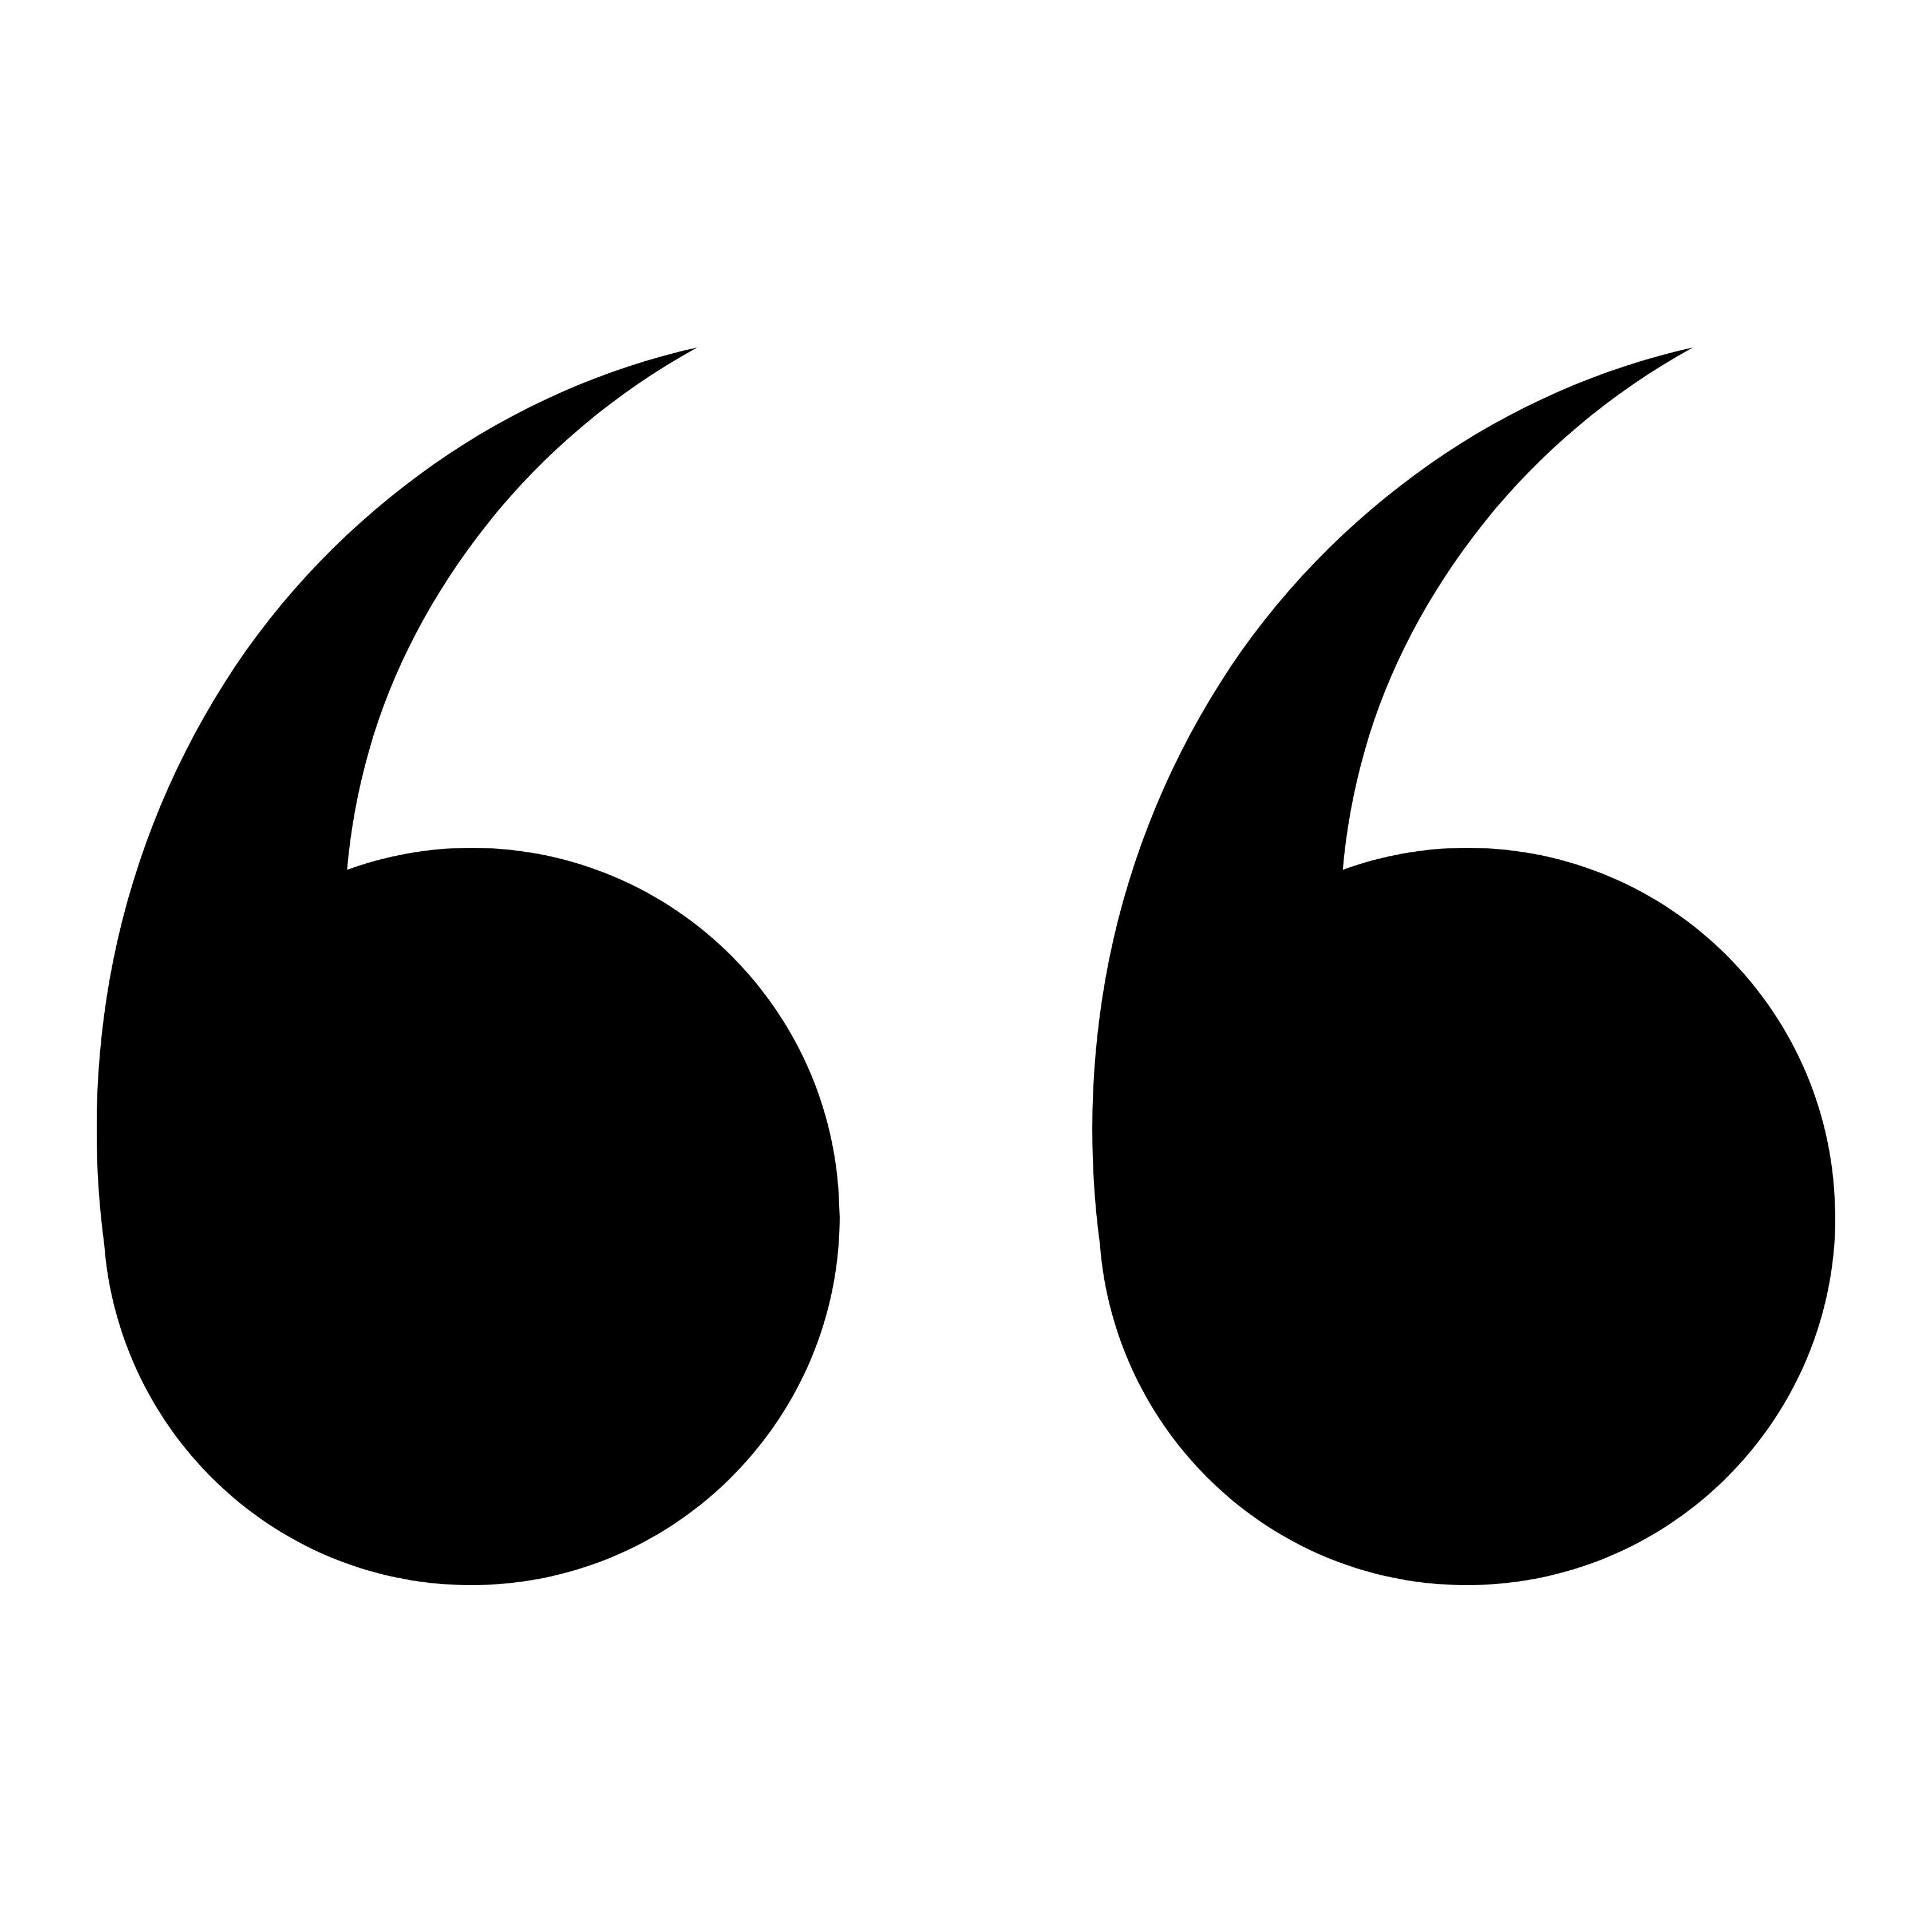
\includegraphics[scale=0.02]{Images/quote2.png}
\hspace{5cm}
    
\dedicationquote{ À mes très chers parents Zahra et Mohammed Said, \\nul mot ne pourra exprimer ma gratitude envers vous.\\ Je n’oublierai jamais vos sacrifices déployés afin de m’élever dignement et d’assurer mon éducation dans les meilleures conditions.\\[0.5cm]
À mes très chères soeurs Hana et Marwa.\\[0.5cm]
À mon très cher frère Hamza.\\[0.5cm]
À toute ma famille.\\[0.5cm]
À toutes mes amies.\\[0.5cm]
Je dédie ce travail…\\
}


\hspace{15cm}
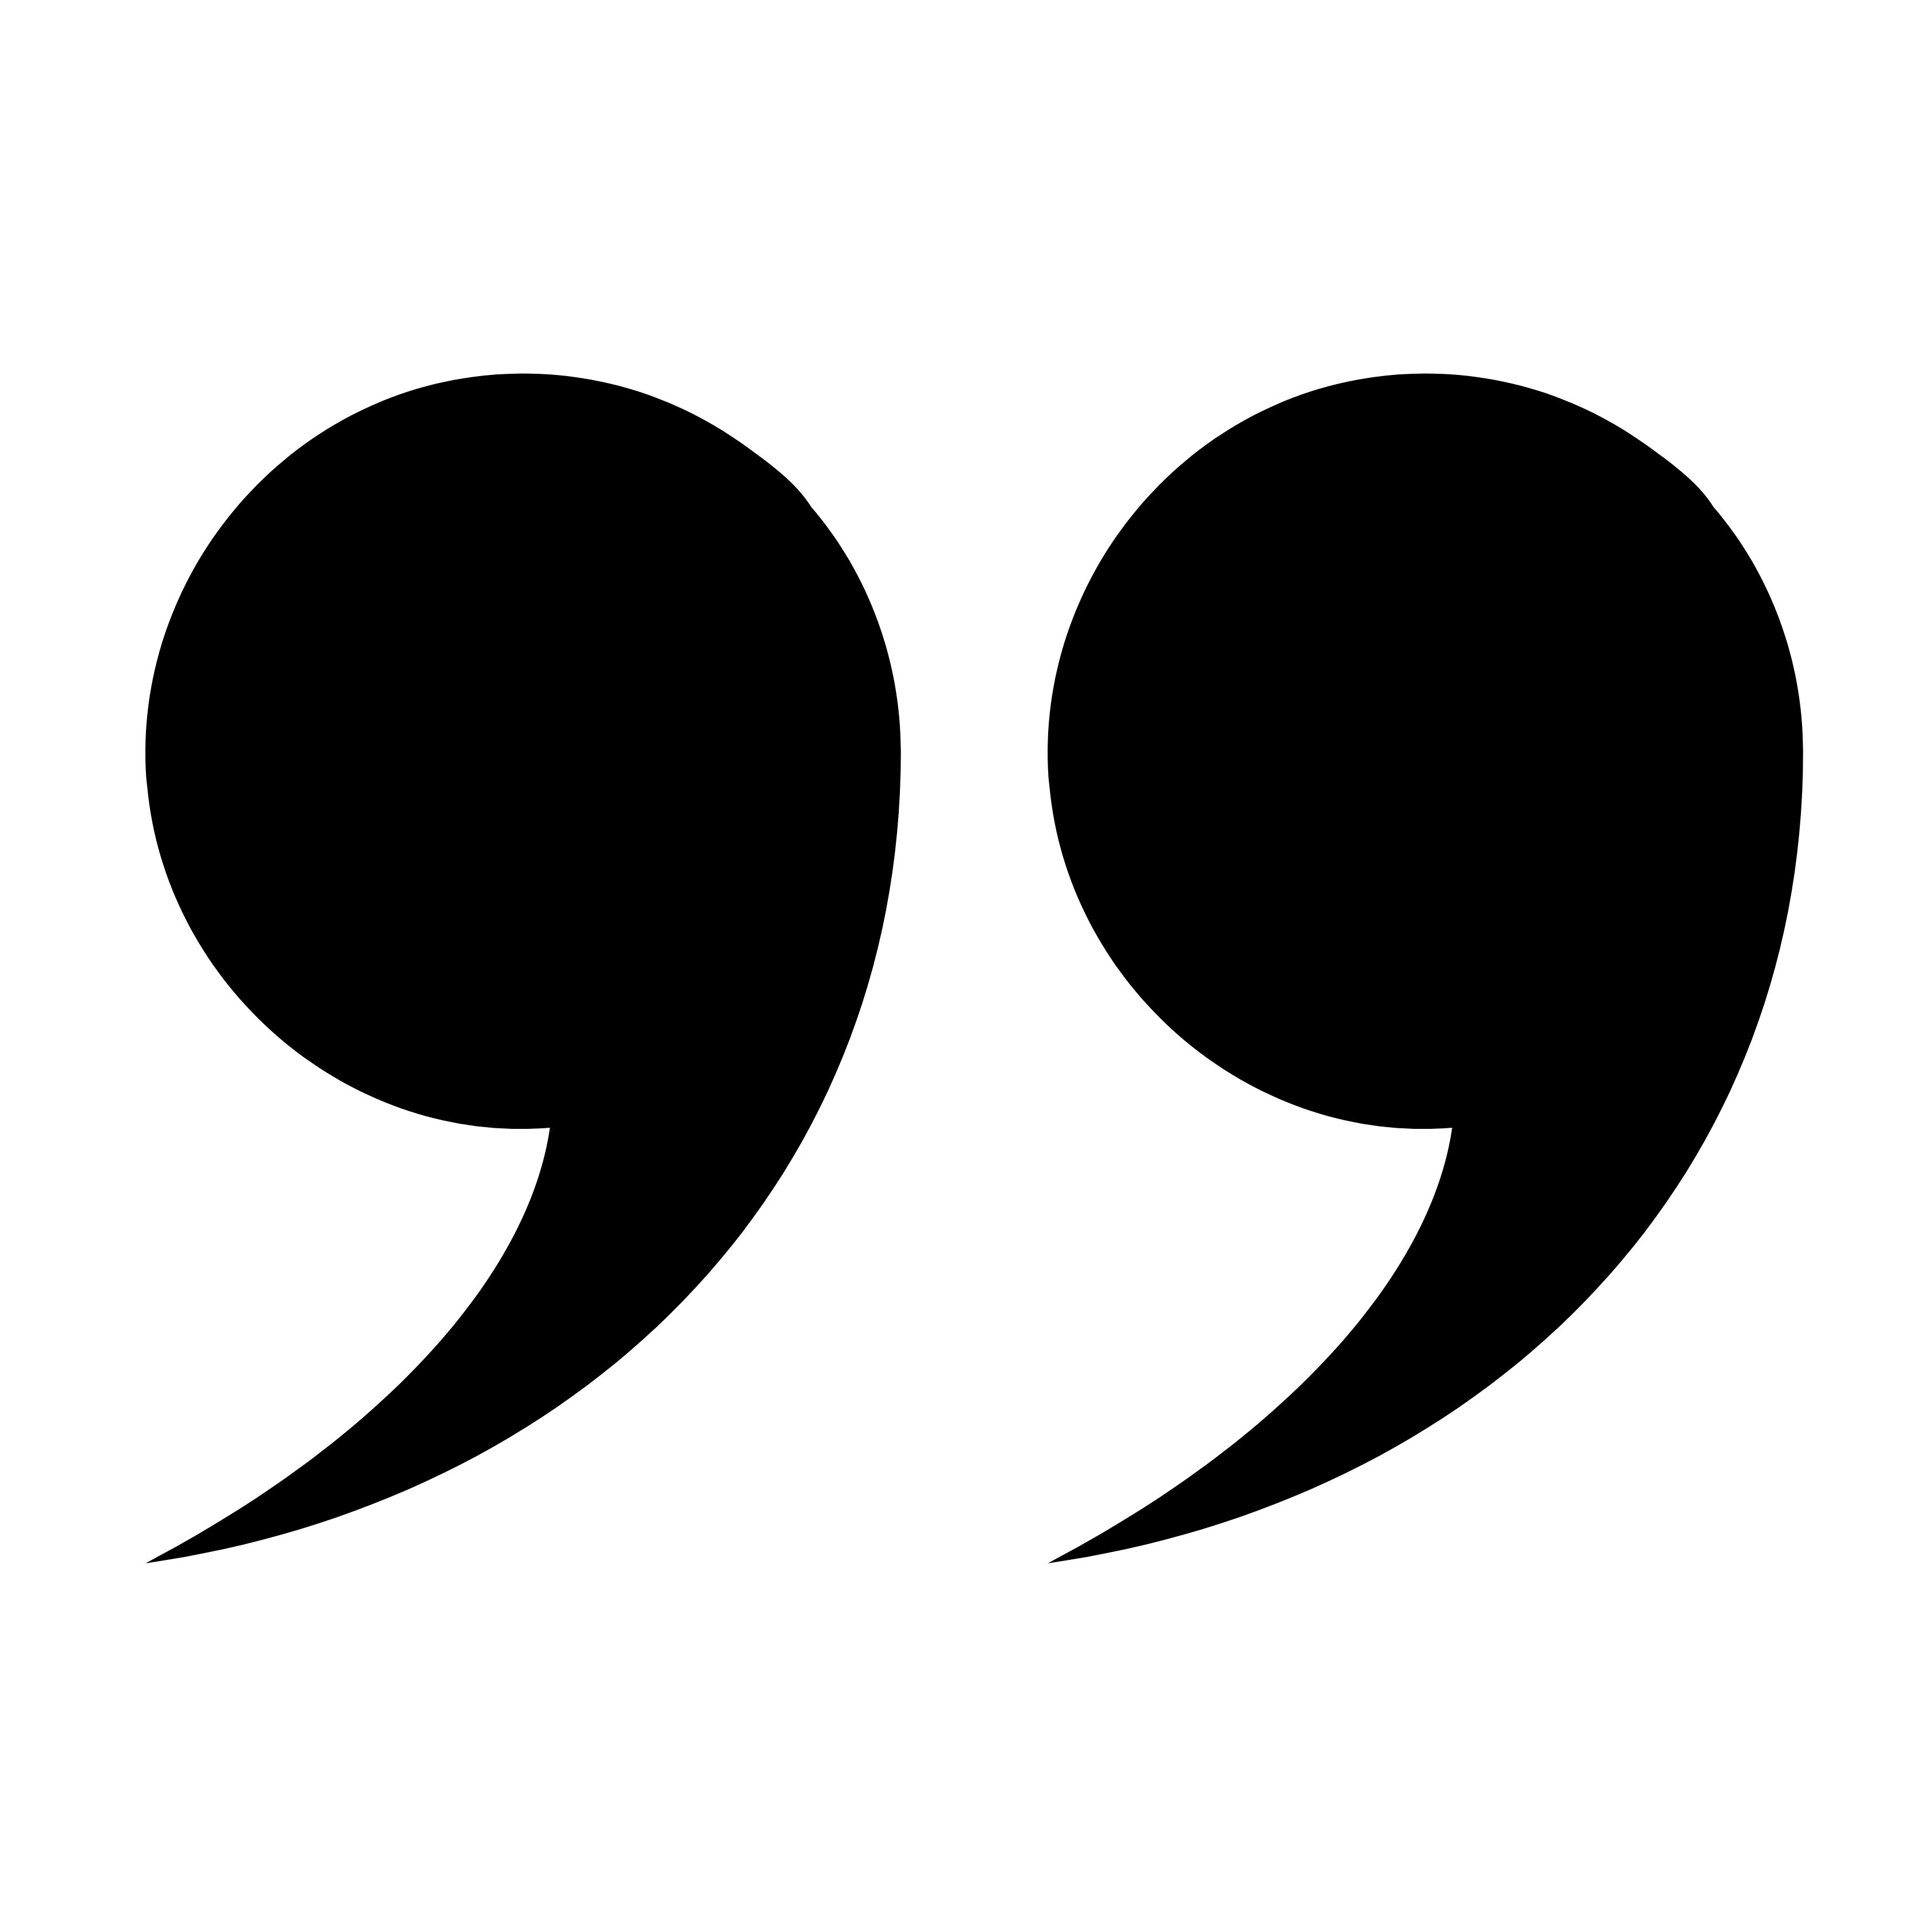
\includegraphics[scale=0.02]{Images/quote1.png}
\vspace{1cm}
\signature{- Soukaina}


%%%% Remerciements %%%%
\large
\chapter*{Remerciements}
\addcontentsline{toc}{chapter}{Remerciements}

\begin{spacing}{1.25}

% \hspace{0.6cm}Je tiens à remercier toutes les personnes qui m'ont soutenu tout au long de la réalisation de ce projet de fin d'études.
% \newline

Tout d’abord, je souhaite remercier mon encadrant interne, \textbf{Pr. HAFIDDI \textsc{Hatim}}, pour ses conseils éclairés et son expertise tout au long de ce projet. Ses propositions constructives ont fortement contribué à la réalisation de ce travail et m’ont permis d’améliorer mes compétences.
\newline

Je tiens à remercier mon encadrant en entreprise 4D, \textbf{M. METWALLI \textsc{Ayoub}}, pour son accompagnement durant le stage et son support en cas de blocage. 
\newline

Je tiens à remercier également les membres de jury \textbf{Pr. BOUSSELAM \textsc{Kaoutar}} et \textbf{Pr. LAGHOUAOUTA \textsc{Youness}} pour l'évaluation du travail réalisé. 
\newline

Mes remerciements s'adressent aussi à l'ensemble du corps enseignant de l'Institut National des Postes et Télécommunications (INPT), pour le temps qu'ils ont consacré pour nous offrir une formation d'excellence et de polyvalence, et à toutes les personnes qui nous ont été d'une aide précieuse. 
\newline

Je tiens à exprimer ma profonde reconnaissance envers ma famille pour leur soutien incessant, leur encouragement constant et leur amour inconditionnel. Leur soutien me pousse toujours à surmonter les défis rencontrés.
\newline

Je tiens à exprimer ma gratitude envers mes amies pour leur soutien et leur support tout au long de ce projet. Leur encouragement et leur présence m'ont été d'une grande aide et ont joué un rôle crucial dans la réussite de ce travail.
\newline

Enfin, je tiens à remercier toutes les personnes qui, de près ou de loin, ont contribué à la réalisation de ce projet. 
\newline
% Leur soutien et leur encouragement ont été précieux et ont rendu cette expérience enrichissante et mémorable.

\end{spacing}

\chapter*{\RL{ملخص}}
% \chapter*{ملخص}

\addcontentsline{toc}{chapter}{Résumé en Arabe}


% \Huge
% \begin{RLtext}
%     \bigskip
%     ملخص
% \end{RLtext}
% 
\includegraphics[scale=22]{Images/ملخص.png} % 
\includepdf[pages=-,fitpaper]{ملخص.pdf}
% 
\includepdf[pages=-]{ملخص.pdf}
\begin{center}
    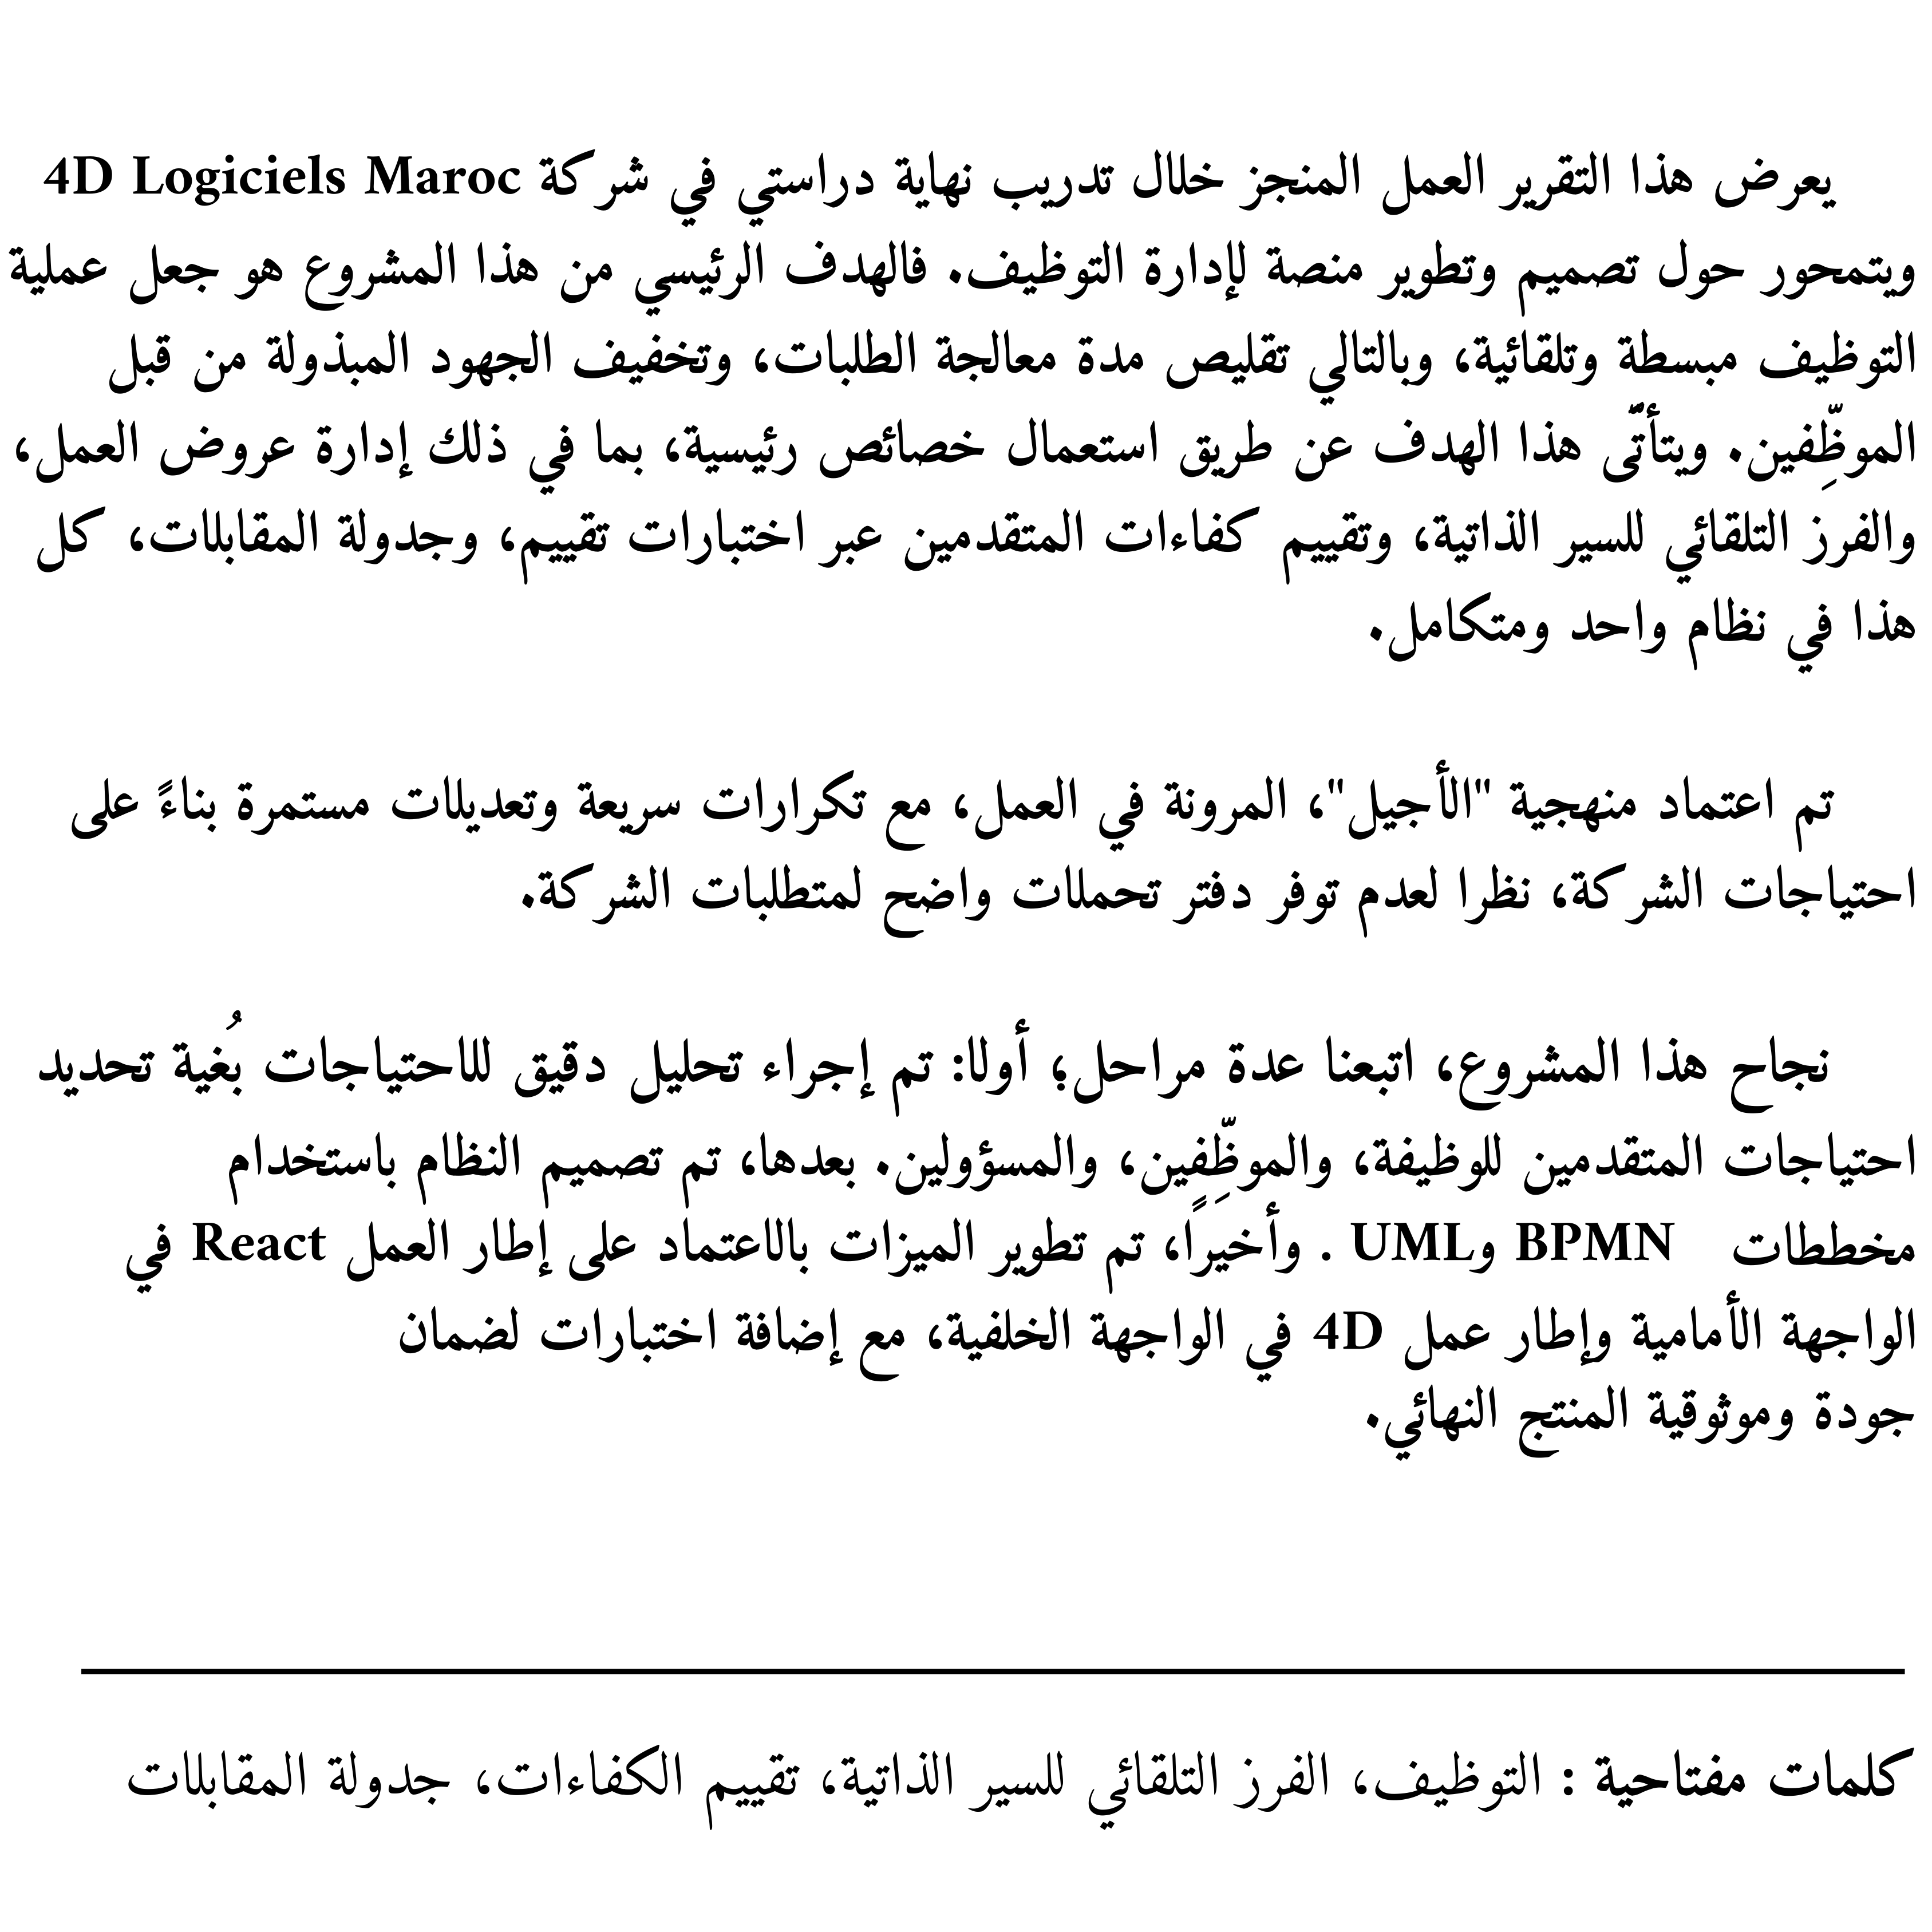
\includegraphics[width=\textwidth]{Images/molkh.png} % 
\includepdf[pages=-,fitpaper]{ملخص.pdf}    
\end{center}
% [width=\textwidth,height=\textheight,keepaspectratio]
% \begin{spacing}{1.25}
    
% \begin{RLtext}
% يقدم هذا التقرير العمل المنجز خلال فترة تدريبي النهائي في شركة 
% 4D Logiciels Maroc،
%  الذي يركز على تصميم وتطوير منصة لإدارة التوظيف. الهدف الرئيسي من هذا المشروع هو تبسيط وأتمتة عملية التوظيف، وبالتالي تقليل أوقات معالجة الطلبات والجهود المبذولة من قبل المجندين. سيتم تحقيق ذلك عن طريق دمج ميزات رئيسية، بما في ذلك إدارة عروض العمل، الفرز التلقائي للسير الذاتية، تقييم كفاءات المتقدمين من خلال اختبارات التقييم، وجدولة المقابلات في نظام متكامل.
% \end{RLtext}
% \vspace{0.7cm}

% \begin{RLtext}
% تم اعتماد منهجية الأجايل، مع تكرارات سريعة وتعديلات مستمرة بناءً على الاحتياجات، نظراً لعدم وجود وثيقة محددة للمتطلبات.
% \end{RLtext}
% \vspace{0.7cm}


% \begin{RLtext}
% لإتمام هذا المشروع، اتبعنا عدة مراحل. أولاً، تم إجراء تحليل دقيق للاحتياجات لتحديد متطلبات المتقدمين، المجندين، والمسؤولين. بعد ذلك، تم تصميم النظام باستخدام مخططات UML وBPMN. وأخيراً، تم تطوير الميزات بناءً على إطار عمل 4D في الجانب الخلفي، مع دمج اختبارات لضمان جودة وموثوقية المنتج النهائي.
% \end{RLtext}

% \end{spacing}
% \vspace{0.7cm}

% \noindent\rule[2pt]{\textwidth}{0.5pt}

% \begin{RLtext} 

% {\textbf{الكلمات المفتاحية}}

% التوظيف، الفرز التلقائي للسير الذاتية، تقييم الكفاءات، جدولة المقابلات
% \\

% \end{RLtext}



% %%%%%%%% Abstract/Résumé %%%%%%%%
\chapter*{Résumé}
\addcontentsline{toc}{chapter}{Résumé}

% \hspace{0.6cm}Le processus de recrutement est un élément crucial pour toute entreprise souhaitant maintenir sa compétitivité sur le marché du travail. Dans le cadre de ce projet de fin d'études réalisé à l'Institut National des Postes et Télécommunications (INPT) en génie logiciel, nous avons entrepris la conception et le développement d'une plateforme de gestion des recrutements pour l'entreprise 4D. Cette plateforme vise à rationaliser et à automatiser les différentes étapes du processus de recrutement, du sourcing des candidats à l'intégration dans l'entreprise.
% \newline

% Le projet s'est articulé autour de plusieurs phases clés, comprenant une analyse approfondie des besoins de l'entreprise, la conception d'une architecture logicielle adaptée, le développement de fonctionnalités sur mesure et la mise en œuvre d'outils de suivi et d'évaluation. En utilisant les meilleures pratiques de développement logiciel et les technologies les plus récentes, nous avons pu créer une plateforme robuste et évolutive, capable de répondre aux exigences spécifiques de l'entreprise 4D.
% \newline

% Les fonctionnalités principales de la plateforme comprennent la gestion des offres d'emploi, la diffusion automatique sur différents canaux de recrutement, la gestion des candidatures, le suivi des entretiens, la collaboration entre les différents intervenants du processus de recrutement et la génération de rapports analytiques pour évaluer l'efficacité des stratégies de recrutement mises en œuvre.
% \newline

% Ce projet a permis de mettre en pratique les connaissances théoriques acquises au cours de notre formation en génie logiciel à l'INPT et de développer des compétences essentielles en matière de conception et de développement de solutions logicielles. Il constitue également une contribution significative à l'optimisation des processus de recrutement de l'entreprise 4D, en permettant une gestion plus efficace et plus transparente des ressources humaines.
% \newline
\begin{spacing}{1.25}

Ce rapport présente le travail effectué lors de mon stage de fin d’études 
chez 4D Logiciels Maroc, axé sur le développement 
d’une plateforme de gestion de recrutement. L'objectif principal 
de ce projet est de simplifier et automatiser le processus de recrutement au sein de l'entreprise 4D,
réduisant ainsi les délais de traitement des candidatures et les efforts effectués par les recruteurs. 
Il y parviendra en intégrant des fonctionnalités principales, notamment la 
gestion des offres d'emploi, le tri automatique des CVs, l'évaluation des compétences des candidats via des tests d'évaluation 
et la planification des entretiens dans un seul système.
\newline

% La méthodologie agile 
% a été adoptée, avec des itérations rapides et des ajustements 
% continus en fonction des besoins, compte tenu de l'absence 
% d'un cahier des charges bien défini. 
% Pour mener à bien ce projet, nous avons suivi plusieurs étapes. 
% Tout d’abord, une analyse de l'existant a été réalisée 
% afin d'identifier les failles du processus actuel, en suite selon chaque module 
% nous avons essaye d'analyser les besoins des utilisateurs et les modeliser via les maquettes, et les différents diagrammes
% UML. En fin le developpement des fonctionnalités de chaque module qui a été entrepris en se 
% basant principalement sur 4D en backend et React en frontend. 
La méthodologie agile a été adoptée, avec des itérations rapides et des ajustements continus en fonction des besoins, 
compte tenu de l'absence d'un cahier des charges bien défini. Pour mener à bien ce projet, nous avons suivi plusieurs étapes. 
Tout d’abord, une analyse de l'existant a été réalisée afin d'identifier les failles du processus actuel. Ensuite, pour chaque module, 
nous avons analysé les besoins des utilisateurs et les avons modélisés via des maquettes et différents diagrammes UML et BPMN. Enfin, le développement 
des fonctionnalités de chaque module a été entrepris en se basant principalement sur 4D pour le backend et React pour le frontend.

% des candidats, 
% des recruteurs et des administrateurs. Ensuite, la modéli-
% sation 
% du système a été effectuée à l’aide des diagrammes UML et BPMN. 
% Enfin, le développement des fonctionnalités a été entrepris en se 
% basant principalement sur 4D en backend et React en frontend, tout en 
% intégrant des tests pour assurer la qualité et la fiabilité du produit final.

\end{spacing}

\vspace{1cm}
\noindent\rule[2pt]{\textwidth}{0.5pt}

{\textbf{Mot clés :} 
recrutement,
tri automatique des CVs,
évaluation des compétences, planification des entretiens
, UML, BPMN, 4D, React}
\\
% \noindent\rule[2pt]{\textwidth}{0.5pt}

% %%%%%%%% Abstract/Résumé %%%%%%%%
    
    \chapter*{Abstract}    
\addcontentsline{toc}{chapter}{Abstract}


\begin{spacing}{1.25}

This report presents the work carried out during my end-of-studies internship at 4D Software Morocco, focused on the design and development of a recruitment management platform. 
The main objective of this project is to simplify and 
automate the recruitment process, thereby reducing processing 
times and efforts by recruiters. This will be achieved by 
integrating principal features, including job offer management, automatic CV sorting, candidate skill evaluation through assessment tests, and interview scheduling into a single coherent system.
\newline

The agile methodology was adopted, involving rapid iterations and continuous adjustments based on needs, due to the absence of a well-defined specifications document. To successfully execute this project, several steps were followed. Initially, an analysis of the existing system was conducted to identify flaws in the current process. Next, user needs for each module were analyzed and modeled using mockups and various UML and BPMN diagrams. Finally, development of each module's functionalities commenced, primarily utilizing 4D for the backend and React for the frontend.
\newline


\end{spacing}

\vspace{1cm}
\noindent\rule[2pt]{\textwidth}{0.5pt}
\textbf{Keywords :} recruitment, automatic CV sorting, competency assessment, interview scheduling, UML, BPMN, 4D, React
%%%%%%%%%%%%%%%%%%%%%%%%%%%%%%%%%%%%%%%%%%%%%%%%%%%%%%%
% \pagestyle{empty}\strut \null


% %%%%%%%%%% ملخص %%%%%%%%%%

% %%%%%%%% Acronyms %%%%%%%%

%%%% List of Figures %%%%%
\listoffigures
\addcontentsline{toc}{chapter}{Liste des figures}

% \pagestyle{empty}
% \newpage
% \strut \null
% \newpage

\listoftables
\addcontentsline{toc}{chapter}{Liste des tableaux} 

\chapter*{Liste des abréviations}

\begin{spacing}{1.5}
    
\begin{tabular}{l  l}    
    % \textbf{AES} &  Advanced Encryption Standard  \\
    \textbf{BPMN} & Business Process Modeling Notation \\
    \textbf{CSS} & Cascading Style Sheets \\
    \textbf{CV} & Curriculum Vitae \\
    \textbf{E2E} & End to End \\
    \textbf{HTML} & Hypertext Markup Language \\ 
    % \textbf{JSON} & JavaScript Object Notation \\
    \textbf{ORDA} & Object Relational Data Access \\
    % \textbf{PAO} & Publication Assistée par Ordinateur \\
    % \textbf{PDF} & Portable Document Format \\
    \textbf{REST} & Representational State Transfer \\
    % \textbf{SOA} & Service-Oriented Architecture \\
    % \textbf{SVN} & Subversion \\
    \textbf{UML} & Unified Modeling Language \\
    
\end{tabular}
\end{spacing}


%tables are added automatically here

%%%%%%%% Contents %%%%%%%%
\tableofcontents
\addcontentsline{toc}{chapter}{Table des matières}
\chapter*{Introduction}
\addcontentsline{toc}{chapter}{Introdcution}
% Dans un monde où la compétitivité économique et la recherche des nouveaux talents
% sont en pleine croissance ; présentant, de ce fait, un enjeu et une priorité majeurs pour la
% majorité des entreprises. Cette capacité à cibler, attirer et recruter les meilleurs profils qui
% s’alignent avec les besoins internes est désormais une priorité stratégique pour assurer le
% développement à long terme des organisations. Néanmoins, les méthodes traditionnelles de
% recrutement se heurtent à une myriade de défis. En effet, ces dernières nécessitent souvent
% des efforts immenses de la part des recruteurs pour examiner manuellement un grand
% nombre de candidatures, ce qui les rend alors sujettes à des erreurs humaines, des retards
% ou à des inexactitudes dans l’évaluation des profils. En outre, la lenteur des échanges entre
% les différentes parties prenantes et les problèmes de communication ajoutent des obstacles
% supplémentaires à un processus déjà complexe.
% \newline

% Face à ces défis, la digitalisation du processus de recrutement émerge comme une
% solution prometteuse, offrant d’une part aux candidats la possibilité de consulter toutes les
% offres disponibles, postuler pour celles-ci et suivre l’état d’avancement de sa candidature.
% D’une autre part, cette solution permet aux recruteurs d’utiliser des outils d’analyse des
% données pour évaluer les candidatures, faciliter la communication entre toutes les parties
% prenantes, et d’optimiser les ressources humaines et financières en réduisant les coûts
% liés à la gestion des candidatures et en accélérant les délais de recrutement. C’est dans
% ce contexte ou s’inscrit mon projet de fin d’études ayant pour objectif primordial de
% concevoir et de développer une plateforme dédiée à la digitalisation et la centralisation
% du processus de recrutement au sein de 4D Logiciels qui répondra bien évidemment à ces
% problématiques en améliorant l’efficacité du processus actuel de recrutement.  
% \newline

% Afin de présenter le travail réalisé, ce rapport est structuré en quatre parties principales. 
% Le premier chapitre met en lumière l’organisme d’accueil de mon stage : 4D Logiciels Maroc,
%  le contexte général du projet ainsi que la démarche suivie pour le développement
% du projet. Le deuxième chapitre donne une vision globale sur l’existant et la spécification
% des besoins. Le troisième chapitre est consacré à la modélisation UML et BPMN de la
% solution, ainsi, il met en évidence les outils technologiques utilisés. Finalement, le dernier
% chapitre présente la réalisation du projet en mettant en exergue l’architecture technique
% adoptée et les différentes interfaces réalisées.



Le recrutement est crucial pour toute entreprise, influant directement sur sa performance et sa réussite dans un marché du travail compétitif en constante évolution. Ce rapport se concentre sur la digitalisation des processus de recrutement chez 4D Logiciels Maroc, dans le cadre de mon stage de fin d'études à l'INPT. Le projet vise à développer une plateforme innovante pour simplifier et automatiser les différentes étapes du recrutement, répondant ainsi aux besoins contemporains du marché du travail.
\newline

Ce projet s'articule autour de plusieurs axes majeurs. Tout d'abord, il cherche à centraliser et optimiser les processus de recrutement en intégrant des fonctionnalités avancées telles que la gestion des offres d'emploi, le tri automatique des CVs et la planification des entretiens. Ensuite, il s'appuie sur les meilleures pratiques en ingénierie logicielle pour garantir la solidité et l'efficacité de la solution. Enfin, il adopte une démarche agile, favorisant des itérations rapides et une adaptation continue pour répondre aux besoins changeants de l'entreprise et du marché.
\newline

Le projet sera structuré en plusieurs chapitres. Nous commencerons par présenter le contexte général du projet, suivi par une analyse et une spécification des besoins de l'entreprise en matière de recrutement. Ensuite, nous détaillerons la conception de la solution, en mettant en avant les différentes fonctionnalités prévues. Enfin, nous aborderons l'implémentation de la solution et sa validation pour assurer sa conformité aux attentes et son bon fonctionnement.
\newline

% Define the page style
\fancypagestyle{chapterstyle}{
   \fancyhead[L]{\nouppercase{\rightmark}}
   \fancyhead[R]{Projet de fin d'etudes 2023-2024}
   \fancyfoot[C]{\vspace{20pt}\thepage} % Adjust the vertical space here
   \setlength{\headheight}{20pt}
   \setlength{\footskip}{30pt} % Adjust the value as needed
}

\chapter{Contexte Général}
\pagestyle{chapterstyle}
Ce premier chapitre a pour objectif de présenter
l’organisme d’accueil, son historique, ses objectifs
et ses activités. Il fournira également une 
description du contexte du projet, en mettant
en évidence le problème qu’il vise à résoudre, 
les attentes associées, ainsi que la gestion et 
la planification de sa mise en œuvre.



\newpage
\vspace{1cm}
\section{Introduction}
% \vspace{1cm}

% Dans ce chapitre nous allons commencer par une présentation de l’organisme d’accueil, 
% son histoire, ses services et bien d’autres informations, 
% puis nous aborderons la méthodologie de travail pendant 
% les quatre mois de stage et finalement la manière dont nous avons géré notre projet.

Le premier chapitre vise à introduire le projet de manière générale. 
Il est divisé en trois parties principales, chacune ayant 
plusieurs sections. La première partie offre une courte présentation 
de 4D Logiciels Maroc, en expliquant son architecture, ses missions 
ainsi que le groupe 4D et ses produits. La deuxième partie situe 
le projet dans son contexte en décrivant son cadre général, 
la problématique à la base de sa création et les différents 
objectifs visés. Enfin, la dernière partie détaille la méthode 
de conduite de projet choisie.


%%%%%%%%%%%%%%%%%%%% SECTION 2 %%%%%%%%%%%%%%%%%%%%%%%

\section{Présentation de l’organisme d’accueil}

Fondée en 1984 par Laurent Ribardière, 4D logiciel est une entreprise de conseil et de
développement de logiciels dans le domaine des systèmes d’informations, de l’organisation
et de l’informatique dont le siège social se situe à Clichy (Île-de-France).
\newline

Laurent Ribardière a créé 4D avec une seule ambition : simplifier la création des
applications professionnelles pour les entreprises grâce à une base de données relationnelles
entièrement graphique.
\newline

4D est devenue ainsi l’un des premiers éditeurs de logiciels français avec un rayonnement international grâce à sa présence sur les cinq continents et des filiales dans plus de
dix pays dont le Maroc (4D Logiciels Maroc).
\newline

Le succès de 4D vient de sa capacité à répondre aux enjeux de son époque, grâce à
une plateforme évolutive, simplifiant la création d’expériences clients réussies sur mobile,
web, desktop.


\begin{figure}[h]
    \centering
    
\includegraphics[scale=1.5]{Images/logo-4d.jpg} % Replace with the actual filename of the IBM logo image
    \caption{Logo 4D}
    \label{fig:Logo4D}
\end{figure}



%%%%%%%%%%%%%%%%%%%% subsection 1 %%%%%%%%%%%%%%%%%%%%%%%

\subsection{Histoire de 4D}

L’entreprise 4D Logiciels, une entreprise faisant partie du marché de l’édition logicielle
dont le siège est situé en France.
\newline
\newline
\newline
\newline


\begin{figure}[h]
    \centering
    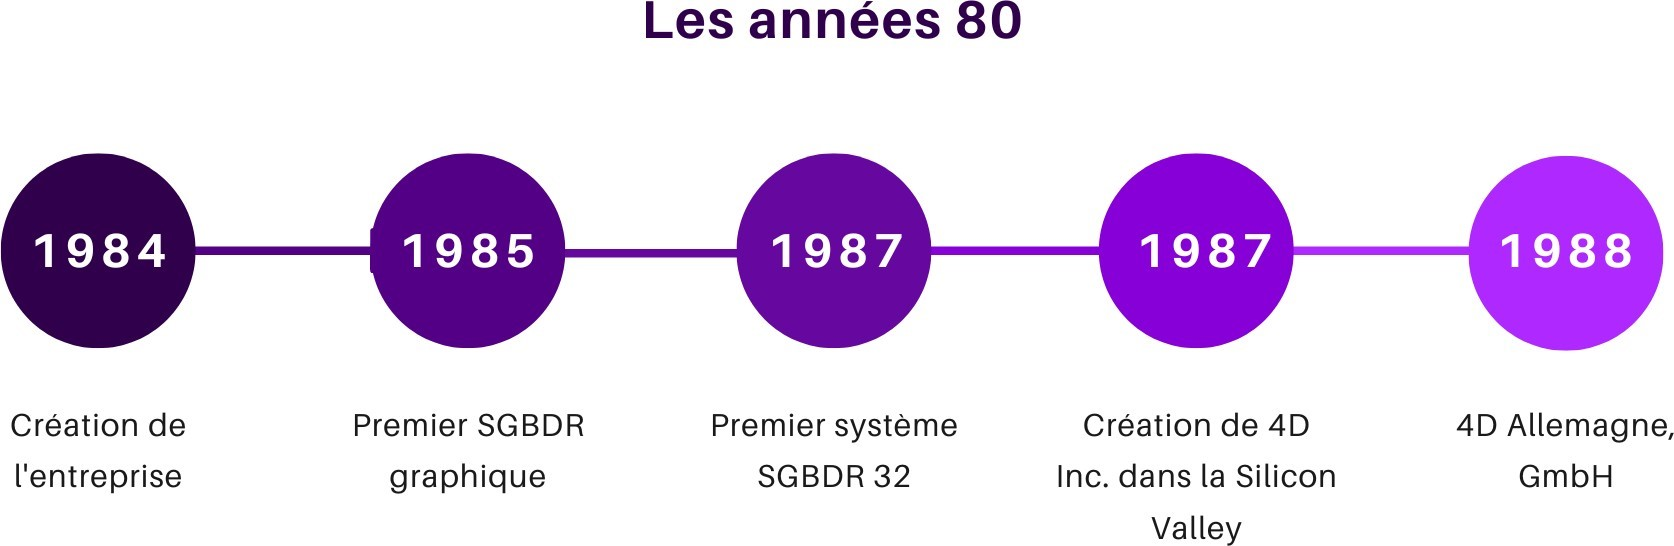
\includegraphics[scale=0.3]{Images/80.jpg} % Replace with the actual filename of the IBM logo image
    \caption{Les années 80}
    \label{fig:Histoire80}
\end{figure}


Crée en 1984, 4D Logiciels est reconnu par ses outils de développement innovants permettant de créer des solutions professionnelles performantes et fiables au service des entreprises.
En 1987, 4D Logiciels propose le premier système de gestion de base de données relationnel fonctionnant sur un système 32-bits, puis conserve sa place de leader en offrant le premier :
\begin{itemize}
    \item • Client-serveur intégré.
    \item • Serveur web intégré.
    \item • Système de partage d’applications dynamique intégré.
\end{itemize}
\vspace{1cm}

\begin{figure}[h]
    \centering
    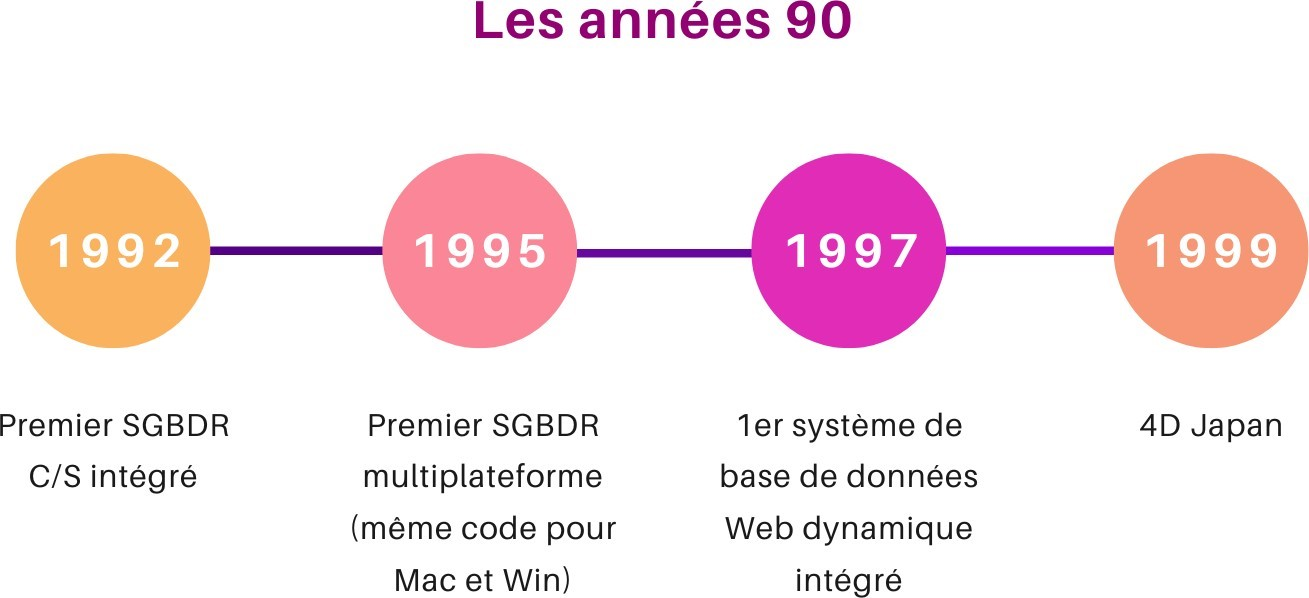
\includegraphics[scale=0.3]{Images/90.jpg} % Replace with the actual filename of the IBM logo image
    \caption{Les années 90}
    \label{fig:Histoire90}
\end{figure}
% \vspace{lcm}

En 1997, 4D décide de s’investir dans le Web en donnant lieu 
à un serveur Web dynamique. Ce qui aide les développeurs à servir
à la fois des applications client-serveur et des applications
Web sans modifier le code. 4D conserve par la suite ce produit 
en lançant à chaque fois des nouvelles versions.
\vspace{6cm}

\begin{figure}[h]
    \centering
    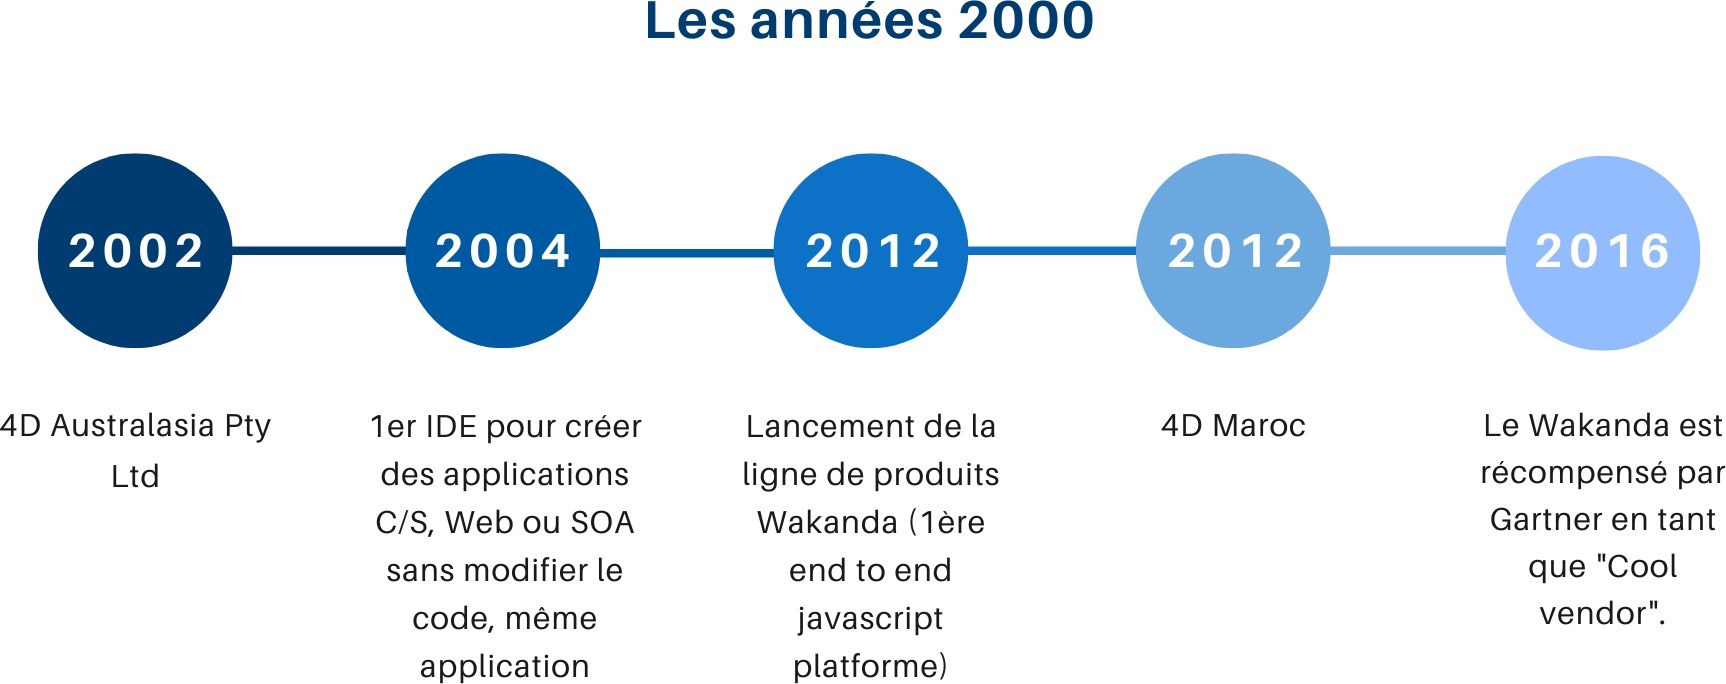
\includegraphics[scale=0.3]{Images/20.jpg} % Replace with the actual filename of the IBM logo image
    \caption{Les années 2000}
    \label{fig:Histoire90}
\end{figure}

La version 4D 2004 se lance en tant qu’un produit permettant aux développeurs 
de créer à la fois des applications autonomes, client-serveur, Web, 
ainsi que des applications orientées Services (SOA) sans rajouter 
aucun changement au niveau du code.
Plus récemment, 4D dispose d’une plateforme de développement 
en JavaScript qui facilite la création des applications 
professionnelles en utilisant la gamme de produits Wakanda.


%%%%%%%%%%%%%%%%%%%% subsection 2 %%%%%%%%%%%%%%%%%%%%%%%

\subsection{Le Langage 4D}

4D est une plateforme de développement productive qui permet aux clients
 de se concentrer sur leur modèle de données et les règles 
 et spécificités de leur métier [1].
 Le langage 4D prend en charge l’exécution native 
 de leur code applicatif sous macOS et Windows. 
 4D Serveur exécute leurs applications simultanément sur les postes de travail
/ clients mobiles et sur le Web. Ils peuvent déployer des applications 
entièrement personnalisées sous leur propre marque.
 4D est un système de gestion de base de données 
 relationnelle disposant d’un langage de programmation 
 de la quatrième génération.
\newline

Environnement de développement intégré, 4D intègre :
\begin{itemize}
    \item un compilateur
    \item un débogueur
    \item un système de sauvegarde et de réplication
    \item un serveur Web
    \item un serveur et client de services web
\end{itemize}

\begin{figure}[h]
    \centering
    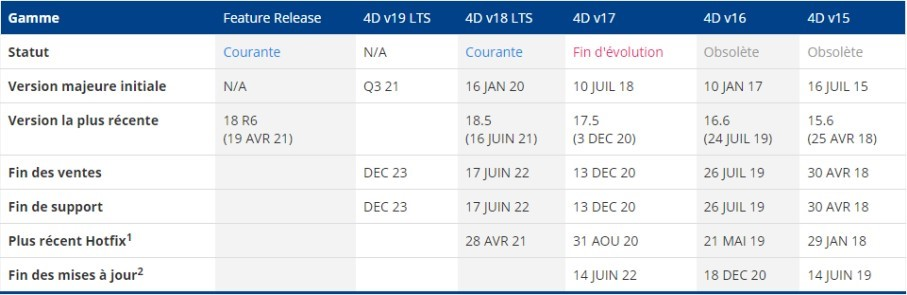
\includegraphics[scale=0.7]{Images/versions.jpg} % Replace with the actual filename of the IBM logo image
    \caption{Anciennes versions de 4D}
    \label{fig:AncienneVersions}
\end{figure}

\vspace{6cm}
4D v18 marque un véritable tournant dans l’histoire de 4D. Cette version propose non seulement de
multiples nouvelles fonctionnalités, mais aussi l’amélioration de fonctions existantes. Elle introduit la gestion de version pour changer 
la façon dont les équipes collaborent. Le format texte des bases projets permet désormais de tirer pleinement parti des systèmes de gestion de version
(par exemple, Git, SVN, etc.). Autre fonctionnalité qui fait ses débuts dans cette nouvelle version : une solution intégrée de chiffrement des données, 
offrant en un seul clic une sécurité maximum aux données des clients. Ces outils de chiffrement sont basés sur l’un des algorithmes les plus sûrs : 
Advanced Encryption Standard (AES). ORDA (Object Relational Data Access), la technologie révolutionnaire d’accès et de présentation 
des données, apporte également son lot de nouvelles fonction- nalités, telles que le Datastore distant, ouvrant de nouvelles perspectives et optimisant les 
performances du client/serveur. Les applications métiers peuvent facilement être dé- ployées sur des appareils mobiles avec 4D for iOS, une solution 
entièrement intégrée à 4D. De plus, 4D Write Pro, outil de PAO intégré à 4D, poursuit sa montée en puissance, le langage de programmation 4D s’enrichit et apporte de nouvelles commandes destinées à améliorer l’expérience de développement.
\newline

La dernière version du produit 4D, 4D v19 R8, est une version encore plus améliorée qui offre de nouvelles 
fonctionnalités. Cette version est particulièrement intéressante pour les développeurs et les utilisateurs de 4D,
car elle leur permet de bénéficier de performances accrues et d’une expérience utilisateur améliorée.
En effet, les améliorations apportées à cette version ont été conçues pour répondre aux besoins des utilisateurs de manière plus efficace.
\newline

La version 4D v20 est actuellement en version beta, ce qui signifie 
qu’elle est encore en phase de test. Cette version n’est pas encore 
disponible pour une utilisation générale, mais elle est plutôt réservée 
à un groupe restreint de testeurs qui vont l’évaluer et signaler 
les éventuels problèmes ou bugs. Cette phase de test permet à l’équipe 
de développement de recueillir des commentaires et des suggestions de la part 
des testeurs afin d’améliorer la qualité du logiciel avant sa sortie officielle. 
En bref, la version 4D v20 est en mode testing pour s’assurer qu’elle est stable et 
fiable avant d’être rendue disponible pour le grand public.

\vspace{0.5cm}

\begin{figure}[h]
    \centering
    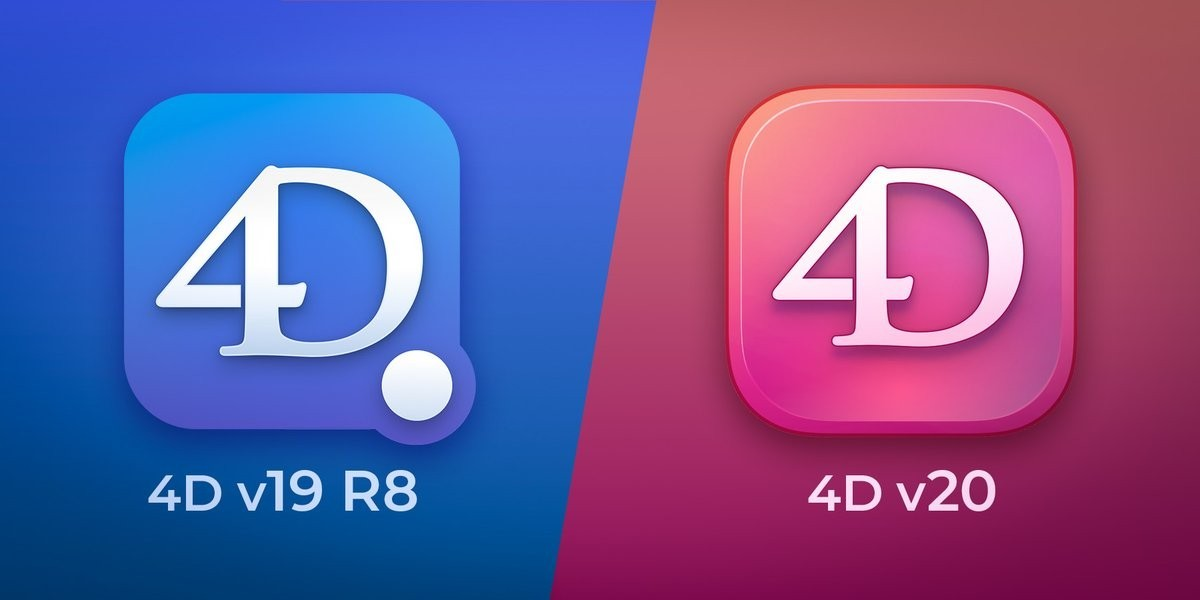
\includegraphics[scale=0.3]{Images/v19v20.jpg} % Replace with the actual filename of the IBM logo image
    \caption{les deux nouvelles versions de 4D}
    \label{fig:v19v20}
\end{figure}


%%%%%%%%%%%%%%%%%%%% subsection 3 %%%%%%%%%%%%%%%%%%%%%%%

\subsection{La structure du groupe 4D}
Acteur dans le métier de l’édition de logiciel, la société
4D développe et commercialise depuis plus de trente 
ans à travers le monde, une plateforme logicielle 
intégrée qui accélère et simplifie le développement
et le déploiement des applications métiers des clients finaux.
Le groupe 4D est composé d’un siège social situé en France, 
et de cinq filiales situées aux États-Unis, en Allemagne, 
en Australie, au Japon, et au Marocj[1]. À l’écoute permanente 
de leurs besoins et des évolutions technologiques, 
la société propose une aven- ture passionnante dans un 
contexte multiculturel à travers ses différentes implantations 
à l’international (Sydney, Tokyo, San José, Munich, Rabat).

\vspace{1cm}

\begin{figure}[h]
    \centering
    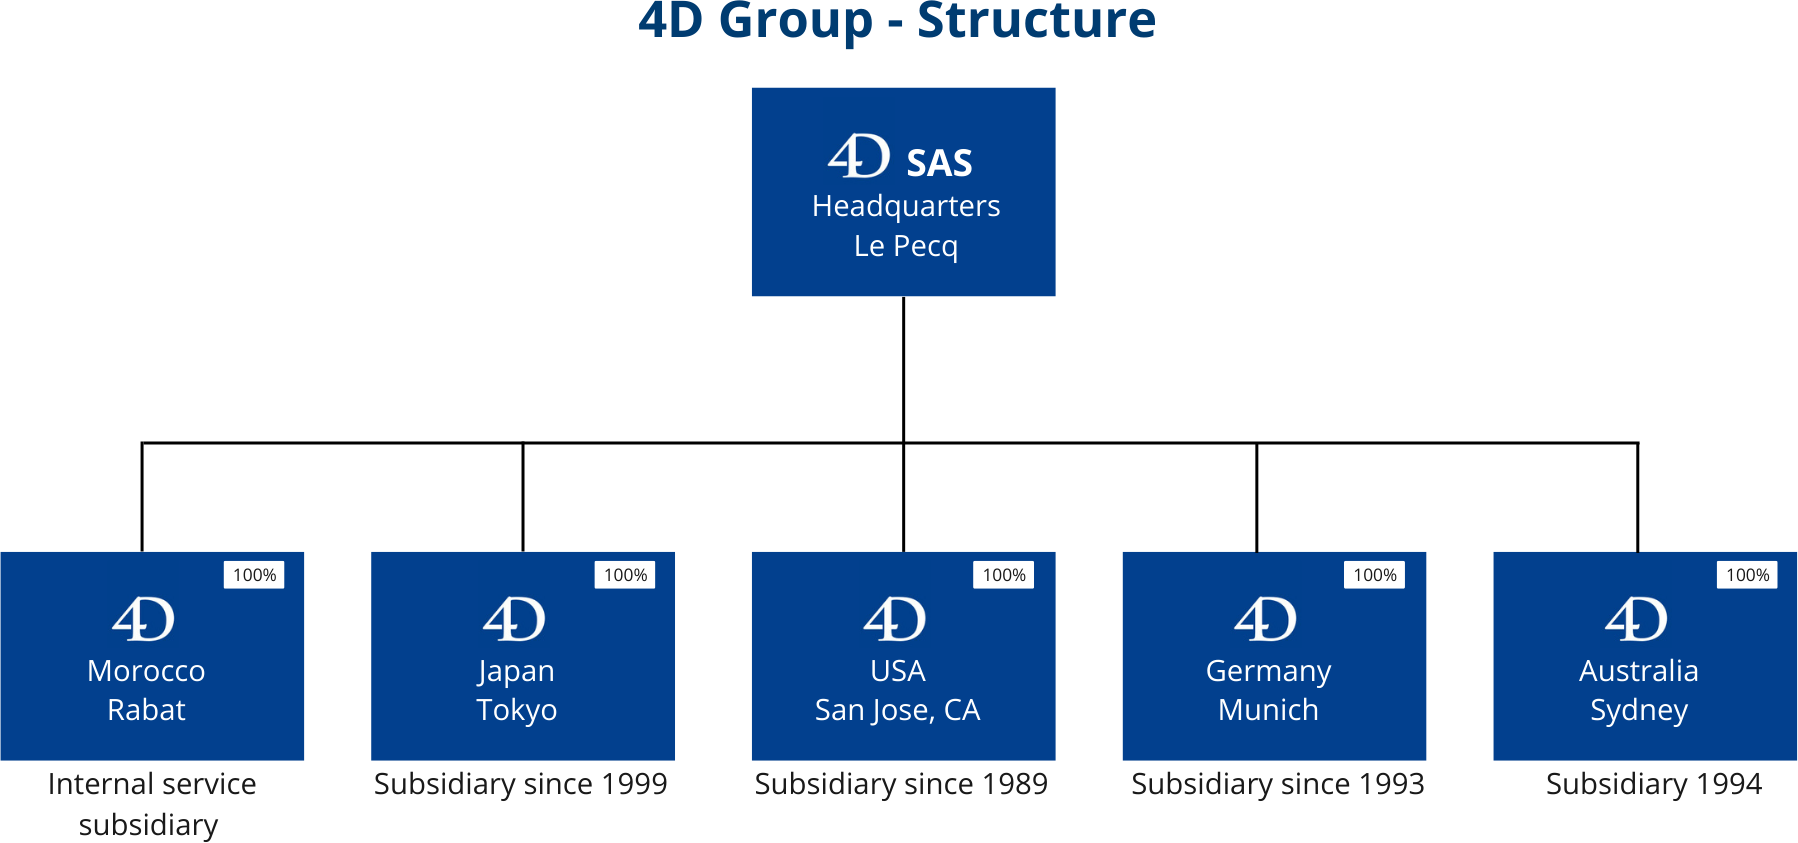
\includegraphics[scale=0.35]{Images/groupe.png} % Replace with the actual filename of the IBM logo image
    \caption{Le groupe 4D dans le monde}
    \label{fig:groupe}
\end{figure}

Comme toute société renommée, 4D recourt à ses différents partenaires 
pour un rendu meilleur et un niveau d’expertise plus crédible. 4D connaît aussi 
une présence internatio- nale grâce à ses partenaires et ses distributeurs éparpillés 
dans le monde, comme montre la figure suivante :

\begin{figure}[h]
    \centering
    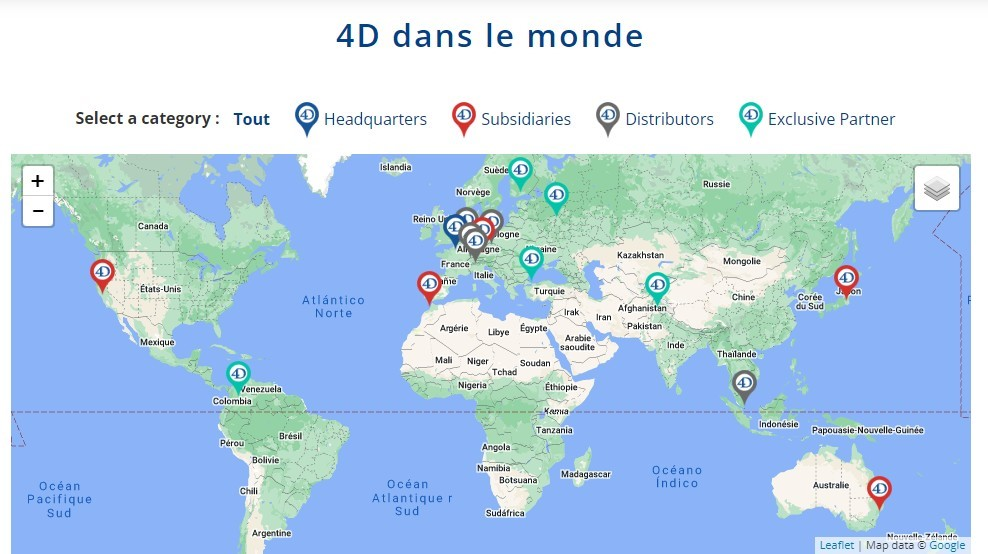
\includegraphics[scale=0.6]{Images/carte.jpg} % Replace with the actual filename of the IBM logo image
    \caption{Les points de présence des partenaires et des distributeurs de 4D}
    \label{fig:carte}
\end{figure}

La figure ci-dessous montre la direction générale de l’entreprise 4D logiciels :

\begin{figure}[h]
    \centering
    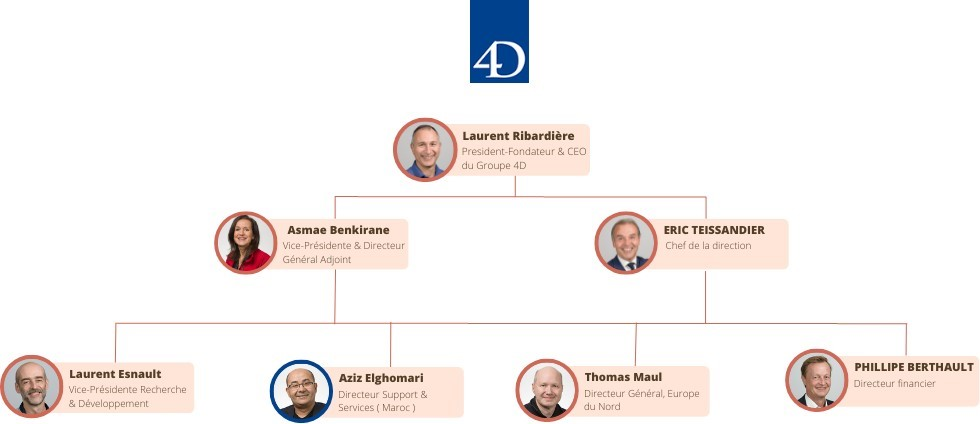
\includegraphics[scale=0.6]{Images/direction.jpg} % Replace with the actual filename of the IBM logo image
    \caption{La Direction Générale de 4D}
    \label{fig:direction}
\end{figure}

%%%%%%%%%%%%%%%%%%%% subsection 4 %%%%%%%%%%%%%%%%%%%%%%%
\subsection{Les domaines Métiers et les clients 4D}
4D intervient dans une diversité de domaines, comme 
la santé, l’éducation, l’adminis- tration, la gouvernance, 
et les télécommunications. La figure 1.6 montre le pourcentage 
qu’occupe chaque domaine dans son activité.

\begin{figure}[h]
    \centering
    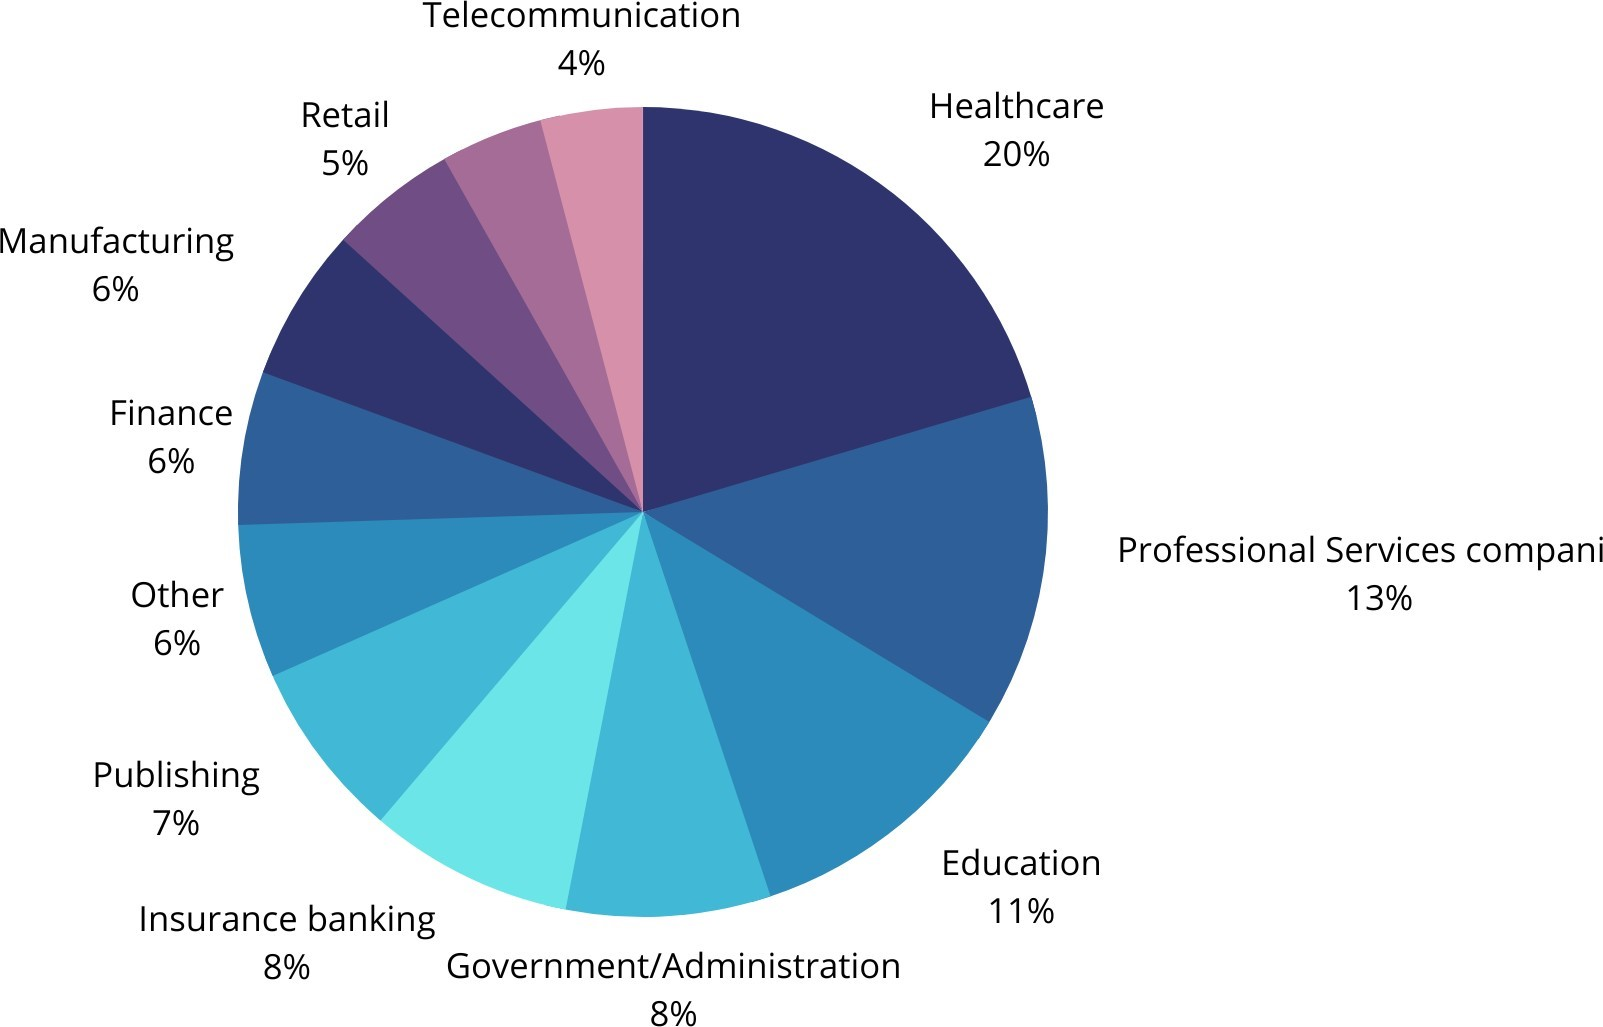
\includegraphics[scale=0.3]{Images/domaineMetier.jpg} % Replace with the actual filename of the IBM logo image
    \caption{Les domaines métiers de 4D en pourcentage}
    \label{fig:domaineMetier}
\end{figure}


%%%%%%%%%%%%%%%%%%%% SECTION 3 %%%%%%%%%%%%%%%%%%%%%%%

\section{Présentation du projet}
\subsection{Cadre du projet}
Dans un environnement où la concurrence pour attirer les meilleurs talents
 est de plus en plus intense, les entreprises doivent disposer d'outils 
 efficaces pour gérer leur processus de recrutement. Actuellement, 
 4D Logiciels utilise un système disparate et manuel pour le recrutement, 
 ce qui entraîne des inefficacités et des pertes de temps. Cette situation 
 rend difficile la gestion des candidatures, la traçabilité des étapes de 
 recrutement, et la communication entre les recruteurs et les candidats.

Afin de renforcer le niveau de ses collaborateurs, 4D Logiciels souhaite 
simplifier et moderniser son processus de recrutement. L'objectif est de passer 
d'un système essentiellement manuel à une solution plus intégrée et automatisée, 
permettant d'améliorer l'efficacité, de réduire les délais de recrutement, 
et d'offrir une meilleure expérience aux candidats.

\subsection{Problématique}
L'entreprise 4D Logiciels est confrontée à une gestion inefficace
 de ses processus de recrutement, notamment lorsqu'elle publie 
 des offres d'emploi et ouvre des opportunités de stage annuelles.
4D Logiciels reçoit un grand nombre de candidatures non triées,
provenant de divers domaines, ce qui rend difficile la
sélection des candidats les plus appropriés. Les méthodes 
traditionnelles utilisées, telles que les emails, les tableurs 
et les calendriers, ne permettent pas de gérer efficacement 
ce flux de candidatures. De plus, les applications de recrutement
 disponibles sur le marché ne répondent pas pleinement aux 
 besoins spécifiques de l'entreprise en termes de processus 
 de recrutement.

En considérant les défis actuels du processus de recrutement chez
 4D Logiciels, une interrogation primordiale se profile : 
 comment transformer efficacement le processus de recrutement 
 afin de surmonter les obstacles liés au traitement manuel des 
 candidatures, à la dispersion des données et à la gestion 
 disjointe des entretiens, assurant ainsi une sélection de 
 candidats plus optimale et équitable pour l'organisation ?


\subsection{Les objectifs}

Pour répondre efficacement à la problématique identifiée,
la solution proposée doit satisfaire les objectifs suivants :

\begin{itemize}
    \item Centraliser et Automatiser la Gestion des Candidatures
    \item Améliorer la Sélection des Candidats 
    \item Optimiser la Traçabilité et la Suivi des Étapes de Recrutement 
    \item Faciliter la Communication et la Collaboration 
    \item Analyser et Optimiser les Performances du Processus de Recrutement 
    \item Offrir une Meilleure Expérience Candidat 
\end{itemize}

%%%%%%%%%%%%%%%%%%%% SECTION 4 %%%%%%%%%%%%%%%%%%%%%%%
\section{Déroulement du projet}





% Define the page style
\fancypagestyle{chapterstyle}{
   \fancyhead[L]{\nouppercase{\rightmark}}
   \fancyhead[R]{Projet de fin d'études 2023-2024}
   \fancyfoot[C]{\vspace{20pt}\thepage} % Adjust the vertical space here
   \setlength{\headheight}{20pt}
   \setlength{\footskip}{30pt} % Adjust the value as needed
}


\chapter{Analyse et spécification des besoins}
\pagestyle{chapterstyle}

\newpage
\vspace{1cm}

%-------------Spécifications des exigences-----------

\section{Introduction}
Dans ce chapitre, nous menons une étude approfondie du processus existant en mettant
en évidence les solutions de gestion de recrutement actuellement adoptées par 4D, ainsi
que les plateformes et les outils qui existent déjà sur le marché. Cela est dans l’objectif
de cerner les besoins fonctionnels et non fonctionnels auxquels doit répondre le projet.

\section{Analyse de l'existant}
Actuellement, chez 4D, il n’existe pas de plateforme centralisée pour gérer le processus
de recrutement. Les recruteurs utilisent plusieurs outils qui varient selon les différentes
étapes du processus, incluant LinkedIn, Gmail entre autres. Cette diversification des outils
entraîne plusieurs problèmes tels que le risque de perte d’informations, des difficultés de
coordination, ainsi qu’un temps de traitement des candidatures plus élevé. Ce processus
passe en fait par plusieurs étapes, notamment :

\begin{enumerate}
   \item \textbf{Publication des annonces :} le processus de recrutement débute par la publication des offres d’emploi sur LinkedIn. Les recruteurs de 4D rédigent des annonces
   détaillées incluant les qualifications requises, les responsabilités du poste, ainsi que
   les informations sur l’entreprise. Ces annonces contiennent une adresse e-mail dédiée
   où les candidats peuvent envoyer leurs candidatures..
   \item \textbf{Réception des candidatures :} Les candidats intéressés par les postes publiés
   envoient leur dossier de candidature par e-mail à l’adresse fournie dans l’annonce. Ce
   dossier comprend généralement un CV et une lettre de motivation. Les candidatures
   sont ensuite centralisées dans une boîte de réception gérée par les recruteurs.
   
   \item \textbf{Traitement manuel des candidatures :} Les recruteurs examinent manuellement
   chaque candidature reçue. Ils évaluent les CVs et les lettres de motivation pour
   déterminer si les candidats répondent aux critères du poste. Cette phase implique
   une analyse approfondie des compétences et de l’expérience des candidats et peut
   être sujet à des risques d’erreurs humaines, d’oublis ou de retards.
   
   \item \textbf{Planification des entretiens :} 
   Une fois une candidature présélectionnée, le recruteur envoie par email un lien pour réserver le créneau convenable pour un entretien en utilisant l'application Calendly, un outil de planification en ligne qui permet de synchroniser les agendas des recruteurs avec les disponibilités des candidats.
   \item \textbf{Réalisation des entretiens :}  Un lien vers Zoom est envoyé à chaque candidat présélectionné à la date et à l’heure convenues. Après la réunion, si un candidat est sélectionné, le recruteur l'informe par email manuellement afin qu’il entame le processus d’intégration.
   
\end{enumerate}

Pour résumer, le processus de recrutement actuel chez 4D repose sur une série d’étapes qui
nécessitent beaucoup d’interventions humaines. De ce fait, il pourrait avoir des améliorations et bénéficier d’une digitalisation plus automatisée et intégrée. Le diagramme du processus métier (BPMN)
suivant résume l’ensemble des étapes du processus :

\begin{figure}[h]
   \centering
   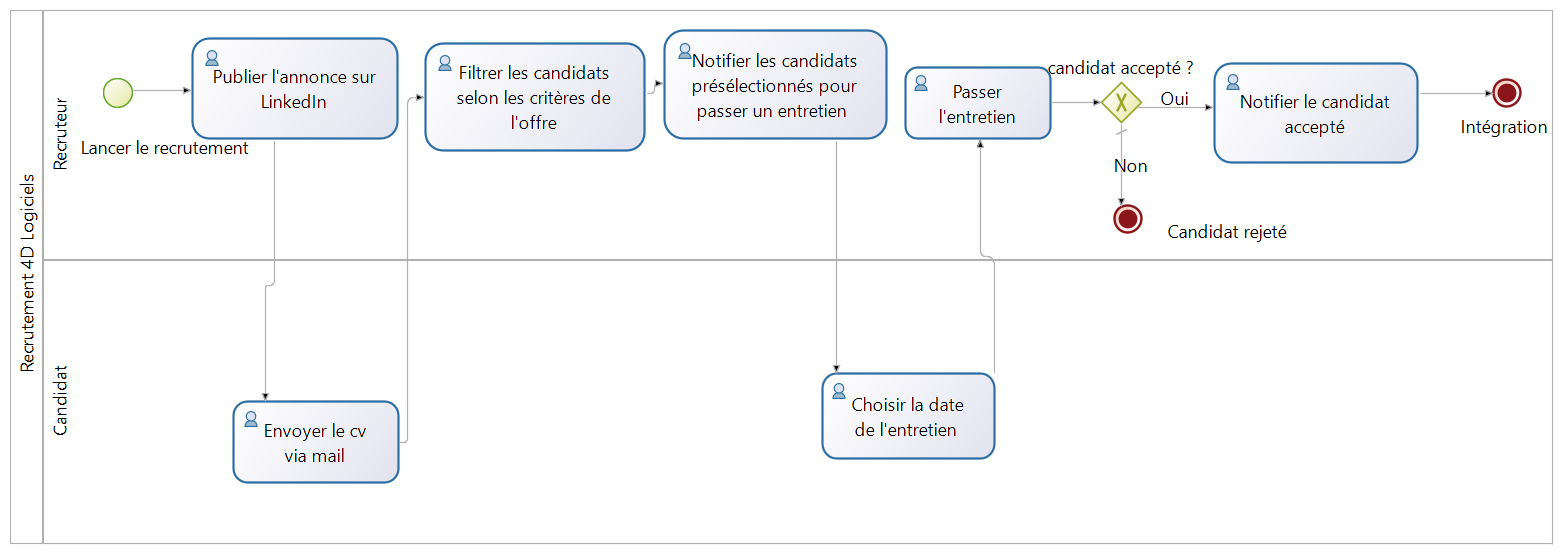
\includegraphics[scale=0.3]{Images/BPMN2.png} 
   \caption{Diagramme BPMN du processus actuel de recrutement chez 4D}
   \label{fig:BPMN1}
\end{figure}




%--------- Benchmarking ----------

\section{Benchmarking des principales solutions de recrutement}

Il existe une multitude de plateformes qui sont destinées à la gestion de recrutement
et qui proposent une variété de fonctionnalités facilitant ce processus. Parmi ces plateformes, nous citons :


{\small % Début de la taille de police small
\renewcommand{\arraystretch}{1.5}
\begin{longtable}{|p{2cm}|p{4.5cm}|p{4cm}|p{4.2cm}|}
\caption{Comparaison des solutions de recrutement} \\
\hline
\rowcolor{blue!30}
\textbf{Solution} & \textbf{Fonctionnalités principales} & \textbf{Avantages} & \textbf{Inconvénients} \\
\hline
\textbf{Indeed} & 
\begin{minipage}[t]{5cm}
- Publication d'offres \\ 
d'emploi \\
- Recherche de CV \\
- Campagnes sponsorisées\\
\end{minipage} &
\begin{minipage}[t]{5cm}
- Grande popularité \\
- Facilité d'utilisation
\end{minipage} &
\begin{minipage}[t]{5cm}
- Qualité variable\\
 des candidats \\
- Options limitées sans\\ 
paiement
\end{minipage} \\
\hline
\textbf{LinkedIn Recruiter} & 
\begin{minipage}[t]{5cm}
- Recherche avancée \\ 
de candidats \\
- Gestion des talents \\
- Analyses et rapports\\
\end{minipage} &
\begin{minipage}[t]{5cm}
- Large base de \\
données de candidats \\
- Outils de sourcing \\ 
puissants
\end{minipage} &
\begin{minipage}[t]{5cm}
- Coût élevé \\
- Complexité d'utilisation\\ 
pour les débutants
\end{minipage} \\
\hline
\textbf{Rekrute} & 
\begin{minipage}[t]{5cm}
- Publication d'offres \\ 
d'emploi \\
- Base de données de CV \\
- Solutions RH intégrées
\end{minipage} &
\begin{minipage}[t]{5cm}
- Forte présence en \\
Afrique du Nord \\
- Interface adaptée\\ 
aux marchés locaux
\end{minipage} &
\begin{minipage}[t]{6cm}
% - Moins connu en dehors \\ 
% des marchés ciblés \\
- Options limitées pour \\
les entreprises \\
multinationales\\
\\
\end{minipage} \\
\hline
\textbf{Odoo:  Module de recrutement} & 
\begin{minipage}[t]{5cm}
- Suivi des candidatures \\
- Intégration avec autres \\ 
modules Odoo \\
- Personnalisation des \\
processus de recrutement
\end{minipage} &
\begin{minipage}[t]{5cm}
- Intégration complète\\ 
avec l'écosystème Odoo \\
- Grande flexibilité \\ 
et personnalisation
\end{minipage} &
\begin{minipage}[t]{5cm}
- Complexité de \\ 
configuration initiale \\
- Nécessite des \\ 
compétences techniques \\ 
pour la personnalisation\\
\end{minipage} \\
\hline
\end{longtable}
} % Fin de la taille de police small


% Cette étude comparative nous a conduits à remarquer clairement 
% l'insuffisance des différentes solutions de recrutement disponibles 
% sur le marché. Certaines répondent aux besoins fonctionnels liés 
% seulement aux modules administratifs, et d’autres présentent des 
% complexités liées au déploiement et à l’installation. De plus, 
% la plupart des solutions sont fermées à l’introduction de nouvelles 
% fonctionnalités, révélant une absence totale de l’aspect évolutif des 
% systèmes.

% Après avoir étudié le marché du recrutement en ligne et 
% réalisé une étude comparative des différentes solutions 
% existantes qui a montré la limite de ces solutions par rapport aux besoins de l'entreprise,
% d'où la nécessité de 
% développer une plateforme 
% de recrutement interne chez 4D
Cette étude comparative met en évidence les lacunes des solutions de recrutement actuellement disponibles 
sur le marché. Certaines se limitent aux besoins fonctionnels des modules administratifs, tandis que d'autres 
présentent des complexités liées au déploiement et à l'installation. De plus, la plupart des solutions sont peu 
adaptables aux nouvelles fonctionnalités, révélant un manque d'évolutivité des systèmes existants.
En réponse à ces constats, il est nécessaire de développer une plateforme de recrutement interne chez 4D
 avec les éléments suivants : \\
% il est intéréssant de penser à 
% une solution interne avec un aspect 
% modulaire, évolutif et centralisé

\begin{spacing}{1.1}
\begin{itemize}
   \item[ • ] \textbf{Publication des offres d'emploi :} Permet une visibilité et un contrôle sur les annonces.
   \item[ • ] \textbf{Filtrage des CVs :} Facilite la sélection automatique des candidats en comparant leurs compétences avec celles requises pour le poste souhaité. 
   \item[ • ] \textbf{Passage de tests en ligne :}  Intégration de tests au sein de la plateforme pour évaluer les compétences des candidats de manière automatisée.
   \item[ • ] \textbf{Gestion complète du processus de recrutement :}  De la publication des offres à la planification des entretiens et la validation du candidat, chaque étape serait centralisée et automatisée. 
\end{itemize} 
\end{spacing}
% \vspace{2cm}
\section{Identification des acteurs}

% Un acteur est une entité externe jouant un rôle spécifique dans l'interaction avec le système. Les acteurs peuvent consulter et/ou modifier l'état du système en envoyant ou en recevant des messages contenant des données. Cette section vise à identifier les différents acteurs impliqués dans le système de recrutement, afin de mieux comprendre leurs interactions et leurs besoins spécifiques.

Dans le cadre de cette étude, différents acteurs jouent des rôles 
distincts dans le processus de recrutement. Un acteur est une entité 
externe qui interagit avec le système en assumant un rôle spécifique. 
Ces acteurs peuvent consulter et/ou modifier l'état du système en 
envoyant ou en recevant des messages contenant des données. Les principaux 
acteurs identifiés sont les candidats, les recruteurs et les 
administrateurs.

\renewcommand{\arraystretch}{1.5}
\begin{table}[htbp]
   \centering
   \caption{Rôles des Acteurs}
   \begin{tabular}{|p{3cm}|p{9cm}|}
       \hline
       \rowcolor{blue!30}
       \textbf{Acteur} & \textbf{Rôle} \\
       \hline
       Candidat & Il peut créer son profil, explorer les offres, postuler à celles-ci et suivre l’état d’avancement de sa candidature. \\
       \hline
       Recruteur & Chargé de gérer le processus de recrutement du début à la fin ; cela inclut la publication des offres d’emploi sur la plateforme, l'examen des candidatures reçues et la sélection des profils les plus pertinents pour organiser les entretiens avec les candidats. \\
       \hline
       Administrateur & Responsable de la gestion des utilisateurs, et il peut visualiser les Statistiques liées à la plateforme. \\
       \hline
   \end{tabular}
\end{table}

\section{Identification des besoins}

% Dans cette partie, notre objectif est de définir les fonctionnalités essentielles du système de recrutement digitalisé et son interaction avec l'environnement existant. 
% Afin de préciser les objectifs du projet, il est crucial de répondre à deux questions fondamentales : qui utilisera ce système et quelles sont leurs attentes ? Pour y parvenir, nous avons suivi les étapes suivantes : \\

% \begin{itemize}
%    \item[ • ] Identifier les différents utilisateurs du système de recrutement.
%    \item[ • ] Énumérer les fonctionnalités nécessaires que le système doit offrir à ces utilisateurs.\\

% \end{itemize}

% En procédant ainsi, nous pouvons déterminer les besoins spécifiques des
%  diverses parties prenantes et nous assurer que le système de recrutement 
%  répondra de manière efficace aux attentes de 4D Logiciels. Les 
%  spécifications des exigences permettront de développer une solution 
%  qui facilite la gestion des candidatures, améliore la précision du 
%  filtrage, centralise les informations des candidats et optimise la 
%  coordination des entretiens.



\subsection{Besoins fonctionnels}
Afin d’atteindre les objectifs souhaités, il est important d’identifier avec 
précision les besoins fonctionnels du système. 
% Les besoins fonctionnels sont
% les besoins fonctionnels du projet. Les différentes réunions 
% avec l'encadrant (représentant métier) ont permis de spécifier en détail les exigences
% fonctionnelles que la solution doit satisfaire. 
L’ensemble de la solution doit 
répondre aux spécifications fonctionnelles suivantes :
\\
\begin{itemize}
    \setlength{\itemsep}{0.3cm}
   \item[•] \textbf{Authentification} :
   \begin{itemize}
    \setlength{\itemsep}{0.2cm}
       \item[-] Les utilisateurs peuvent se connecter à la plateforme en utilisant leurs identifiants personnels (email/mot de passe).
   \end{itemize}
   \item[•] \textbf{Gestion des offres d'emploi} :
   \begin{itemize}
    \setlength{\itemsep}{0.2cm}
       \item[-] Permettre aux recruteurs de créer, modifier et supprimer des offres d'emploi en spécifiant les détails tels que le titre du poste, les responsabilités, les compétences requises, la localisation, etc.
   \end{itemize}
   
   \item[•] \textbf{Analyse des CVs} :
   \begin{itemize}
    \setlength{\itemsep}{0.2cm}
       \item[-] Extraire automatiquement les informations clés des CVs des candidats, comme les compétences, l'expérience professionnelle, l'éducation, etc.
       \item[-] Comparer les informations extraites des CVs avec les critères définis dans l'offre d'emploi pour évaluer la pertinence de chaque candidature.
   \end{itemize}
   
   \item[•] \textbf{Tests en ligne} :
   \begin{itemize}
    \setlength{\itemsep}{0.2cm}
       \item[-] Permettre aux candidats de passer des tests d'aptitude ou des évaluations techniques directement sur la plateforme.
   \end{itemize}
   
   \item[•] \textbf{Planification des entretiens en ligne} :
   \begin{itemize}
    \setlength{\itemsep}{0.2cm}
       \item[-] Permettre aux recruteurs de planifier des entretiens en ligne 
       en fonction de leurs disponibilités, 
       en affichant les créneaux horaires disponibles dans un 
       calendrier intégré.
   \end{itemize}
   
   \item[•] \textbf{Gestion des calendriers} :
   \begin{itemize}
    \setlength{\itemsep}{0.2cm}
       \item[-] Intégrer un système de gestion de calendrier permettant aux 
       candidats et aux recruteurs de visualiser et de gérer leurs 
       rendez-vous pour les entretiens.
       \item[-] Envoyer des rappels automatiques aux candidats et aux recruteurs pour leurs rendez-vous programmés.
   \end{itemize}
   
   \item[•] \textbf{Suivi des candidatures} :
   \begin{itemize}
    \setlength{\itemsep}{0.2cm}
       \item[-] Fournir aux candidats une interface pour suivre l'état 
       de chaque candidature, de la soumission initiale jusqu'à la 
       décision finale de recrutement.
       \item[-] Permettre aux recruteurs de voir les différents candidats 
       qui ont postulé à une offre.
   \end{itemize}
   
   \item[•] \textbf{Statistiques} :
   \begin{itemize}
    \setlength{\itemsep}{0.2cm}
    %    \item[-] Générer des rapports personnalisés pour les recruteurs, fournissant des données telles que le nombre de candidatures par offre, le taux de réussite aux tests, le délai moyen de recrutement, etc.
       \item[-] Visualiser des graphiques et des tableaux de bord pour analyser les tendances de recrutement et identifier les domaines d'amélioration.
   \end{itemize}
   
   \item[•] \textbf{Gestion des utilisateurs} :
   \begin{itemize}
    \setlength{\itemsep}{0.2cm}
       \item[-] L'administrateur de l'application a le pouvoir de gérer les comptes utilisateurs.
       
   \end{itemize}
\end{itemize}



\subsection{Besoins non fonctionnels}

Ces besoins représentent les 
contraintes auxquelles le système est soumis pour sa réalisation et son bon 
fonctionnement. Ils doivent être pris en compte tout au long du développement 
du projet afin de garantir la performance du produit final et de satisfaire les 
exigences de 4D Logiciels. Les contraintes suivantes ont 
été identifiées :

\begin{itemize}
    \setlength{\itemsep}{0.3cm}
    \item[•] \textbf{ Sécurité des Données :}
    \begin{itemize}
        \setlength{\itemsep}{0.2cm}
        \item[-] Mettre en place des mesures de sécurité robustes pour protéger les 
        données sensibles des candidats et des recruteurs, en utilisant le 
        chiffrement des données, l'authentification sécurisée, etc.        
    \end{itemize}
    \item[•] \textbf{Performance :}
    \begin{itemize}
        \setlength{\itemsep}{0.2cm}
        \item[-]Optimiser les performances de la plateforme pour assurer des temps 
        de chargement rapides et une navigation fluide, même lorsqu'il y a 
        un grand nombre d'utilisateurs actifs simultanément.
        % \item[-] Mettre en place des serveurs robustes et une architecture évolutive 
        % pour gérer la montée en charge lors de pics d'activité.
    \end{itemize}
    \item[•] \textbf{Disponibilité :}
    \begin{itemize}
        \setlength{\itemsep}{0.2cm}
        \item[-] Assurer une disponibilité du système pour garantir un accès 
        continu aux utilisateurs, minimisant ainsi les interruptions de service 
        et les temps d'arrêt imprévus.\\

    \end{itemize}
    \item[•] \textbf{Évolutivité :}
    \begin{itemize}
        \setlength{\itemsep}{0.2cm}
        \item[-] Concevoir une architecture modulaire et évolutive permettant 
        d'ajouter de nouvelles fonctionnalités et de s'adapter aux besoins évolutifs 
        de l'entreprise et des utilisateurs.
        % \item[-] Prévoir des mises à jour régulières et des améliorations continues pour garantir la pertinence et la compétitivité de la plateforme dans le temps.
    \end{itemize}
\end{itemize}


\section{Diagramme de cas d’utilisation}

% Les diagrammes de cas d’utilisation sont essentiels pour 
% structurer les besoins des différents acteurs et les fonctionnalités 
% offertes par le système. Ils mettent l'accent sur l'expression des 
% exigences en se concentrant sur les acteurs. La détermination et 
% la compréhension des besoins sont souvent complexes, car les 
% intervenants sont submergés par une quantité importante 
% d'informations. Il est donc nécessaire de clarifier et d'organiser 
% ces besoins, c’est-à-dire de les modéliser.
Le diagramme de cas d'utilisation structure les besoins des acteurs 
et les fonctionnalités du système. Il clarifie et organise 
ces besoins en se concentrant sur les intéractions des acteurs avec 
le système, facilitant ainsi la compréhension et la modélisation 
des exigences.
% Les cas d’utilisation 
% permettent d’identifier les acteurs du système et leurs interactions 
% avec celui-ci, classant ainsi les acteurs et structurant les 
% objectifs du système.
\subsection{Diagramme de cas d’utilisation du candidat}
Ce diagramme illustre les interactions principales entre le 
candidat et les différentes fonctionnalités de la plateforme. 

\begin{figure}[h]
    \centering
    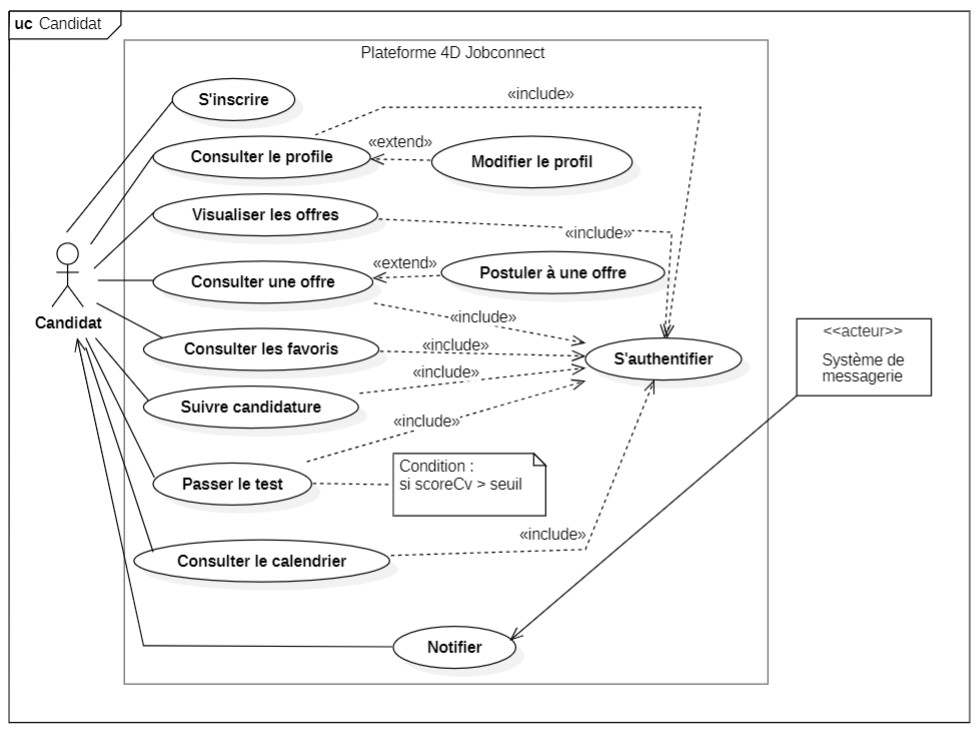
\includegraphics[scale=1]{Images/Candidat1.jpg} % Replace with the actual filename of the IBM logo image
    \caption{Diagramme de cas d’utilisation du candidat}
    \label{fig:UCCandidat}
\end{figure}
\vspace{8cm}

\subsection{Diagramme de cas d’utilisation du recruteur}
Ce diagramme illustre les interactions principales entre le 
recruteur et les différentes fonctionnalités de la plateforme
\begin{figure}[h]
    \centering
    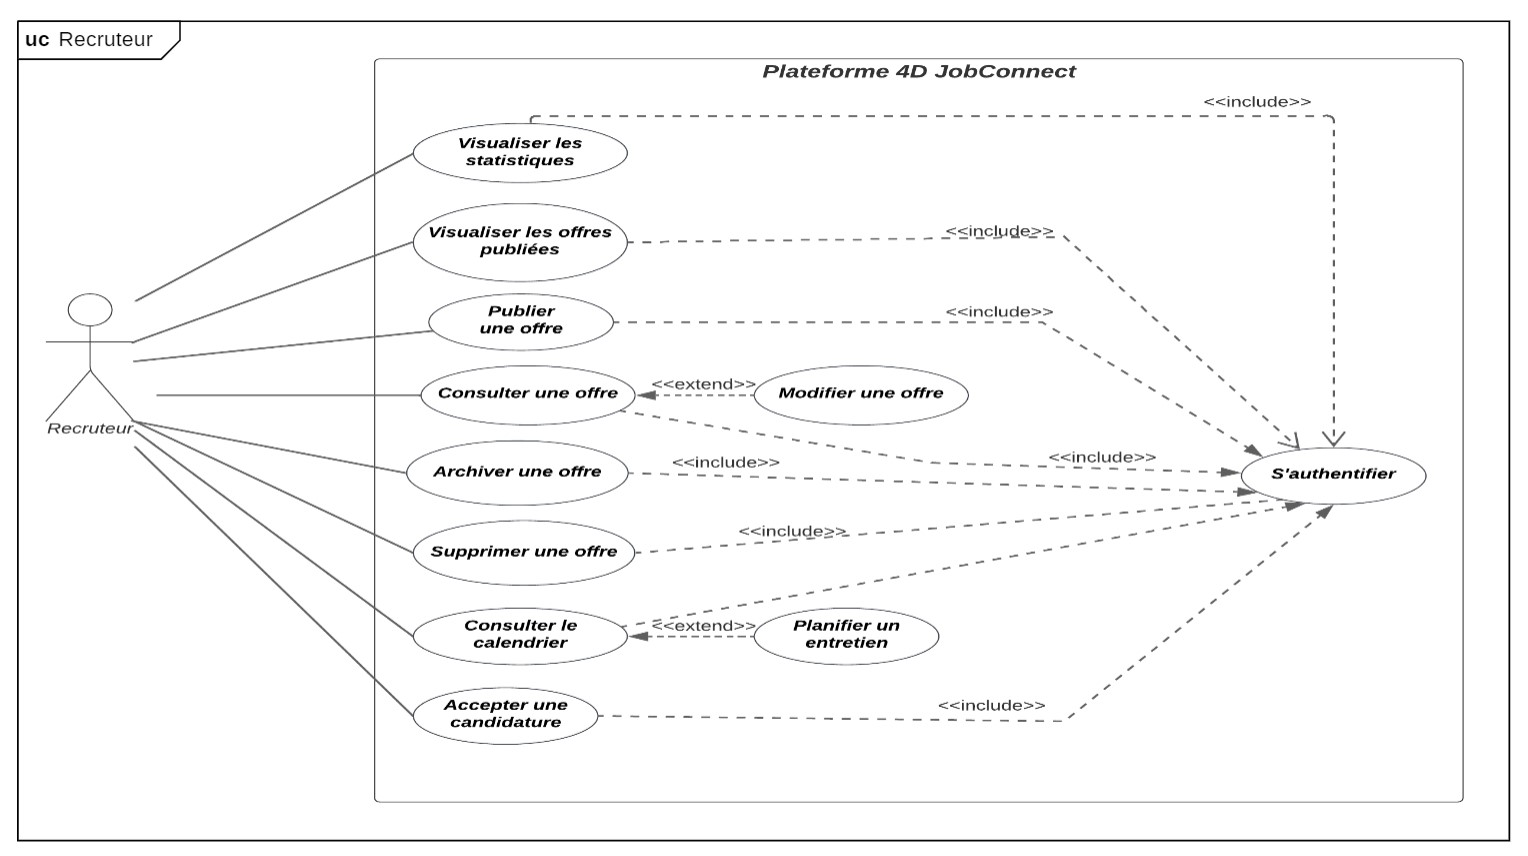
\includegraphics[scale=0.67]{Images/recruteur.jpg} % Replace with the actual filename of the IBM logo image
    \caption{Diagramme de cas d’utilisation du recruteur}
    \label{fig:UCRecruteur}
\end{figure}
\vspace{12cm}

\subsection{Diagramme de cas d’utilisation de l'administrateur}
Ce diagramme illustre les interactions principales entre le 
l’administrateur et les différentes fonctionnalités de la plateforme
\begin{figure}[htbp]
    \centering
    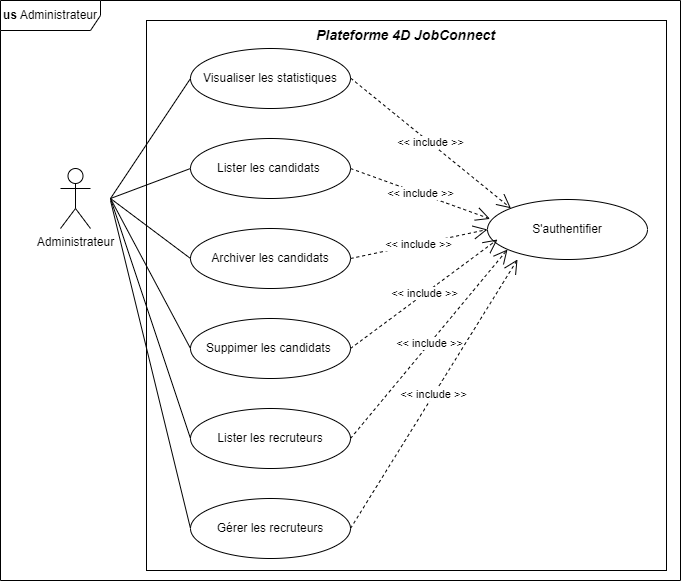
\includegraphics[scale=0.7]{diag/adminUC.png} % Replace with the actual filename of the IBM logo image
    \caption{Diagramme de cas d’utilisation de l'administrateur}
    \label{fig:UCAdmin}
\end{figure}
\vspace{1cm}

% Description textuelle
\section{Description textuelle des cas d'utilisation}

Afin de mieux décrire le comportement du système, il est recommandé 
d'utiliser la description textuelle des cas d’utilisation. 
Cette approche permet de détailler de manière claire et structurée 
les interactions entre les acteurs et le système.

\subsection{Description textuelle : Publier une offre}
\begin{minipage}{\textwidth}
    \begin{table}[H]
    \centering
    \caption{Description Textuelle du Cas d'Utilisation "Publier une offre par le recruteur"}
    \begin{tabular}{| m{8cm} | m{8cm} |}
    \hline
    \multicolumn{2}{|c|}{\textbf{UC 1:} Publier une offre par le recruteur} \\ \hline
    \textbf{Acteur} & Recruteur \\ \hline
    \textbf{But} & Permettre à un recruteur de publier une nouvelle offre d'emploi sur la plateforme. \\ \hline
    \textbf{Préconditions} & \textbf{Postconditions} \\ \hline
    - Être authentifié en tant que recruteur. & - Une nouvelle offre est publiée sur la plateforme. \\ \hline
    \textbf{Scénario Principal} & \textbf{Scénario Alternatif} \\ \hline
    \begin{enumerate}
        \item Se connecter en tant que recruteur.
        \item Accéder à l'interface de publication des offres.
        \item Remplir les informations de l'offre : titre, description, compétences requises, localisation, etc.
        \item Publier l'offre sur la plateforme.
    \end{enumerate} & 
    \begin{enumerate}
        \item Le recruteur rencontre un problème de connexion.
        \item Le recruteur ne remplit pas tous les champs obligatoires.
        \item La publication de l'offre échoue en raison d'une erreur technique.
    \end{enumerate} \\ \hline
    \end{tabular}
    \label{tab:UCPublier_Offre}
    \end{table}
\end{minipage}

\subsection{Description textuelle : Postuler à une offre}

\begin{minipage}{\textwidth}
    \begin{table}[H]
    \centering
    \caption{Description Textuelle du Cas d'Utilisation "Postuler à une offre par le candidat"}
    \begin{tabular}{| m{8cm} | m{8cm} |}
    \hline
    \multicolumn{2}{|c|}{\textbf{UC 2:} Postuler à une offre par le candidat} \\ \hline
    \textbf{Acteurs} & Candidat \\ \hline
    \textbf{But} & Permettre à un candidat de postuler à une offre d'emploi disponible sur la plateforme. \\ \hline
    \textbf{Préconditions} & \textbf{Postconditions} \\ \hline
    - Être authentifié en tant que candidat. & - La candidature est soumise avec succès. \\ 
    - Documents requis téléversés dans le profil. & \\ \hline
    \textbf{Scénario Principal} & \textbf{Scénario Alternatif} \\ \hline
    \begin{enumerate}
        \item Se connecter en tant que candidat.
        \item Consulter les offres d'emploi disponibles.
        \item Sélectionner une offre qui correspond à ses compétences et intérêts.
        \item Cliquer sur le bouton "Postuler".
        \item Télécharger et soumettre les documents requis.
    \end{enumerate} & 
    \begin{enumerate}
        \item Problème de connexion.
        \item Aucune offre ne correspond à ses critères.
        \item Les documents requis ne sont pas téléversés :
            \begin{enumerate}
                \item Redirection vers la page de modification du profil pour téléverser les documents.
            \end{enumerate}
        \item Erreur technique lors de la soumission de la candidature.
    \end{enumerate} \\ \hline
    \end{tabular}
    \label{tab:UCPostuler_Offre}
    \end{table}
\end{minipage}

\subsection{Description textuelle : Passer le test}
\begin{minipage}{\textwidth}
    \begin{table}[H]
    \centering
    \caption{Description Textuelle du Cas d'Utilisation "Passer le test"}
    \begin{tabular}{| m{8cm} | m{8cm} |}
    \hline
    \multicolumn{2}{|c|}{\textbf{UC 3:} Passer le test} \\ \hline
    \textbf{Acteurs} & Candidat \\ \hline
    \textbf{But} & Permettre à un candidat de passer un test en ligne lié à une offre d'emploi. \\ \hline
    \textbf{Préconditions} & \textbf{Postconditions} \\ \hline
    - Avoir un score de CV supérieur au seuil défini.\\
    - Avoir déjà postulé à l'offre correspondante. & - Le test est passé avec succès. \\ \hline
    \textbf{Scénario Principal} & \textbf{Scénario Alternatif} \\ \hline
    \begin{enumerate}
        \item Être authentifié en tant que candidat.
        \item Consulter les offres d'emploi deja postulé
        \item Sélectionner une offre à laquelle le candidat a déjà postulé.
        \item Cliquer sur le bouton "Passer le test".
        \item Répondre aux questions du test en ligne.
        \item Soumettre les réponses.
    \end{enumerate} & 
    \begin{enumerate}
        \item Score de CV inférieur au seuil.
        \item Le candidat n'a pas encore postulé à l'offre correspondante.
        \item Problème technique lors du passage du test.
    \end{enumerate} \\ \hline
    \end{tabular}
    \label{tab:UCPasser_Test}
    \end{table}
\end{minipage}


% \section{Conclusion}
% Ce chapitre aborde une phase essentielle pour l'étude et l'analyse 
% de notre application. Nous y avons défini les différents besoins 
% fonctionnels et non fonctionnels, présenté les diagrammes de cas 
% d’utilisation, ainsi que leurs descriptions textuelles. Le chapitre 
% suivant se concentrera sur la conception de notre solution en 
% s'appuyant sur la concecption des maquettes, la détermination de 
% l'architecture de notre système, et la modélisation des diagrammes de séquence et des diagrammes de 
% classes.


\section{Conclusion}
Ce chapitre a analysé en profondeur le processus de recrutement 
actuel chez 4D, révélant des lacunes importantes dues à 
l'utilisation d'outils fragmentés et à une forte intervention 
manuelle, entraînant des risques de perte d'information et des 
inefficacités. L'étude comparative des solutions de recrutement 
disponibles a démontré leur incapacité à satisfaire pleinement 
les besoins spécifiques de l'entreprise, soulignant la nécessité 
de développer une plateforme interne, moderne et modulaire. 
Nous avons spécifié les besoins fonctionnels et non fonctionnels 
de cette solution, défini les rôles des différents acteurs et 
détaillé les cas d'utilisation pertinents, établissant ainsi 
une base pour la conception et le développement de la 
nouvelle plateforme de recrutement, que nous allons détailler 
au niveau des chapitres suivants.
% Define the page style
\fancypagestyle{chapterstyle}{
   \fancyhead[L]{\nouppercase{\rightmark}}
   \fancyhead[R]{Projet de fin d'etudes 2023-2024}
   \fancyfoot[C]{\vspace{20pt}\thepage} % Adjust the vertical space here
   \setlength{\headheight}{20pt}
   \setlength{\footskip}{30pt} % Adjust the value as needed
}


\chapter{Conception de la solution}
\pagestyle{chapterstyle}

\newpage
\vspace{1cm}

\section{Introduction}
% Ce chapitre détaille la conception de notre solution. Après avoir défini les 
% besoins et les cas d'utilisation, nous utiliserons des maquettes 
% pour visualiser l'interface utilisateur, des diagrammes de séquence 
% pour illustrer les interactions dynamiques entre les composantes 
% de l'application et des diagrammes de classes pour structurer les 
% éléments et leurs relations. Cette étape assure une mise en œuvre 
% cohérente et efficace, intégrant toutes les exigences identifiées.
% Ce chapitre détaille la conception de notre solution. 
% Après avoir spécifié les besoins, nous avons mis en place des maquettes pour bien illustrer ces besoins. 
% Puis dans le cadre d'une conception générale,
% nous avons conçu une architecture pour notre solution. 
% Par la suite, nous avons conçu le diagramme de classe 
% et les diagrammes de séquence.

Ce chapitre détaille la conception de notre solution. Après avoir spécifié 
les besoins, nous avons créé des maquettes pour illustrer 
ces exigences. Ensuite, dans le cadre d'une conception générale, nous avons 
élaboré une architecture pour notre solution. Par la suite, nous avons 
conçu le diagramme de classes ainsi que les diagrammes de séquence.


\section{Maquettes}
Le design UX/UI est un élément principal de notre projet, 
car il vise à aligner les objectifs du client (entreprise 4D) et ses attentes avec 
le travail qui va être réalisé par la suite.
\newline
Dans notre situation, nous avons converti les besoins fonctionnels du système 
en maquettes. Cela nous a permis de préparer l'interface globale 
avant d'entrer dans la phase de développement. Ensuite, 
nous avons sollicité les retours du client 
afin d'améliorer encore notre application.
\newline
% \vspace{4cm}



\begin{figure}[htbp]
   \centering
   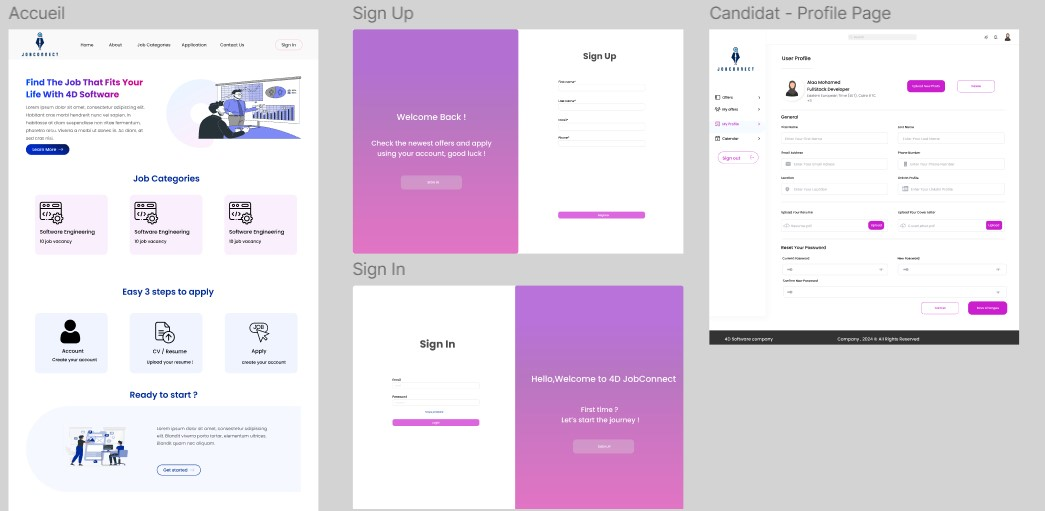
\includegraphics[scale=0.8]{Images/1.jpg} % Replace with the actual filename of the IBM logo image
   \caption{Maquettes Authentification et Profile}
   \label{fig:maquette1}
\end{figure}
% \vspace{1cm}
\vspace{4cm}
\begin{figure}[htbp]
   \centering
   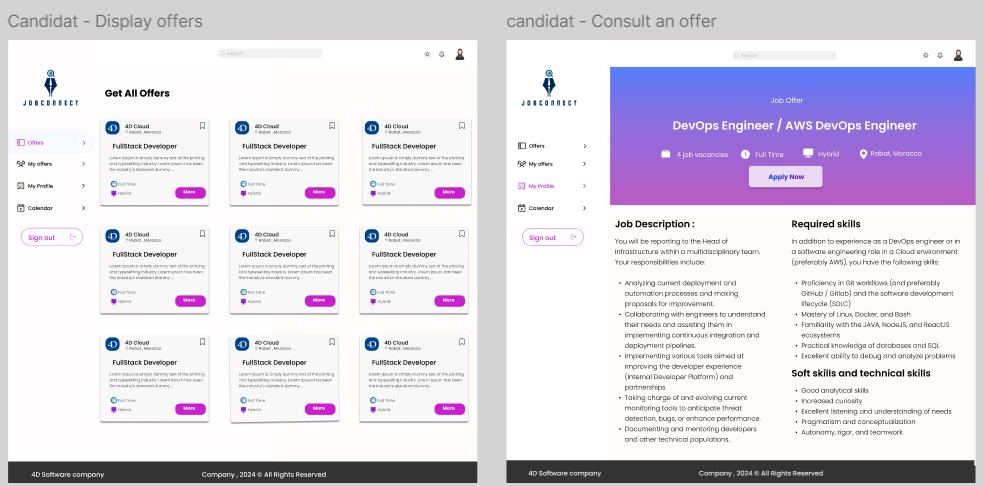
\includegraphics[scale=0.8]{Images/2.jpg} 
   \caption{Maquettes Offres}
   \label{fig:maquette2}
\end{figure}

\begin{figure}[htbp]
   \centering
   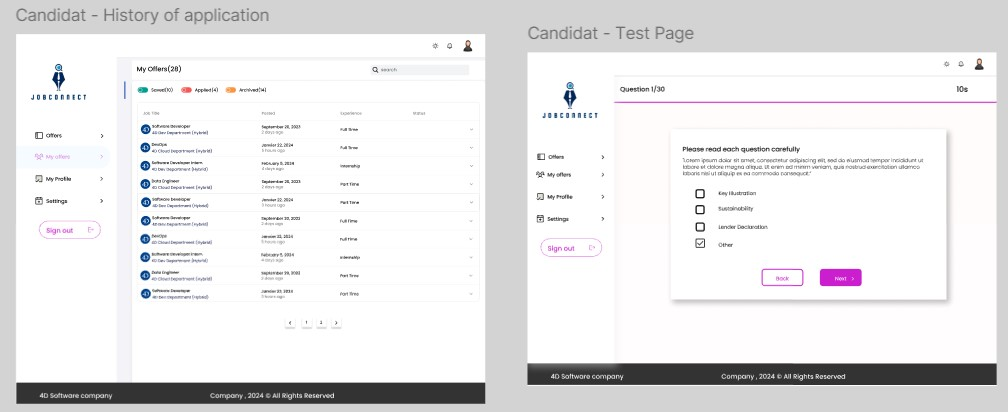
\includegraphics[scale=1]{Images/3.jpg} 
   \caption{Maquettes historique de candidature et test}
   \label{fig:maquette3}
\end{figure}

\begin{figure}[htbp]
   \centering
   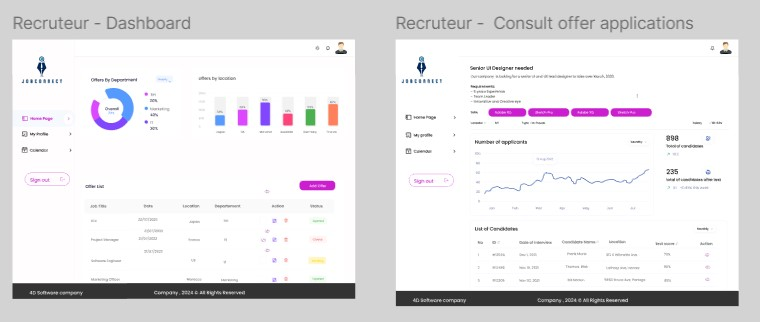
\includegraphics[scale=1.4]{Images/4.jpg} 
   \caption{Maquettes Dashboard recruteur}
   \label{fig:maquette4}
\end{figure}

\begin{figure}[htbp]
   \centering
   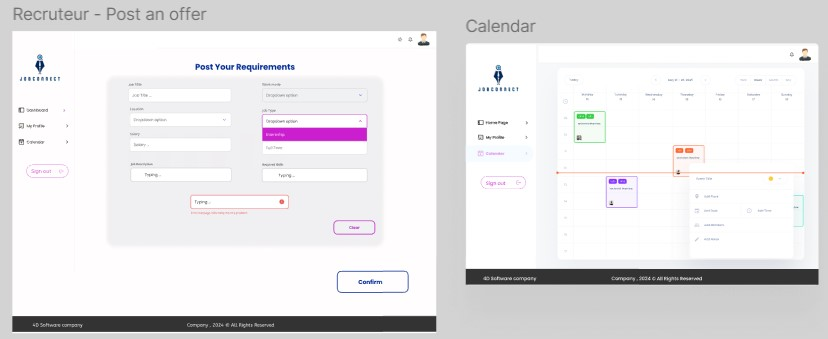
\includegraphics[scale=1.2]{Images/5.jpg} 
   \caption{Maquettes créer une offre et consulter calendrier}
   \label{fig:maquette5}
\end{figure}


\section{Architecture de l'application}
\subsection{Architecture physique}
% Notre application adopte une architecture client/serveur 
% multi-tiers. Ainsi, l'accès à 
% l'application nécessite le transit par des requêtes HTTP pour 
% récupérer et déposer les données dans le dépôt central. De plus, 
% nous avons centralisé la gestion de la base de données du système, 
% la séparant de la logique métier pour faciliter la maintenance. 
% Enfin, l'application est répartie sur plusieurs serveurs, chacun 
% responsable d'une tâche spécifique. Cette répartition des tâches 
% entre les serveurs permet d'assurer une grande souplesse, 
% des performances optimales et des temps de réponse rapides. 
Notre application adopte une architecture client/serveur multi-tiers. 
Les requêtes HTTP permettent de récupérer et déposer des données dans le dépôt 
central. La gestion de la base de données est centralisée et séparée de la 
logique métier pour faciliter la maintenance. L'application est répartie sur 
plusieurs serveurs, chacun responsable d'une tâche spécifique, assurant ainsi 
une rapidité de réponse.
La figure \ref{fig:physiqueArch} illustre l'architecture physique que nous avons mis en place :


\begin{figure}[htbp]
   \centering
   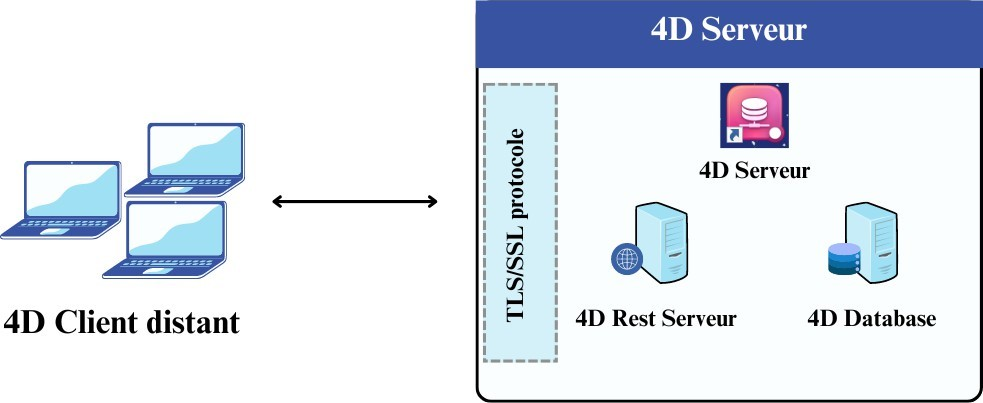
\includegraphics[scale=0.6]{Images/physique.jpg} % Replace with the actual filename of the IBM logo image
   \caption{Architecture physique}
   \label{fig:physiqueArch}
\end{figure}

Cette architecture se compose principalement des éléments suivants :
\begin{itemize}
   \item[•] \textbf{Serveur REST :} Un serveur web qui suit les principes de l’architecture REST et expose des ressources via des URIs, permettant aux clients d’effectuer des opérations standardisées sur ces ressources pour accéder aux données et fonctionnalités du serveur.
   \item[•] \textbf{Serveur 4D :} Ce serveur contient la couche métier de notre application.
   \item[•] \textbf{Serveur de base de données :} Ce serveur se charge de la gestion du stockage des données.
   \item[•] \textbf{Couche réseau :} Le protocole TLS sécurise les connexions client/serveur en cryptant les données échangées, permettant ainsi de renforcer la sécurité de l'application.
\end{itemize}

\subsection{Architecture logique}
Pour avoir une architecture robuste, modulable et évolutive, il faut utiliser le principe de « Couche », et donc séparer au maximum les différents types de traitement de l’ap- plication. L’environnement de travail n’est pas dépendant à une technologie spécifique. Pour cette raison, nous avons utilisé plusieurs technologies afin de développer une solu- tion aboutie, performante, multicouches et qui s’intègre parfaitement. La figure suivante illustre l’architecture logicielle proposée pour le système développé, en présentant trois couches : couche présentation (web), couche métier qui s’occupe des différents traitements et couche accès aux données.

\begin{figure}[htbp]
   \centering
   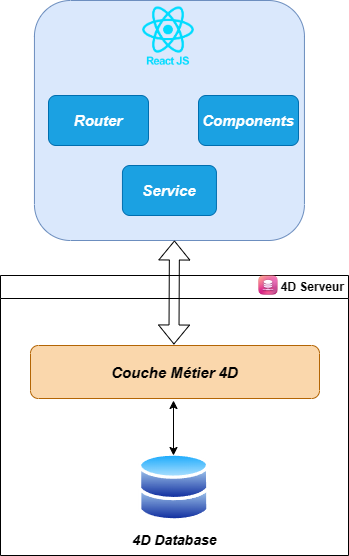
\includegraphics[scale=0.5]{Images/logi.png} 
   \caption{Architecture logique}
   \label{fig:logiqueArch}
\end{figure}

Au niveau 4D Server, notre développement s’est concentré principalement sur la couche métier. En effet, 4D Server offre un environnement de développement qui simplifie considérablement la création d’applications. Les autres couches, telles que la couche d’accès aux données et la couche de présentation, sont déjà implémentées et intégrées dans 4D.Ainsi, les développeurs peuvent se concentrer sur la logique métier de leurs applications sans avoir à se soucier des détails techniques des autres couches. Cette approche permet un développement rapide et efficace, tout en offrant des fonctionnalités avancées pour répondre aux besoins spécifiques des projets.
\newline

Ainsi, les développeurs peuvent se concentrer sur la logique métier de leurs applications sans avoir à se soucier des détails techniques des autres couches. Cette approche permet un développement rapide et efficace, tout en offrant des fonctionnalités avancées pour répondre aux besoins spécifiques des projets.
\newline

% Aussi, nous avons travaillé avec ORDA, est une technologie spécifique qui facilite l’accès à une base de données relationnelle en tant qu’objets. Elle permet de manipuler les données de la base de données à l’aide d’un langage de programmation orienté objet ou d’interfaces utilisateur spécifiques. ORDA simplifie l’interaction avec la base de données en fournissant des abstractions supplémentaires et en masquant certaines complexités liées aux requêtes SQL.
% ORDA nous permet de créer des fonctions de classe de haut niveau au-dessus du modèle de données. Cela nous permet d’écrire du code orienté métier et de le «publier» comme une API. Le datastore, les
% dataclasses, les entity selections et les entités sont tous disponibles en tant qu’objets de classe pouvant contenir des fonctions.
Aussi, nous avons travaillé avec ORDA, est une technologie spécifique qui facilite l’accès à une base de données relationnelle en tant qu’objets. Elle permet de manipuler les données de la base de données à l’aide d’un langage de programmation orienté objet ou d’interfaces utilisateur spécifiques. ORDA simplifie l’interaction avec la base de données en fournissant des abstractions supplémentaires et en masquant certaines complexités liées aux requêtes SQL.
\newline

% Grâce à 4D, les développeurs peuvent se concentrer sur l’essentiel et créer des appli- cations puissantes et performantes en toute simplicité.


% \begin{figure}[htbp]
%    \centering
%    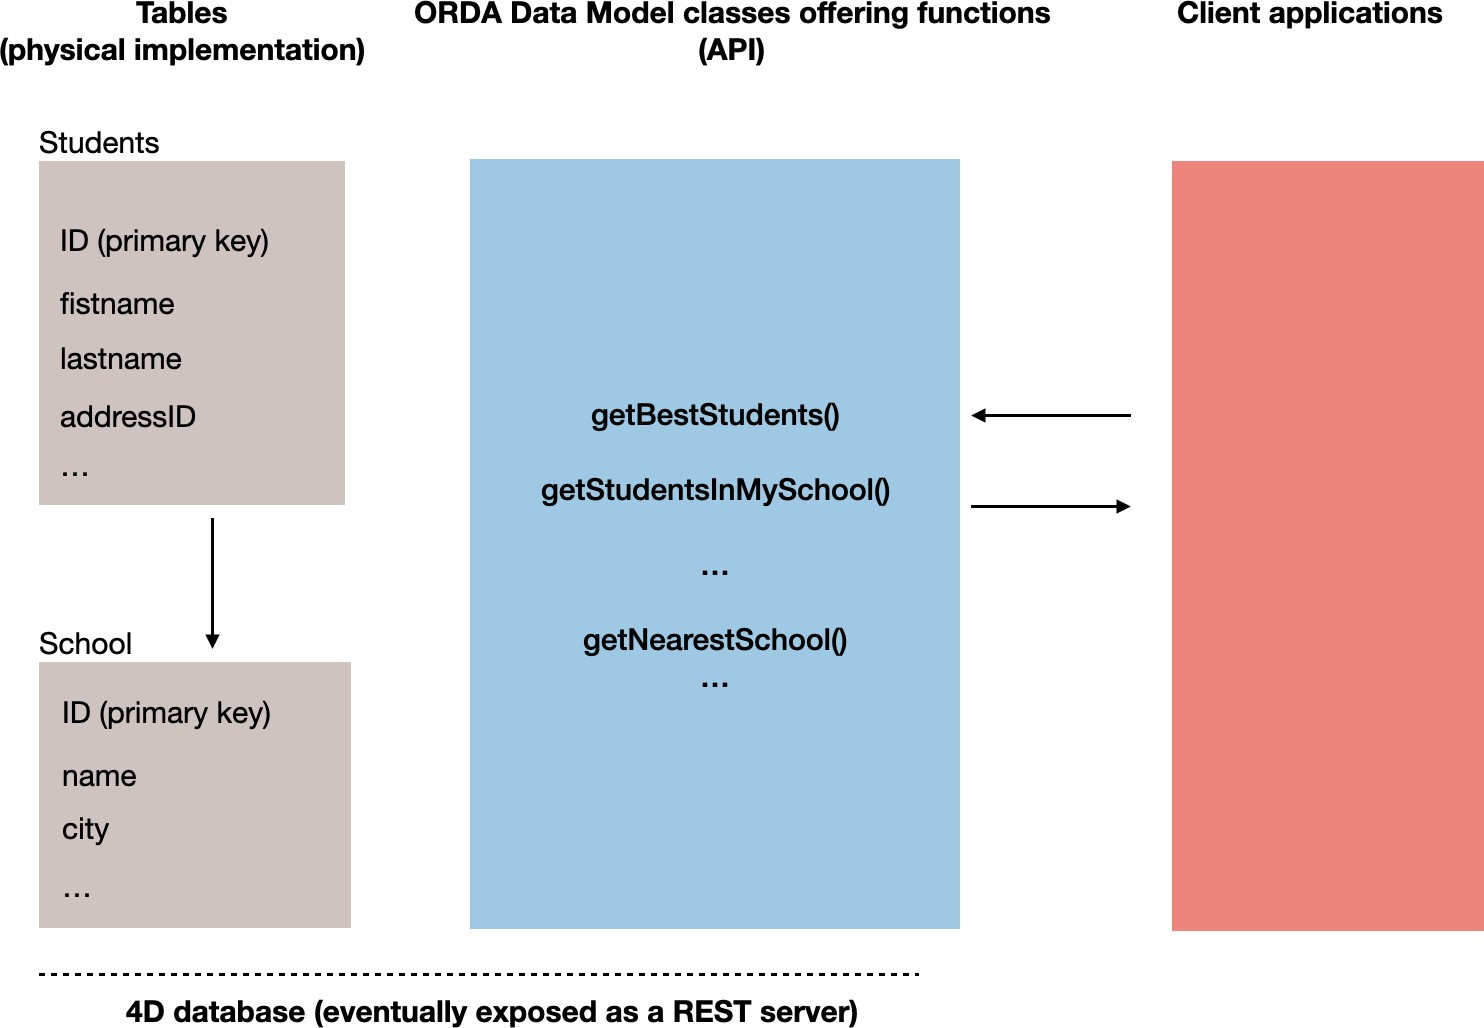
\includegraphics[scale=0.3]{Images/logique 2.jpg} 
%    \caption{Architecture logique}
%    \label{fig:logiqueArch}
% \end{figure}


% \subsection{Architecture technique}

% \begin{figure}[htbp]
%    \centering
%    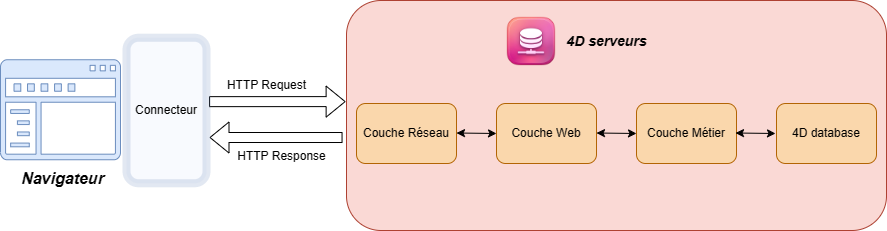
\includegraphics[scale=0.6]{Images/techn.png} % Replace with the actual filename of the IBM logo image
%    \caption{Architecture technique}
%    \label{fig:seq4}
% \end{figure}

% Le connecteur s’occupe de la récolte des données saisies par l’utilisateur dans le navi- gateur, ces données sont envoyées au serveur 4D via des requêtes HTTP. La couche web récupère les données reçues et les transmet à la couche métier qui effectue les traitements nécessaires. La couche 4D Database s’occupe de la sérialisation et la dé-sérialisation.

% \section{Conception détaillée}
\section{Diagramme de Classes}
Le diagramme de classes est l'un des diagrammes statiques d'UML. 
Il permet de représenter la structure d'un système informatique en 
présentant les différentes classes, leurs attributs, leurs méthodes, 
ainsi que les relations entre elles.

\begin{figure}[htbp]
   \centering
   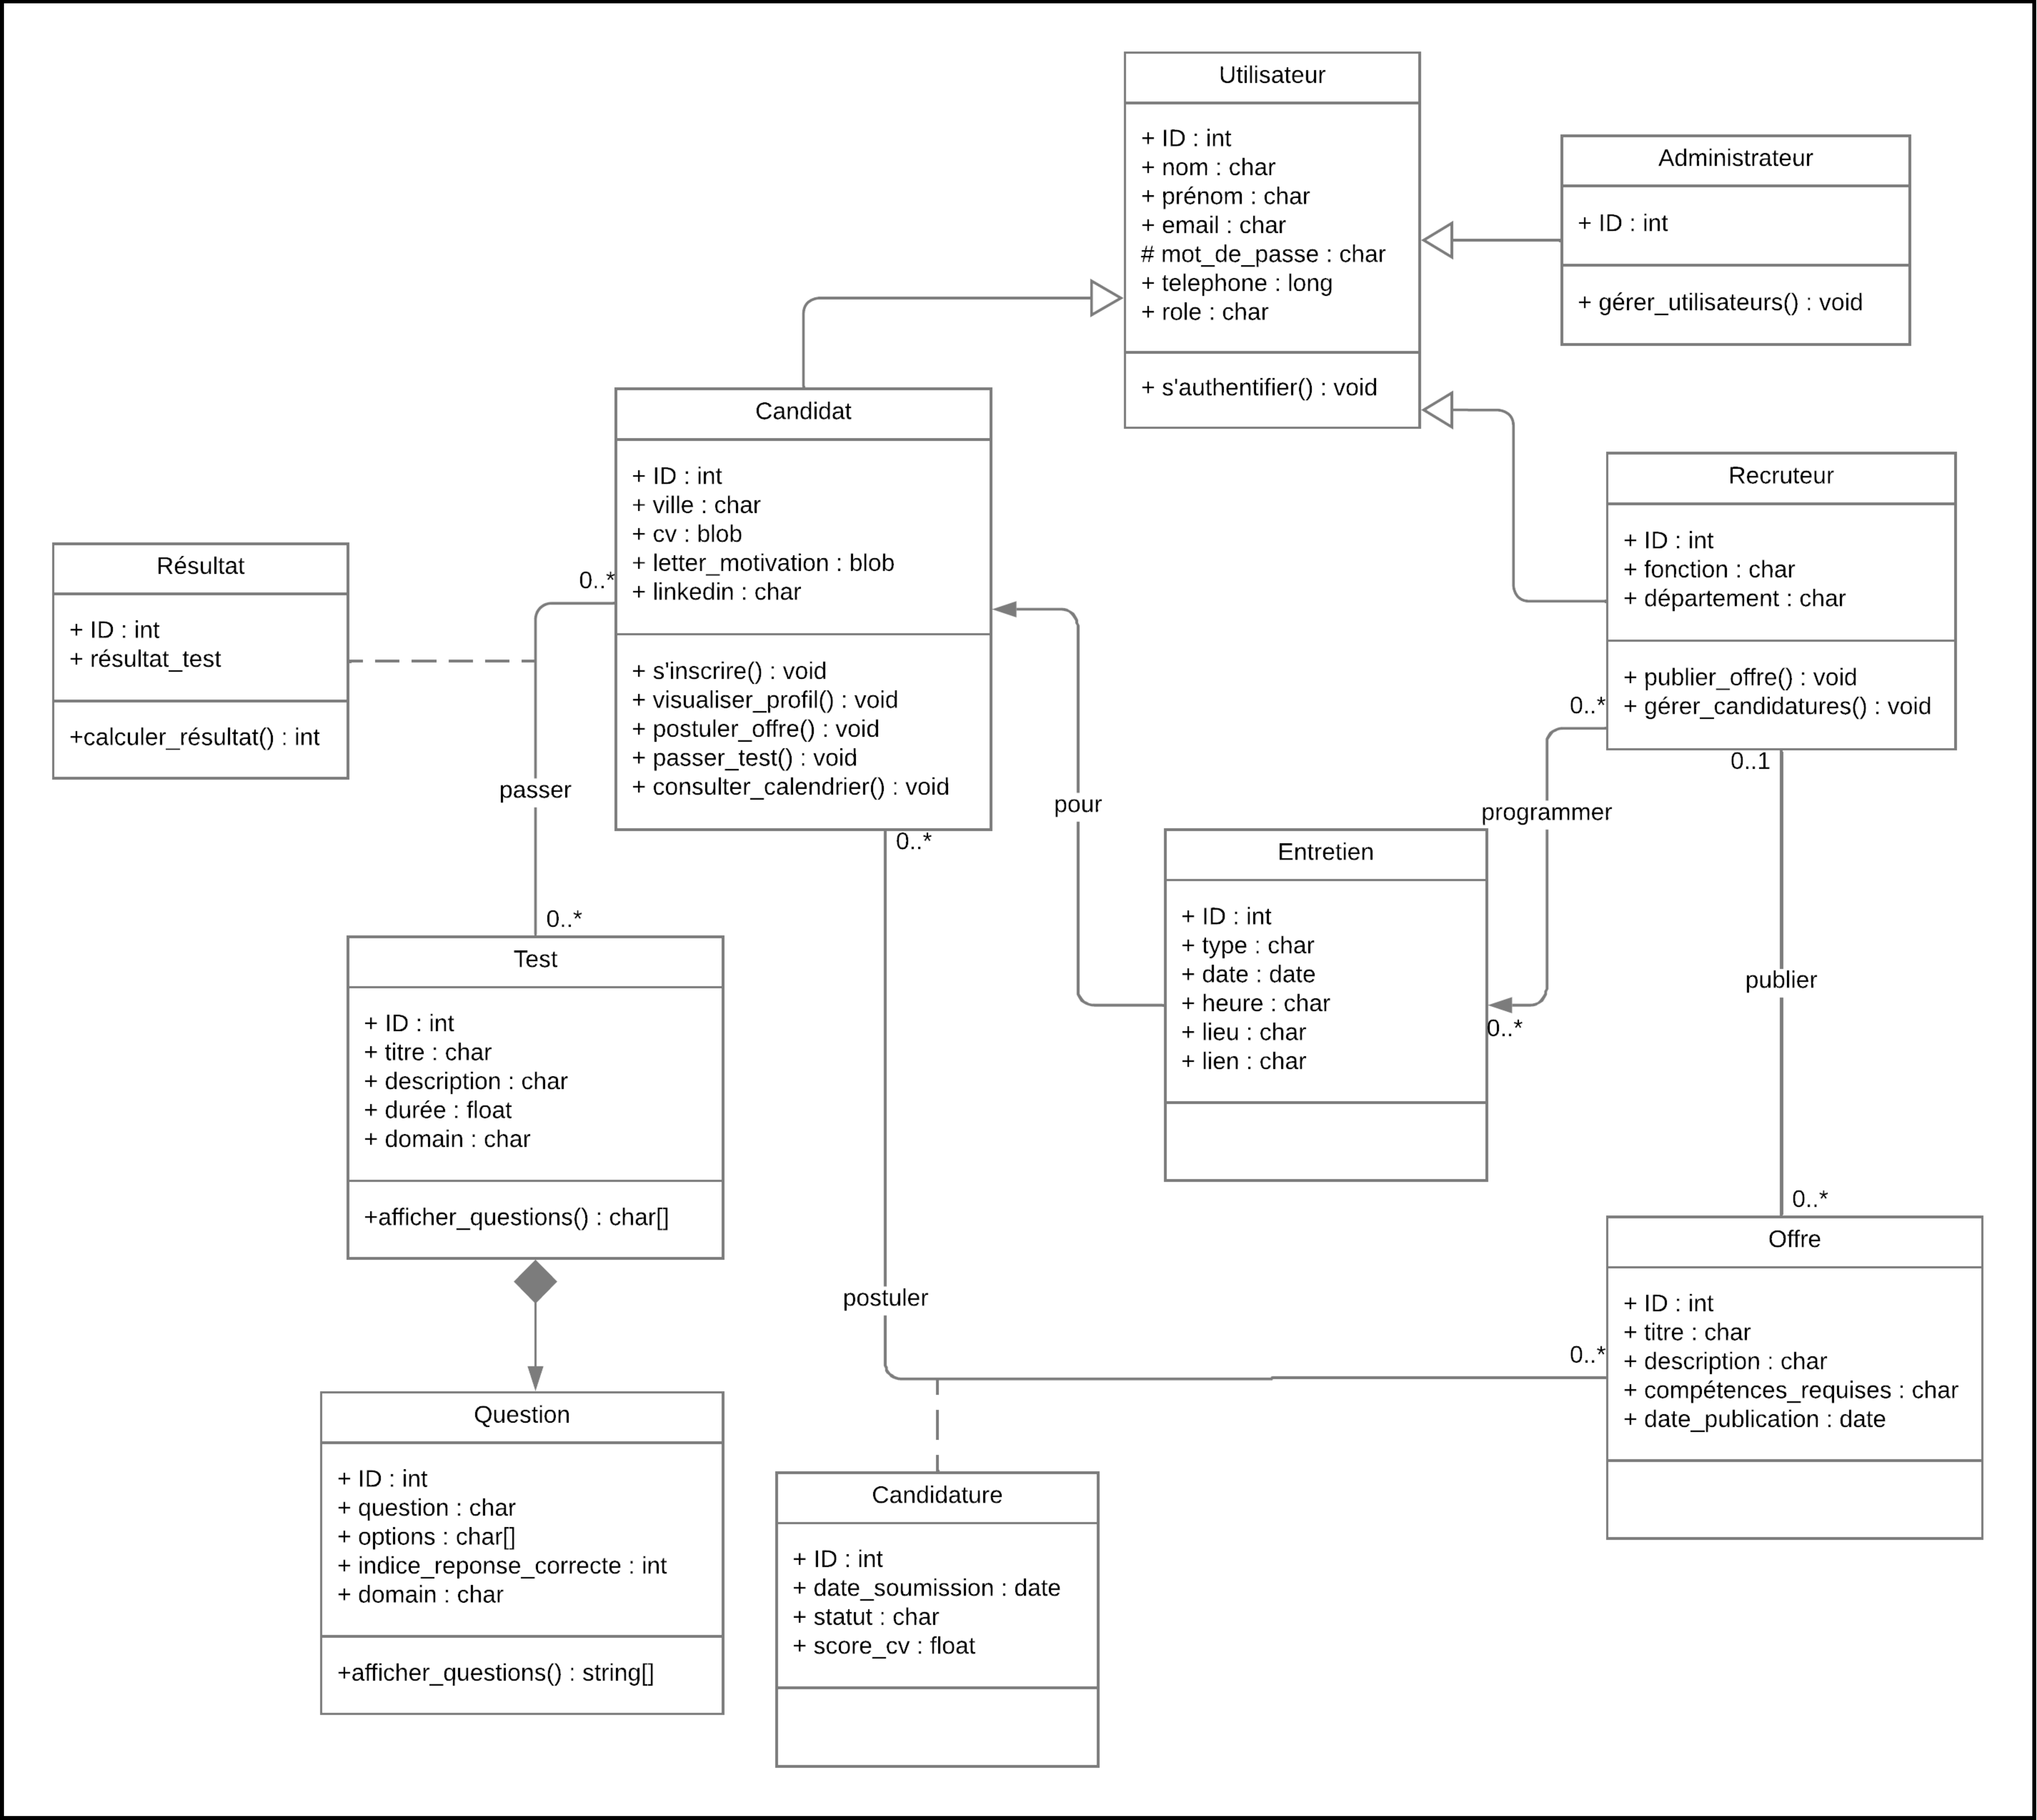
\includegraphics[scale=0.3]{Images/classDiagram.png} % Replace with the actual filename of the IBM logo image
   \caption{Diagramme de classes}
   \label{fig:ClassDiag}
\end{figure}
%commentaire !!!!



\section{Diagrammes de séquence}
Le diagramme de séquence offre une représentation claire 
et détaillée des interactions entre les divers objets ou 
composants d’un système. Dans le cadre de notre projet, 
ce diagramme nous permet de modéliser de manière précise et 
compréhensible les échanges entre les utilisateurs et l’interface 
utilisateur de l’application, ainsi que les interactions entre cette 
dernière, le serveur et la base de données associée.

\begin{figure}[htbp]
   \centering
   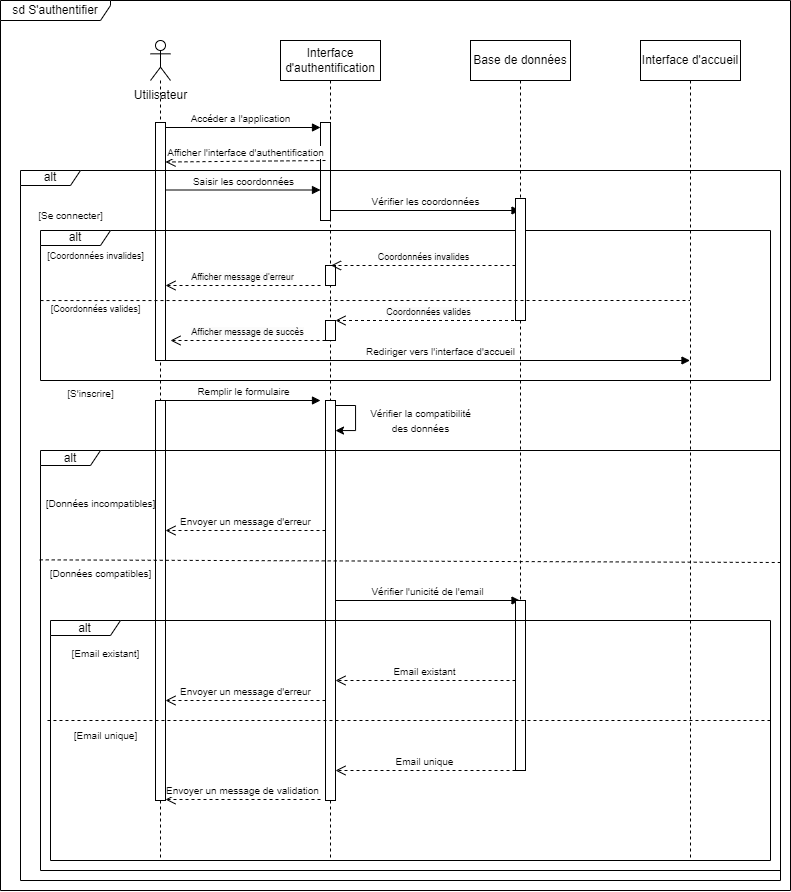
\includegraphics[scale=0.8]{Images/auth.png} % Replace with the actual filename of the IBM logo image
   \caption{Diagramme de séquence d’authentification}
   \label{fig:seq1}
\end{figure}

\begin{figure}[htbp]
   \centering
   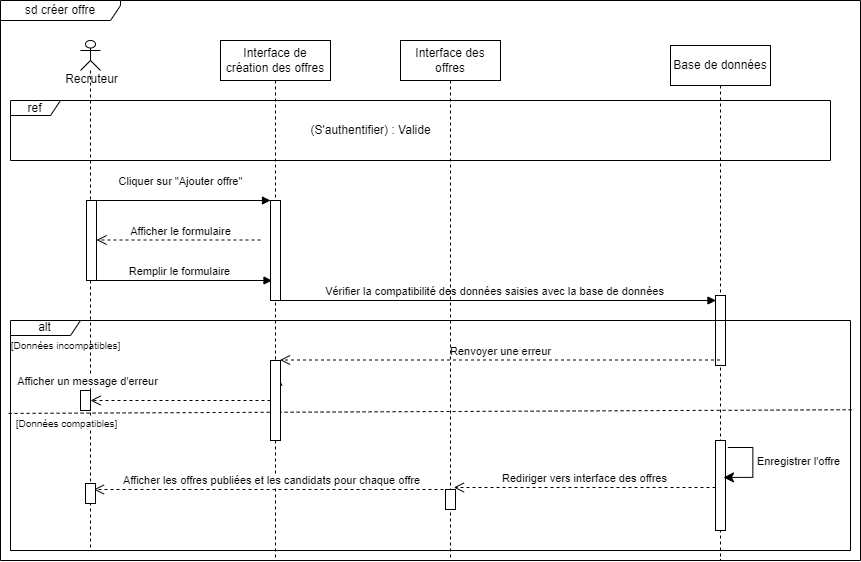
\includegraphics[scale=0.8]{Images/creerOffre.png} % Replace with the actual filename of the IBM logo image
   \caption{Diagramme de séquence de création des offres}
   \label{fig:seq2}
\end{figure}

\begin{figure}[htbp]
   \centering
   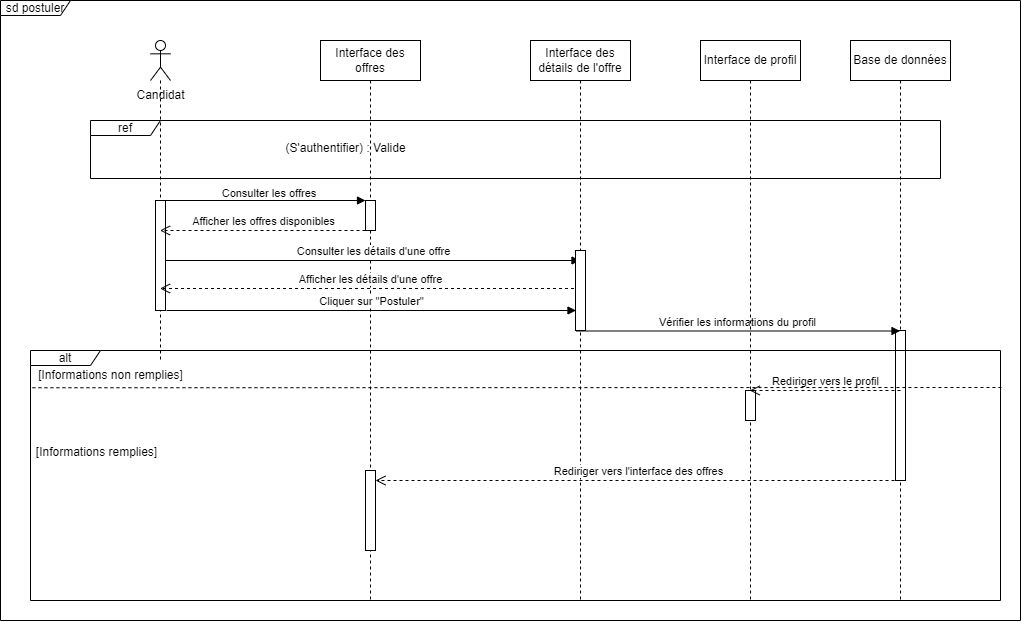
\includegraphics[scale=0.6]{Images/postuler.png} % Replace with the actual filename of the IBM logo image
   \caption{Diagramme de séquence de postulation}
   \label{fig:seq3}
\end{figure}

\begin{figure}[htbp]
   \centering
   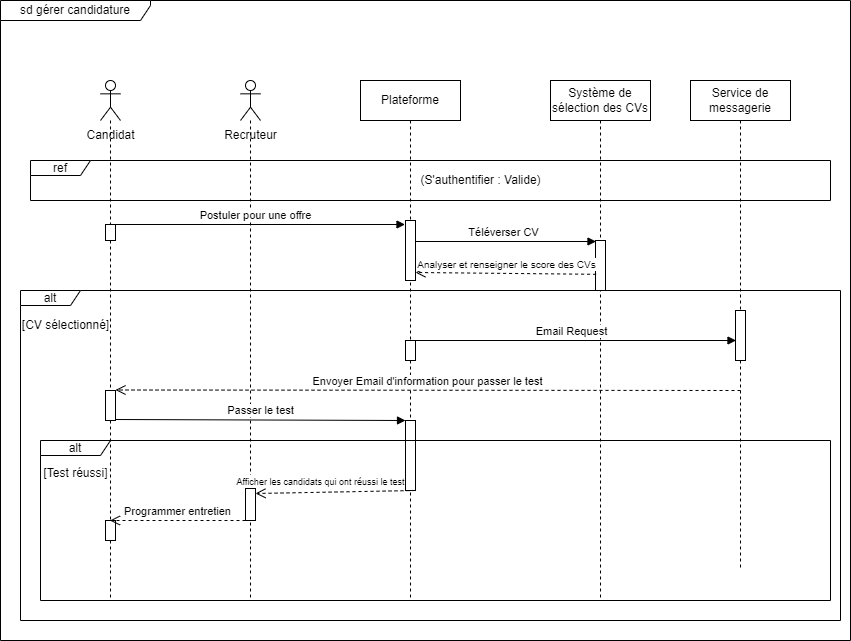
\includegraphics[scale=0.8]{Images/gererCandidature.png} % Replace with the actual filename of the IBM logo image
   \caption{ Diagramme de séquence de gestion des candidatures}
   \label{fig:seq4}
\end{figure}


\section{Conclusion}
Ce chapitre a présenté une conception détaillée 
de la solution, en se focalisant sur l'architecture 
technique et les différents éléments nécessaires 
pour une mise en œuvre efficace. Nous avons d'abord 
élaboré les maquettes UX/UI pour aligner les attentes 
des utilisateurs finaux avec les fonctionnalités 
du système, puis nous avons décrit l'architecture 
physique en détaillant les serveurs et les couches 
réseau impliquées. Ensuite, l'architecture logique 
a été illustrée, mettant en avant l'utilisation de 
4D Server et ORDA pour simplifier le développement. 
Enfin, nous avons détaillé les diagrammes de classes et de séquence, fournissant une vue précise des interactions dynamiques et de la structure du système, garantissant ainsi une conception robuste, modulable et évolutive.
% % Define the page style
\fancypagestyle{chapterstyle}{
   \fancyhead[L]{\nouppercase{\rightmark}}
   \fancyhead[R]{Projet de fin d'études 2023-2024}
   \fancyfoot[C]{\vspace{20pt}\thepage} % Adjust the vertical space here
   \setlength{\headheight}{20pt}
   \setlength{\footskip}{30pt} % Adjust the value as needed
}





\chapter{Implémentation et validation}
\pagestyle{chapterstyle}


\newpage
\vspace{1cm}

\section{Introduction}
%  Cette phase 
% consiste à concrétiser le modèle conceptuel précédemment établi 
% en composants logiciels formant notre système, puis à vérifier 
% leur bon fonctionnement. Dans ce chapitre, nous allons présenter 
% de manière succincte les différents outils que nous avons utilisés 
% tout au long du développement et de la validation de notre 
% application.
Dans ce chapitre, nous présentons de manière concise les différents 
outils et technologies utilisés tout au long du développement et de la validation de notre 
application, accompagnés des captures d'écran illustrant leur mise en œuvre.



\section{Outils et technologies de développement}
\subsection{Outils de conception}

\large 
\textbf{Figma}

\begin{figure}[htbp]
   \centering
   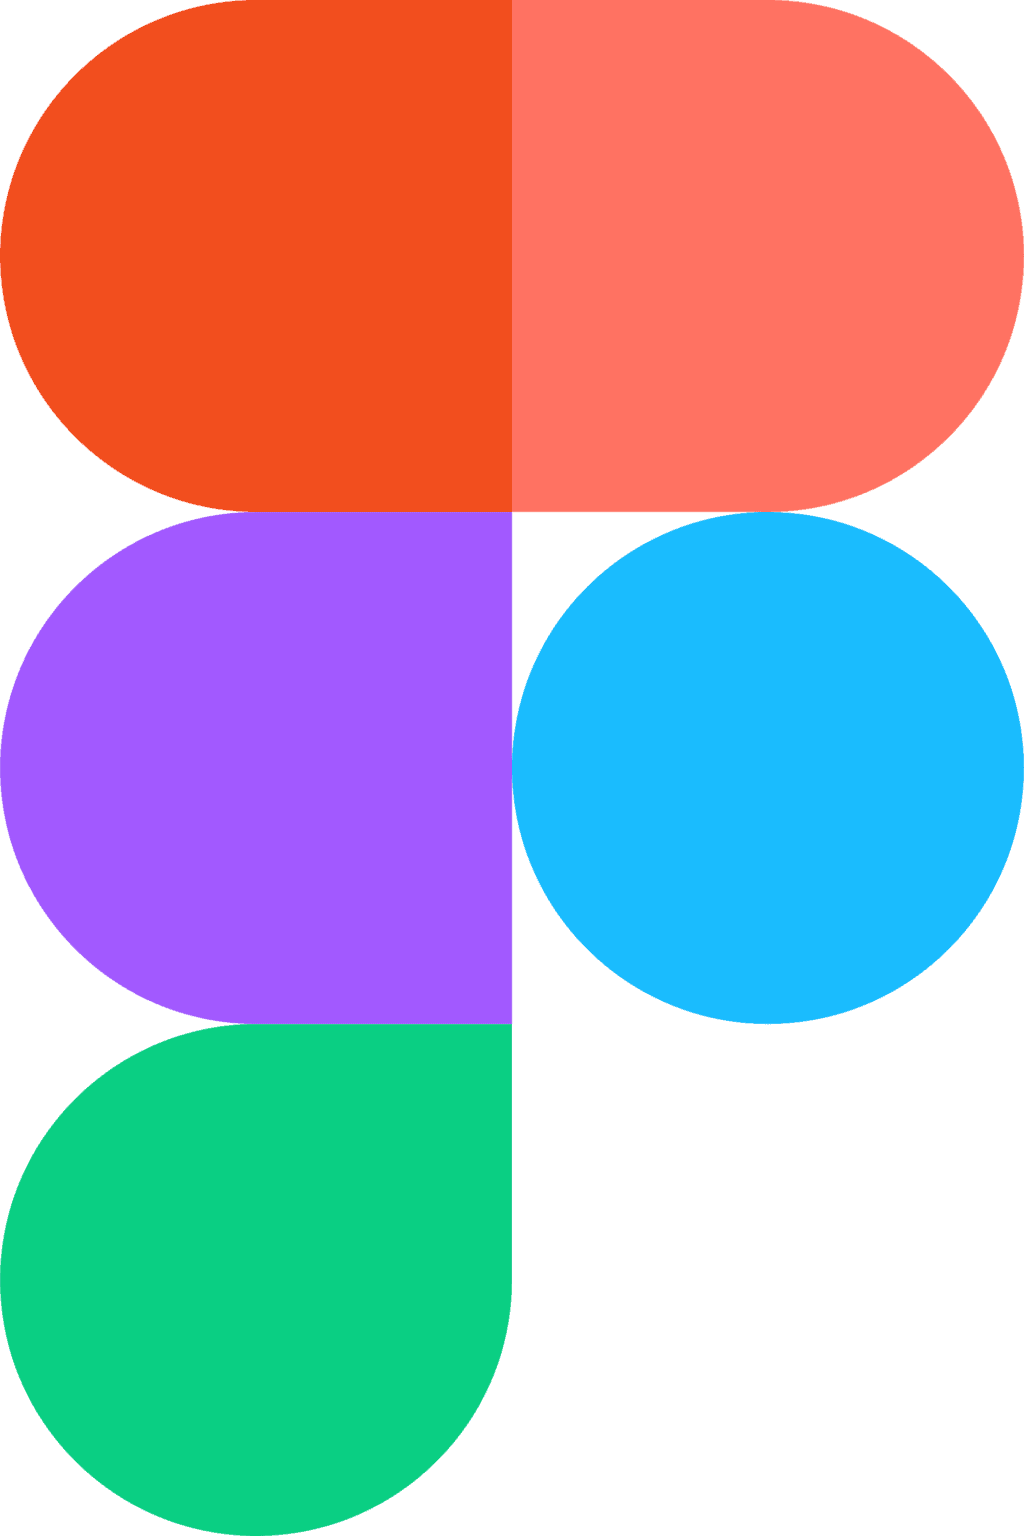
\includegraphics[scale=0.03]{Images/figma.png} 
   \caption{Logo Figma\cite{figma}}
   \label{fig:figma}
\end{figure}
Figma est un outil de design collaboratif en ligne pour la 
création d'interfaces utilisateur. Il permet de créer des 
maquettes et des prototypes interactifs, facilitant la 
collaboration en temps réel\cite{figma}. C'est l'outil que nous avons utilisé 
pour créer les maquettes de notre projet.
\newline

\large 
\textbf{Lucidchart}
\begin{figure}[htbp]
   \centering
   
\includegraphics[scale=0.2]{Images/lucid.jpeg} 
   \caption{Logo Lucidchart\cite{LucidChart}}
   \label{fig:lucid}
\end{figure}

Lucidchart est un outil en ligne pour créer et partager des 
diagrammes et des visualisations de données. Il permet de 
dessiner des diagrammes de flux, des organigrammes, des cartes 
conceptuelles, et bien d'autres schémas \cite{LucidChart}. Cet outil a été utilisé pour
la conception des différents diagrammes de cas d'utilisation, de classe et de séquence.

\subsection{Environnement de développement}
\large 
\textbf{Visual Studio Code}

\begin{figure}[htbp]
   \centering
   
\includegraphics[scale=0.06]{Images/vs.png} 
   \caption{Logo Visual Stduio Code\cite{vsCode}}
   \label{fig:vscode}
\end{figure}

Visual Studio Code est un éditeur de texte open source,
 gratuit et multiplateforme (Windows, Mac et Linux), 
 développé par Microsoft\cite{vsCode}. Cet environnement de développement 
 a été utilisé pour développer la partie frontend du projet, gérer la console Git et rédiger le rapport en utilisant l'extension LaTeX Workshop.
\newline

\large 
\textbf{4D Client}

\begin{figure}[htbp]
   \centering
   
\includegraphics[scale=0.2]{Images/4dcl.png} 
   \caption{Logo 4D Client\cite{4d}}
   \label{fig:4dcl}
\end{figure}

4D vous permet de construire des applications client-serveur 
personnalisées qui sont homogènes, multiplateformes et avec 
une option de mise à jour automatique. Les applications 
client et serveur sont configurées dans la page Client/Serveur 
de la boîte de dialogue Construire une application \cite{4d}.
Cet outil nous a servi pour developpe la partie backend du projet 
en se concentrant sur le volet metier du projet, il facilite la gestion
des données et la mise en place de la base de données graphique.
\newline

\large 
\textbf{4D Serveur}

\begin{figure}[htbp]
   \centering
   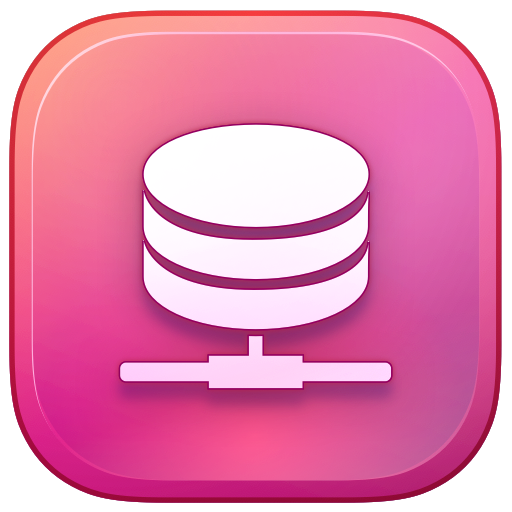
\includegraphics[scale=0.2]{Images/4dsrv.png} 
   \caption{Logo 4D Serveur\cite{4d}}
   \label{fig:4dsrv}
\end{figure}

4D Server est un composant logiciel de la plateforme de développement 
4D qui permet le déploiement et la gestion
d’applications client-sebrveur. Il offre un environnement robuste 
et évolutif pour héberger des applications 4D, 
permettant à plusieurs utilisateurs d’y accéder et d’interagir avec
l’application simultanément. 4D Server agit comme un hub centralisé, 
gérant le stockage des données, le traitement et la communication entre 
le serveur et les applications clientes connectées. Il prend en charge 
des fonctionnalités telles que l’accès simultané aux données partagées, 
la gestion des transactions, les contrôles de sécurité et la collaboration
multi-utilisateur\cite{4d}.
\newline

Ces caractéristiques du serveur 4D permettent de garantir les exigences non fonctionnelles mentionnées précédemment : la disponibilité, la performance et l'évolutivité. 
\newline

\large 
\textbf{Postman}

\begin{figure}[htbp]
   \centering
   
\includegraphics[scale=0.4]{Images/postman.png} 
   \caption{Logo postman\cite{Postman}}
   \label{fig:postman}
\end{figure}

Postman fournit une interface conviviale où les développeurs 
peuvent spécifier les paramètres de requête, les entêtes, 
les corps de requête, les méthodes HTTP, etc. Ils peuvent 
également inspecter les réponses des serveurs, valider les 
résultats et effectuer des tests automatisés pour s’assurer que 
l’API fonctionne correctement\cite{Postman}. Le rôle de Postman 
dans notre projet est indispensable, car il permet de vérifier 
le bon fonctionnement de la partie backend et de valider les 
données envoyées et reçues entre le serveur et le client.
\newline

\large 
\textbf{GitLab}

\begin{figure}[htbp]
   \centering
   
\includegraphics[scale=0.6]{Images/gitlab.jpg} 
   \caption{Logo GitLab\cite{gitlab}}
   \label{fig:gitlab}
\end{figure}
GitLab est une plateforme DevOps complète proposée sous la forme 
d’une application unique. Elle révolutionne le développement, 
la sécurité, l’exploitation et la collaboration entre les équipes. 
Créez, testez et déployez des logiciels plus rapidement en 
n’utilisant qu’une seule solution. GitLab nous a permis de collaborer tout au long du projet pour gérer les versions, les modifications et les mises à jour du code.
\subsection{Langages de développement}
\large 
\textbf{4D}

\begin{figure}[htbp]
   \centering
   
\includegraphics[scale=0.8]{Images/logo-4d.jpg} 
   \caption{Logo 4D\cite{4d}}
   \label{fig:4D}
\end{figure}
Le langage 4D est un langage de programmation spécifique à la
plateforme utilisé dans l’environnement de développement 4D pour
créer des applications professionnelles et des bases de données. 
Il est conçu pour simplifier le développement d’applications 
en fournissant des fonctionnalités spécifiques à la gestion des 
données et des interfaces utilisateur\cite{4d}. 
\newline

Nous avons utilisé le langage 4D principalement pour l'insertion de données de type objet. Ce langage nous a également permis de créer des méthodes et des classes selon les besoins du projet. Grâce à ses capacités avancées de manipulation des objets, 4D a facilité la structuration et la gestion des données complexes. En outre, la possibilité de définir des méthodes et des classes a offert une grande flexibilité dans l'implémentation de la logique métier, rendant le développement plus modulable et maintenable.
\newline

\large 
\textbf{TypeScript}
\begin{figure}[h]
   \centering
   
\includegraphics[scale=0.05]{Images/ts.png} 
   \caption{Logo TypeScript\cite{TypeScript}}
   \label{fig:ts}
\end{figure}

TypeScript, développé par Microsoft, est un surensemble de 
JavaScript qui ajoute des types statiques, permettant de
détecter les erreurs dès la phase de développement. Il compile 
en JavaScript standard et est compatible avec tous les 
navigateurs. TypeScript offre des fonctionnalités avancées 
comme les interfaces, les énumérations et les génériques, 
et bénéficie d'un excellent support des outils de développement, 
facilitant l'auto-complétion et la refactorisation\cite{TypeScript}. 
Ces caractéristiques en 
font un choix idéal pour les applications à grande échelle 
où la qualité et la maintenabilité du code sont cruciales, 
ce qui nous a conduit à l'adopter pour notre projet évolutif.
\newline

\large
\textbf{HTML}
\begin{figure}[htbp]
   \centering
   
\includegraphics[scale=0.15]{Images/html.png} 
   \caption{Logo HTML\cite{HTML}}
   \label{fig:html}
\end{figure}

HTML est un langage de balisage conçu pour représenter les pages
 web. C’est un langage permettant d’écrire de l’hypertexte, 
 d’où son nom. HTML permet également de structurer sémantiquement 
 et logiquement et de mettre en forme le contenu des pages, 
 d’inclure des ressources multimédias dont des images, des 
 formulaires de saisie et des programmes informatiques\cite{HTML}.
\newline

\subsection{Frameworks}
\large
\textbf{React}
\begin{figure}[htbp]
   \centering
   \includegraphics[scale=0.1]{Images/react.png} 
   \caption{Logo React\cite{React}}
   \label{fig:react}
\end{figure}

React est une bibliothèque JavaScript frontale open source 
permettant de créer des interfaces utilisateur ou des composants 
d'interface utilisateur. Il est maintenu par Facebook et une 
communauté de développeurs individuels et d'entreprises. 
React peut être utilisé comme base dans le développement 
d'applications monopages ou mobiles. Nous avons choisi 
d'utiliser ce framework dans notre projet en raison de sa 
capacité à créer des interfaces utilisateur dynamiques et 
réactives, de sa gestion efficace de l'état et des mises à 
jour en temps réel, ainsi que de la réutilisabilité de ses 
composants\cite{React}. Ces caractéristiques facilitent la maintenance, 
la scalabilité et l'évolution de notre application, 
répondant ainsi aux besoins de notre projet.
\newline

\large
\textbf{Tailwind}
\begin{figure}[htbp]
   \centering
   \includegraphics[scale=0.5]{Images/tailwind.png} 
   \caption{Logo Tailwind\cite{Tailwind}}
   \label{fig:tailwind}
\end{figure}

Tailwind est un framework CSS qui fournit un catalogue complet 
de classes et d’outils CSS permettant de styliser facilement un 
site web ou une application. Nous avons choisi d'utiliser 
Tailwind dans notre projet en raison de plusieurs avantages 
clés. Premièrement, Tailwind facilite une conception rapide et 
efficace grâce à ses classes utilitaires préconçues, éliminant 
le besoin d'écrire des CSS personnalisés pour chaque élément. 
Deuxièmement, il offre une grande flexibilité et permet de créer 
des designs réactifs et cohérents. Enfin, Tailwind améliore 
la maintenabilité du code en gardant les styles directement dans 
les classes HTML, ce qui simplifie la gestion des styles et 
réduit les conflits CSS\cite{Tailwind}. Ces caractéristiques nous ont permis de 
développer une interface utilisateur esthétique et fonctionnelle 
tout en accélérant le processus de développement.
\newline

\large
\textbf{Axios}
\begin{figure}[h]
   \centering
   \includegraphics[scale=0.5]{Images/axios.png}
   \caption{Logo Axios\cite{Axios}}
\end{figure}

Dans le contexte de notre projet, nous avons intégré Axios en 
raison de sa capacité à simplifier la gestion des requêtes HTTP 
entre notre frontend basé sur React et notre backend. Axios nous 
permet de réaliser des appels API de manière efficace et fiable, 
en utilisant une syntaxe claire et intuitive. Cela facilite 
l'intégration des fonctionnalités d'interaction avec le serveur, 
comme la récupération et l'envoi de données dynamiques, 
essentielles pour assurer la réactivité et la performance de 
notre application. En utilisant Axios avec React, nous avons 
pu maintenir un flux de données fluide et sécurisé, répondant 
ainsi aux exigences de notre projet en termes de communication 
client-serveur.
\newline

\large
\textbf{Cypress}
\begin{figure}[htbp]
   \centering
   \includegraphics[scale=0.6]{Images/cy.jpg} 
   \caption{Logo Cypress\cite{Cypress}}
   \label{fig:cypress}
\end{figure}

Cypress est un framework de tests bout-en-bout open source qui 
s'intègre parfaitement avec notre pile technologique, notamment 
React et Tailwind CSS. Nous l'avons utilisé pour garantir le bon 
fonctionnement et la bonne stylisation de nos composants 
frontaux. Cypress facilite l'écriture et la maintenance des 
tests grâce à son support pour JavaScript moderne et son 
exécution directe dans le navigateur. Ses outils de débogage 
et de visualisation des tests nous permettent de résoudre 
rapidement les problèmes\cite{Cypress}. En automatisant nos tests avec Cypress, 
nous avons assuré une couverture complète des fonctionnalités 
critiques et une détection précoce des régressions, maintenant 
ainsi la qualité de notre code.

% travail realise
\section{Captures d'écran}
Cette section présente des captures d'écran de diverses interfaces de notre application, 
accompagnées de descriptions  détaillées.  Chaque  capture  illustre une interface 
spécifique de l'application et met en avant les fonctionnalités principales disponibles. 
% Les descriptions fournissent des informations sur la disposition de l'interface, 
% les boutons et les menus pertinents, ainsi que sur les actions que les utilisateurs 
% peuvent réaliser.
\subsection{Page d'accueil}

La page  d’accueil est  conçue pour offrir une expérience utilisateur intuitive et 
informative. En haut une  barre  de navigation avec le logo de l’application et 
des liens vers les principales sections comme le bouton “sign in” qui permet l’utilisateur de  
naviguer vers la page d’authentification. La section principale attire immédiatement 
l’attention avec un message accrocheur et une illustration attrayante, présentant 
l'objectif de la  plateforme. Les catégories d’emploi sont mises en  avant. 
Une section de guide des utilisateurs à travers des étapes simples de candidature. 
Un appel à l’action “Ready to start ?”  encourage l'engagement, en  redirigeant 
l’utilisateur vers la page d’inscription.  
\begin{figure}[htbp]
   \centering
   \includegraphics[scale=0.7]{screens/accueil2.jpg} 
   \caption{Page d'accueil}
   \label{fig:accueil}
\end{figure}

\vspace{2cm}
\subsection{Authentification}
En cliquant le bouton “Sign In”, l’utilisateur sera redirigé vers la page d’authentification. 
Les utilisateurs peuvent saisir leurs  informations  d’identification, 
leur email et leur mot de passe, dans les champs correspondants. 
 Si les données saisies sont 
valides, l’utilisateur va accéder à son espace personnel, en fonction de 
son rôle.
\newline
\begin{figure}[htbp]
   \centering
   \includegraphics[scale=0.5]{screens/signin.jpg} 
   \caption{Page d'authentification}
   \label{fig:accueil}
\end{figure}

Si les informations sont incorrectes, un message d’erreur "Wrong Email or Password" 
sera affiché. Si l’utilisateur oublie son mot de passe, il peut le réinitialiser en 
cliquant sur la fonctionnalité "Forgot Password  ?",  qui  le redirigera vers une autre 
page illustrée par la figure \ref{fig:forgotPass}. Sur cette page, il pourra remplir 
son  email. Une  fois soumis, l'application vérifiera immédiatement la présence de 
l'adresse email dans sa base de données. Si elle n'est pas trouvée, un message d’erreur 
sera affiché. 
\newline
\begin{figure}[htbp]
   \centering
   \includegraphics[scale=0.6]{screens/forgot.jpg} 
   \caption{Mot de passe oublié}
   \label{fig:forgotPass}
\end{figure}
\vspace{5cm}

% Sinon, si  l'email est  trouvé, un  courriel sera envoyé à l'adresse fournie via la 
% méthode POST, contenant le  nouveau mot de  passe, comme illustré dans la figure.
Sinon, si l'adresse mail est trouvée, l'utilisateur recevra
un email de réinitialisation de mot de passe dans sa boite mail, comme illustré dans la figure \ref{fig:mailPass}.

\begin{figure}[htbp]
   \centering
   \includegraphics[scale=0.26]{screens/mailForgot.png} 
   \caption{Exemple d'un email pour réintialiser le mot de passe}
   \label{fig:mailPass}
\end{figure}

\subsection{Espace Candidat}
\subsubsection{La page d’inscription}
Le candidat peut accéder au formulaire d’inscription à partir du bouton 
“Ready to start?” ou le bouton “Sign up” de la page d’authentification. 
Ce forumulaire comme il est représenté sur la figure \ref{fig:singup}. 
À droite, la section pour l'inscription comporte des champs de 
formulaire pour entrer des informations personnelles, 
y compris le prénom, le nom, le courriel, le mot de  passe, et  
le numéro de téléphone. En bas, un bouton "REGISTER” permet de finaliser 
l'inscription. Juste en dessous, il y a un lien "Already have an account ? Sign In" 
pour rediriger les utilisateurs vers la page de connexion s’ils ont déjà 
un compte.

\begin{figure}[htbp]
   \centering
   \includegraphics[scale=0.4]{screens/signup.jpg} 
   \caption{Page d'inscription}
   \label{fig:singup}
\end{figure}

\subsubsection{Profil}
Après l'authentification, chaque utilisateur se voit attribuer 
un  rôle (candidat, recruteur ou administrateur),  qui  
détermine  l'accès  à son  espace dédié. Prenons d'abord le cas 
où l'utilisateur est un candidat : il est redirigé directement 
vers son profil, comme illustré dans la figure \ref{fig:profile}.
\newline

Dans la première section de son profil, le  candidat peut mettre 
à jour sa photo et ses informations personnelles. Dans la 
deuxième section, il  peut ajouter ou mettre à jour son CV et 
sa lettre  de  motivation.  Enfin,  dans  la  dernière section, 
il a la possibilité de réinitialiser son mot de passe pour la 
plateforme.
\newline


\begin{figure}[htbp]
   \centering
   \includegraphics[scale=0.3]{screens/profill.png} 
   \caption{Profil}
   \label{fig:profile}
\end{figure}

\vspace{6cm}

\subsubsection{Postuler à une offre}
En naviguant via le menu de gauche, un simple clic sur le 
bouton "Offres" conduit à la page représentée par la figure \ref{fig:listOffers}.  
Cette  page  présente plusieurs cartes, chacune décrivant une  
offre d'emploi active, et  publiée par un 
recruteur. Chaque carte comprend les détails suivants : 
le titre du poste, la localisation, une description 
du poste, le  type de  contrat (stage, emploi, etc.), et 
le mode de travail (présentiel, télétravail, ou hybride). En haut 
de la page, un menu permet de filtrer les offres d'emploi par 
domaine, tel que DevOps, Data science, et software engineering.
\newline

Chaque page affiche jusqu'à 6 cartes,  avec  une  fonction  de  pagination pour accéder aux offres suivantes.
\begin{figure}[htbp]
   \centering
   \includegraphics[scale=0.2]{screens/cartes.png} 
   \caption{Liste des offres}
   \label{fig:listOffers}
\end{figure}

Comme illustré dans la figure \ref{fig:detailsOffre}, chaque 
carte est dotée de deux boutons. Le premier, intitulé "More", 
permet au candidat d'accéder à une page détaillant l'offre. 
Le deuxième est pour enregistrer l'offre afin de lui accéder par la suite.
Sur cette page, sont présentés aussi le  titre  de  l'offre,  
sa  localisation,  son mode de travail, le type de contrat, 
la description du  poste,  ainsi  que  les exigences 
spécifiques du poste.
\newline
\begin{figure}[htb]
   \centering
   \includegraphics[scale=0.2]{screens/consultOffer.png} 
   \caption{Consulter le detail d'une offre}
   \label{fig:detailsOffre}
\end{figure}
\vspace{3cm}

Si le candidat souhaite postuler à l'offre, il peut cliquer 
sur le  bouton "APPLY NOW". Cela affichera une boîte de 
dialogue confirmant la candidature à l'offre, comme illustré
dans la figure \ref{fig:detailsOffre}.
\newline

\begin{figure}[htbp]
   \centering
   \includegraphics[scale=0.2]{screens/confirmJob2.png} 
   \caption{Confirmation de candidature}
   \label{fig:listOffers}
\end{figure}


En postulant à l'offre choisie, un calcul de score de CV s'effectue. 
Si le score du CV dépasse le seuil défini, le candidat devient éligible à passer 
le test et reçoit un email d'invitation illustré dans la figure \ref{fig:inviteTest}. Dans le cas contraire, le candidat n'est 
pas éligible au test.
\vspace{5cm}
\begin{figure}[htbp]
   \centering
   \includegraphics[scale=0.25]{screens/testInvitation.png} 
   \caption{Exemple d'une invitation au test}
   \label{fig:inviteTest}
\end{figure}

\subsubsection{Mes offres}
En cliquant sur le bouton "My offers" situé dans 
le  menu de  gauche, le candidat peut visualiser ses candidatures et les offres qu'il a enregistré. \\
Les offres enregistrés sont disposées sous forme de cartes dans l'onglet "Saved" comme indiqué dans la figure \ref{fig:saved}.
\\

\begin{figure}[htbp]
   \centering
   \includegraphics[scale=0.2]{screens/saved.png} 
   \caption{Offres enregistrés}
   \label{fig:saved}
\end{figure}

Pour la partie d'historique de candidatures, les  offres auxquelles le  candidat a 
postulé sont affichées dans un tableau en accédant à l'onglet "Applied". Le tableau inclut les éléments suivants: le titre du poste, la date de  
soumission à l'offre, le  lieu, le  statut de la candidature ainsi qu'un bouton "Start test".  
\vspace{3cm}
\begin{figure}[htbp]
   \centering
   \includegraphics[scale=0.2]{screens/myofffers.png} 
   \caption{Historique de candidatures}
   \label{fig:candidatures}
\end{figure}




\subsubsection{Passer le test}
% Après avoir valider la phase du séléction par cv, le candidat doit passer un test lié à sa candidature.
%  Le test consiste en une série de questions à choix multiples.
%  Ces questions sont générées aléatoirement à partir d'un backlog contenant plusieurs questions en fonction du domaine de l'offre.
%  Cette approche garantit la fiabilité et l'équité des tests  entre les candidats.
%  Les tests ont des limites de temps et un candidat a le droit de passer le test lié à une candidature qu'une seule fois

Après avoir validé la phase de sélection par CV, le candidat doit passer un test. Ce test consiste 
en 
une série de questions à choix multiples générées aléatoirement à partir d'un backlog 
contenant plusieurs questions, adaptées au domaine de l'offre. Cette approche garantit 
une sorte de fiabilité et équité des tests entre les candidats. De plus, chaque test 
a une limite de temps et le candidat n'a droit qu'à une seule tentative par candidature.
\begin{figure}[htbp]
   \centering
   \includegraphics[scale=0.2]{screens/test.png} 
   \caption{Page de test}
   \label{fig:listOffers}
\end{figure}


Si le candidat réussit encore son test, il sera convoqué via email pour passer un entretien avec le recruteur 
chargé de l'offre. Voici un exemple de mail reçu par le candidat représenté dans la figure \ref{fig:mailEntretien}
\vspace{3cm}
\begin{figure}[htbp]
   \centering
   \includegraphics[scale=0.2]{Images/interviewMail.png} 
   \caption{Exemple de convocation à l'entretien}
   \label{fig:mailEntretien}
\end{figure}

\subsubsection{Consulter le calendrier}

Le candidat pourra consulter le calendrier où il trouvera lùense,ble des entretiens qu'il doit passer, comme indiqué dans la figure \ref{fig:calendrierCandid}. 
% Le candidat pourra consulter la page calendrier pour vérifier la 
% date et l'heure de son entretien. Grâce à cette fonctionnalité, les candidats peuvent facilement accéder aux détails de leur rendez-vous, ce qui leur permet de s'organiser efficacement et de se préparer en conséquence pour leur entretien avec le recruteur.
\begin{figure}[htbp]
   \centering
   \includegraphics[scale=0.18]{screens/calendarCand.png} 
   \caption{Page de calendrier}
   \label{fig:calendrierCandid}
\end{figure}


% En cliquant sur le titre d'un entretien, il accédera à un dialogue contenant plus de détails tels que la date, l'heure exacte, 
% et l'emplacement de l'entretien. Pour les entretiens présentiel, l'emplacement physique sera précisé, tandis que pour les entretiens en ligne, un lien vers Zoom ou toute autre plateforme similaire sera fourni.
En cliquant sur le titre d'un entretien, le candidat accédera à un dialogue contenant plus de détails, tels que la date, l'heure exacte 
et l'emplacement de l'entretien. Pour les entretiens en présentiel, l'emplacement physique sera précisé, tandis que pour les entretiens en ligne, 
un lien vers Zoom ou toute autre plateforme similaire sera fourni.
% \vspace{2cm}
\begin{figure}[htbp]
   \centering
   \includegraphics[scale=0.3]{screens/detail interview.png} 
   \caption{Détails de l'entretien}
   \label{fig:listOffers}
\end{figure}

% don't forget to uncomment
\subsection{Espace recruteur}
\subsubsection{Page d'accueil du recruteur}
Cette section est dédiée aux recruteurs, qui doivent s'authentifier pour accéder 
directement à leur page d'accueil, illustrée dans la figure\ref{fig:homeRecr}. La première 
partie de cette page présente les statistiques détaillées des offres publiées 
par le recruteur, organisées par localisation et département. 
% Cette visualisation permet de suivre l'évolution des indicateurs de performance 
% des offres, notamment le nombre total d'offres actives, le nombre de candidatures 
% reçues pour chaque poste, et d'autres métriques pertinentes. 

\begin{figure}[htbp]
   \centering
   \includegraphics[scale=0.18]{screens/homeRecr.png} 
   \caption{Page d'accueil du recruteur}
   \label{fig:homeRecr}
\end{figure}

La deuxième partie de cette page d'accueil offre une liste détaillée de toutes 
les offres d'emploi actuellement gérées par le recruteur. Chaque offre est 
présentée avec son titre, sa date de publication et son statut (actif ou clos). 
Pour chaque offre, le recruteur a la possibilité de visualiser les détails 
complets. De plus, un bouton "Add Offer" est 
disponible pour permettre aux recruteurs de créer de nouvelles opportunités 
d'emploi en fonction des besoins évolutifs de l'organisme.

\subsubsection{Publier une offre}

Cette fonctionnalité permet aux recruteurs de créer une nouvelle offre, en saisissant les informations suivantes.
\begin{enumerate}
   \item Job Title (Titre du poste)
   \item Job Location (Lieu de travail)
   \item Work Mode (Mode de travail)
   \item Job Type (Type de contrat)
   \item Required Skills (Compétences requises)
   \item Department (Département)
   \item Domain (Domaine)
   \item Requirements (Exigences)
   \item Job Description (Description du poste)
\end{enumerate}

\begin{figure}[htbp]
   \centering
   \includegraphics[scale=0.15]{screens/addOffer.png} 
   \caption{Publier une offre d'emploi}
   \label{fig:addOfferFields}
\end{figure}

\subsubsection{Gestion de l'offre d'emploi}
Cette page est essentielle pour le recruteur, lui permettant de gérer en détail chaque offre d'emploi publiée. Elle se compose de plusieurs sections :
\begin{figure}[htbp]
   \centering
   \includegraphics[scale=0.17]{screens/detailsOfferRecr.png}
   \caption{Gestion de l'offre d'emploi}
   \label{fig:listOffers}
\end{figure}

\paragraph{- Informations sur l'offre}
Cette section présente les informations essentielles 
relatives à l'offre d'emploi. Le recruteur peut y voir et 
ainsi modifier les détails en cas de changement des besoins. 

\paragraph*{- Modification de l'offre}
Un bouton "Edit Offer" permet au recruteur de mettre 
à jour les informations de l'offre. 
Cela ouvre un formulaire où il peut ajuster les détails 
de l'offre.
\begin{figure}[htbp]
   \centering
   \includegraphics[scale=0.2]{screens/editOffer.png}
   \caption{Modification de l'offre}
   \label{fig
   }
   \end{figure}

\paragraph*{- Liste des candidats}
Cette section permet au recruteur de visualiser et gérer les candidatures pour une offre d'emploi spécifique. 
Chaque entrée de candidature comprend les détails suivants :
\begin{itemize}
   \item[•] Nom du candidat : Le nom complet du candidat
   \item[•] Email : L'adresse email du candidat.
   \item[•] Score du CV : Un score numérique représentant la compatibilité du CV du candidat avec les exigences de l'offre d'emploi.
   \item[•] Résultat du test : Indique si le candidat a réussi le test, et éventuellement, la note obtenue après l'évaluation.
   \item[•] Statut de la candidature : État actuel de la candidature (En cours, Rejetée, Acceptée).
   \item[•] Actions disponibles pour chaque candidature :
      \begin{enumerate}
         \item Voir le CV : Permet aux recruteurs de consulter le CV complet du candidat pour évaluer ses qualifications plus en détail.
         \item Planifier un entretien : Ouvre une interface pour programmer un entretien avec le candidat sélectionné.
         \item Accepter le candidat : Change le statut de la candidature à "Acceptée", indiquant que le candidat a été retenu pour le poste,
         par la suite un mail de confirmation est envoyé au candidat. 
         \newline
         \newline
      \end{enumerate}
\end{itemize}
\vspace{3cm}
\begin{figure}[htbp]
   \centering
   \includegraphics[scale=0.18]{screens/listCandidates.png}
   \caption{Liste des candidats ayant postulé à l'offre}
   \label{fig:candidaturesRec}
\end{figure}

% Voici un exemple de mail envoyé lorsque le recruteur accepte la candidature d'un candidat, figure \ref{fig:}.
% \begin{figure}[htbp]
%    \centering
%    \includegraphics[scale=0.18]{screens/listCandidates.png}
%    \caption{Exemple de mail d'acceptation de candidat}
%    \label{fig:chihaja}
% \end{figure}

\paragraph*{Planifier un entretien}

Après la validation du CV et la réussite du test, le recruteur peut 
planifier un entretien avec le candidat. Cette étape est cruciale pour 
évaluer plus en détail les compétences et l'adéquation du 
candidat avec l'entreprise. 
Le processus est 
réalisé comme suit :

\begin{enumerate}
    \item \textbf{Accès à la planification d'entretien :}
        \begin{itemize}
            \item[•] \textbf{Via l'icône de planification :} En cliquant sur une icône dédiée dans l'interface utilisateur, le recruteur peut accéder à un formulaire de planification d'entretien.
            \item[•] \textbf{Via le menu de gauche :} En naviguant dans le menu de gauche, le recruteur peut accéder directement au calendrier où il peut voir les créneaux disponibles pour planifier l'entretien.
        \end{itemize}
    
    \item \textbf{Sélection du créneau d'entretien :}
        \begin{itemize}
            \item[•] Une fois dans l'interface de planification, le recruteur peut sélectionner un créneau horaire convenable.
            \item[•] Des détails tels que la date, l'heure et l'emplacement de l'entretien peuvent être spécifiés et confirmés dans ce formulaire.
        \end{itemize}
    
    \item \textbf{Confirmation et envoi de l'invitation :}
        \begin{itemize}
            \item[•] Une fois le créneau sélectionné et les détails finalisés, une invitation à l'entretien est envoyé au candidat par email.
            \item[•] L'invitation contient les informations essentielles comme la date, l'heure, l'emplacement physique ou le lien de la réunion en ligne pour l'entretien.
            \\
            \\
            \\
            \\
         \\
         \\
         \end{itemize}
\end{enumerate}

% Exemple d'icône pour la planification d'entretien
\begin{figure}[htbp]
   \centering
   \includegraphics[scale=0.18]{screens/schedule.png} 
   \caption{Planification d'un entretien}
   \label{fig:scheduleIcon}
\end{figure}

\paragraph*{Accepter un candidat}
Une fois que le recruteur a terminé l'entretien avec le candidat,
il pourra accepter le candidat via l'icone de validation dans la figure \ref{fig:candidaturesRec}.
En suite un email est envoyé au candidat pour lui informer de 
l'acceptation de sa candidature, comme illustré dans la figure \ref{fig:mailAccept}.
\begin{figure}[htbp]
   \centering
   \includegraphics[scale=0.2]{screens/acceptCandidate.png}
   \caption{Accepter un candidat}
   \label{fig:mailAccept}
   \end{figure}




\subsection{Espace Administrateur}

\subsubsection{Consulter le tableau de bord}

Le tableau de bord administratif, illustré dans la figure \ref{bordAdmin}, offre un aperçu des statistiques, des graphiques et des listes de candidats et de recruteurs.

\begin{itemize}
    \item[•] \textbf{Statistiques :} affiche les métriques clés telles que le nombre total de candidats, de recruteurs, d'offres d'emploi, etc.
    \item[•] \textbf{Graphiques :} présente une visualisation graphique des données pour une meilleure compréhension des tendances et des performances.
    \item[•] \textbf{Liste des candidats :} montre tous les candidats enregistrés avec leurs informations de contact.
    \item[•] \textbf{Liste des recruteurs :} présente tous les recruteurs avec leurs informations de contact.
\end{itemize}

Au niveau de la table du recruteurs, l'administrateur peut modifier, archiver ou supprimer un recruteur. Ainsi pour le candidat, l'administrateur peut archiver son compte ou le supprimer
\begin{figure}[htbp]
   \centering
   \includegraphics[scale=0.2]{screens/dashAdmin.png} 
   \caption{Le tableau de bord administratif}
   \label{fig:bordAdmin}
\end{figure}



\subsubsection{Ajouter un recruteur}

Cette fonctionnalité permet à l'administrateur d'ajouter de nouveaux recruteurs à l'équipe de gestion des recrutements.
\begin{figure}[htbp]
   \centering
   \includegraphics[scale=0.2]{screens/addRecruiter.png} 
   \caption{Ajouter un recruteur}
   \label{fig:addRec}
\end{figure}




\section{Test et Validation}
% \subsection{Tests unitaires}
% Jest

\subsection{Tests de bout en bout (E2E)}
\subsubsection{Définition et importance}

Dans le contexte de notre projet, le test end-to-end fait référence à une approche de test qui vise à évaluer le système dans son ensemble, en simulant les conditions réelles d’utilisation. Il s’agit d’un type de test qui vérifie le bon fonctionnement du système depuis le début jusqu’à la fin, en testant toutes les étapes intermédiaires et les  interactions entre les  composants. L’importance du test end-to-end dans notre projet réside dans sa capacité  à valider  la fonctionnalité globale du système et à identifier les problèmes d’intégration potentiels. En effectuant des tests end-to-end, vous pouvez vérifier si toutes les parties du système fonctionnent harmonieusement ensemble et satisfont les exigences spécifiées.
\newline

Ces tests permettent également d’évaluer  les  performances  du  système dans des scénarios réalistes, en tenant compte des conditions et des charges de travail typiques. Ils offrent une vision globale de la  qualité  du  système,  en mettant l’accent sur les fonctionnalités essentielles et les  cas  d’utilisation critiques pour les utilisateurs finaux. En résumé, le test end-to-end est essentiel dans votre projet pour s’assurer que toutes les parties du système fonctionnent correctement ensemble, répondent aux exigences et offrent une expérience utilisateur optimale. Il permet d’identifier et de résoudre les problèmes d’intégration pré- cocement, ce qui améliore la  qualité  du  produit  final.  La figure montre le fonctionnement du test E2E par cypress.
\begin{figure}[htbp]
   \centering
   \includegraphics[scale=0.2]{cypress/1.png} 
   \caption{Fonctionnement du test End to End (E2E)}
   \label{fig:listOffers}
\end{figure}



\subsubsection{Exemple sur la page d’authentification}
Pour démarrer, exécutez la commande "npx cypress open" afin d'ouvrir la fenêtre de l'application Cypress sur la figure \ref{fig:cy1}.
\newline

\begin{figure}[htbp]
   \centering
   \includegraphics[scale=0.2]{cypress/2.jpg} 
   \caption{L'ouverture de Cypress}
   \label{fig:cy1}
\end{figure}

Une fois que vous avez ouvert Cypress, sélectionnez l’option de test E2E qui est déjà configurée. Ensuite, on choisit le navigateur sur 
lequel on souhaite exécuter nos tests, comme il est représenté sur la figure \cite{fig:cy2}.
\\
% \\
% \\
% \\
% \\
% \\

\begin{figure}[htbp]
   \centering
   \includegraphics[scale=0.4]{cypress/3.jpg} 
   \caption{Choix de navigateur au niveau de Cypress}
   \label{fig:cy2}
\end{figure}

Une fois le fichier "login.cy.jsx" (spec) créé, vous pouvez procéder à son test sur l'application, comme illustré dans la figure \cite{cy3}.
\\
\\
\\

\begin{figure}[htbp]
   \centering
   \includegraphics[scale=0.4]{cypress/4.jpg} 
   \caption{ End to End test avec Cypress}
   \label{fig:cy3}
\end{figure}

Le résultat du test effectué sur notre page de connexion est sur la figure \cite{cy5}

\begin{figure}[htbp]
   \centering
   \includegraphics[scale=0.4]{cypress/5.jpg} 
   \caption{ Test End to End sur la page de login}
   \label{fig:cy5}
\end{figure}

En résumé, Cypress facilite considérablement les étapes de création, d’exécution et de débogage des tests end-to-end. Il propose une approche conviviale et efficace pour garantir le bon fonctionnement global de notre application en simulant les interactions utilisateur réelles.


\section{Conclusion}
Cette partie du projet a présenté la mise en œuvre de l'application et  la  réalisation  des tests end-to-end. 
Nous avons présenté les différentes étapes de la mise en place de l'application et les différentes
technologies utilisées. Nous avons également présenté les différentes étapes de la réalisation des tests
end-to-end et les différentes technologies utilisées. 
\newline

% \chapter*{Conclusion et Perspectives}
\addcontentsline{toc}{chapter}{Conclusion}


% à compléter..
% perspectives :
% integrer Zoom
% recommendations selon le profile et l historique de candidature
% notifier le candidat si une offre qui match son profile est desormais sur l'application
% permettre au candidat de choisir le créneau preferable pour l entretien
% compatible for all devices 
% integrer des tests plus avancées du coding et tous 


En conclusion, ce projet a permis de développer une plateforme robuste et fonctionnelle pour la gestion du recrutement. Grâce à l'implémentation de technologies avancées et de méthodologies de test rigoureuses, nous avons pu assurer la qualité et la performance de l'application dans divers scénarios d'utilisation. Les tests end-to-end avec Cypress ont joué un rôle crucial en validant le bon fonctionnement de chaque fonctionnalité, garantissant ainsi une expérience utilisateur optimale.
\newline

Cette plateforme a facilité la coordination efficace entre recruteurs et candidats, simplifiant le processus de recrutement grâce à des fonctionnalités telles que la soumission des candidatures, l'évaluation des profils et la planification des entretiens. Les fonctionnalités actuelles offrent déjà une base solide pour améliorer et étendre les capacités de la plateforme.
\newline

Pour l'avenir, plusieurs axes d'amélioration et de développement sont envisagés. Intégrer la possibilité de mener des entretiens en ligne via Zoom directement depuis l'application offrirait plus de flexibilité aux recruteurs et aux candidats. Utiliser l'intelligence artificielle pour recommander aux candidats les offres d'emploi qui correspondent le mieux à leur profil et à leur historique de candidature améliorerait leur expérience utilisateur.
\newline

De plus, informer automatiquement les candidats lorsqu'une nouvelle offre correspondant à leur profil est publiée sur l'application augmenterait leurs chances de postuler rapidement. Permettre aux candidats de sélectionner leur créneau préféré pour les entretiens optimiserait la gestion du temps pour les deux parties. Assurer une compatibilité optimale de l'application avec tous les types d'appareils garantirait une accessibilité maximale pour les utilisateurs.
\newline

Enfin, développer des tests automatisés plus avancés pour évaluer les compétences de codage des candidats assurerait une évaluation précise et objective. Ces perspectives visent à enrichir l'expérience des utilisateurs tout en renforçant la position de la plateforme comme un outil de recrutement moderne et efficace. En continuant à innover et à répondre aux besoins évolutifs du marché du recrutement, cette plateforme peut maintenir sa pertinence et son utilité à long terme.




\begin{thebibliography}{9}
    \addcontentsline{toc}{chapter}{Références}
    
    \bibitem{4d}
    4D site officiel,     
    \href{https://fr.4d.com/}{https://fr.4d.com/}

    \bibitem{skype}
    Skype,
    \href{https://www.skype.com/fr/}{https://www.skype.com/fr/}

    \bibitem{git}
    Git,
    \href{https://git-scm.com/}{https://git-scm.com/}
   
    \bibitem{figma}
    Figma, 
    \href{https://www.figma.com/fr-fr/about/}{https://www.figma.com/fr-fr/about/}
    
    \bibitem{LucidChart} 
    Lucidchart,
    \href{https://www.lucidchart.com/pages/fr}{https://www.lucidchart.com/pages/fr}
    
    \bibitem{vsCode}
    VS Code,
    \href{https://code.visualstudio.com/}{https://code.visualstudio.com/}
    
    \bibitem{Postman}
    Postman,
    \href{https://www.postman.com/}{https://www.postman.com/}

    \bibitem{gitlab}
    Gitlab,
    \href{https://about.gitlab.com/}{https://about.gitlab.com/}

    \bibitem{Axios}
    Axios,
    \href{https://github.com/axios/axios}{https://github.com/axios/axios}
    
    \bibitem{HTML}
    W3Schools, HTML Tutorial,
    \href{https://www.w3schools.com/html/}{https://www.w3schools.com/html/}
    
    \bibitem{React}
    React,
    \href{https://fr.reactjs.org/}{https://fr.reactjs.org/}
    
    \bibitem{Tailwind}
    Tailwind CSS,
    \href{https://tailwindcss.com/}{https://tailwindcss.com/}
    
    \bibitem{TypeScript}
    TypeScript,
    \href{https://www.typescriptlang.org/}{https://www.typescriptlang.org/}
    
    \bibitem{Cypress}
    Cypress,
    \href{https://www.cypress.io/}{https://www.cypress.io/}

    \bibitem{Mailtrap}
    Mailtrap,
    \href{https://mailtrap.io/}{https://mailtrap.io/}
    
    \bibitem{ORDA}
    ORDA,
    \href{https://www.4d.com/orda/}{https://www.4d.com/orda/}


    
\end{thebibliography}


\end{document}
